\chapter{Observaties}\label{sec:observaties}
Dit hoofdstuk behandelt de resultaten van de consistentie- en beschikbaarheidstesten uitgevoerd op HBase, MongoDB en Pgpool-II. In dit hoofdstuk zullen er geen verklaringen en analyses gemaakt worden over de testen, dit gebeurt in het volgende hoofdstuk. 

De testen zullen zullen besproken worden in drie delen. Eerst zullen de resultaten van de kalibratie getoond worden met een selectie van het aantal gebruikers en bewerkingen per seconde, waarmee de beschikbaarheids- en consistentietesten uitgevoerd werden. Vervolgens zullen de beschikbaarheidstesten aan bod komen en tenslotte de consistentietesten. 

De ruwe testdata is beschikbaar op \url{https://github.com/thuys/YCSB-Testdata}. 

\section{Kalibratie}

\paragraph{Aantal gebruikers}
De resultaten van de kalibratietest voor het aantal gebruikers kunnen gevonden worden in figuur \ref{fig:calibratie-gebruikers-resultaat}. 

Het aantal gebruikers wordt zo gekozen dat het totale aantal queries maximaal is of er een sterke groei in vertraging zorgt, dit zorgt voor de gegevens in tabel \ref{table:calibratie-gebruikers-resultaat}. Bij MongoDB is er voor een lage waarde van 15 gebruikers gekozen, in plaats van 50. De reden hiervoor is dat de variatie in de vertraging groter wordt bij meer gebruikers, wat de vergelijking van de vertraging in de overige testen potentieel moeilijker maakt.  

\begin{figure}[h!] 
\centering
	\subfigure[MongoDB]{\label{fig:calibratie-gebruikers-mongodb} \includegraphics[width=0.41\textwidth]{img/Observaties/threads-MongoDB}}
	\subfigure[Pgpool-II]{\label{fig:calibratie-gebruikers-pgpool-ii} 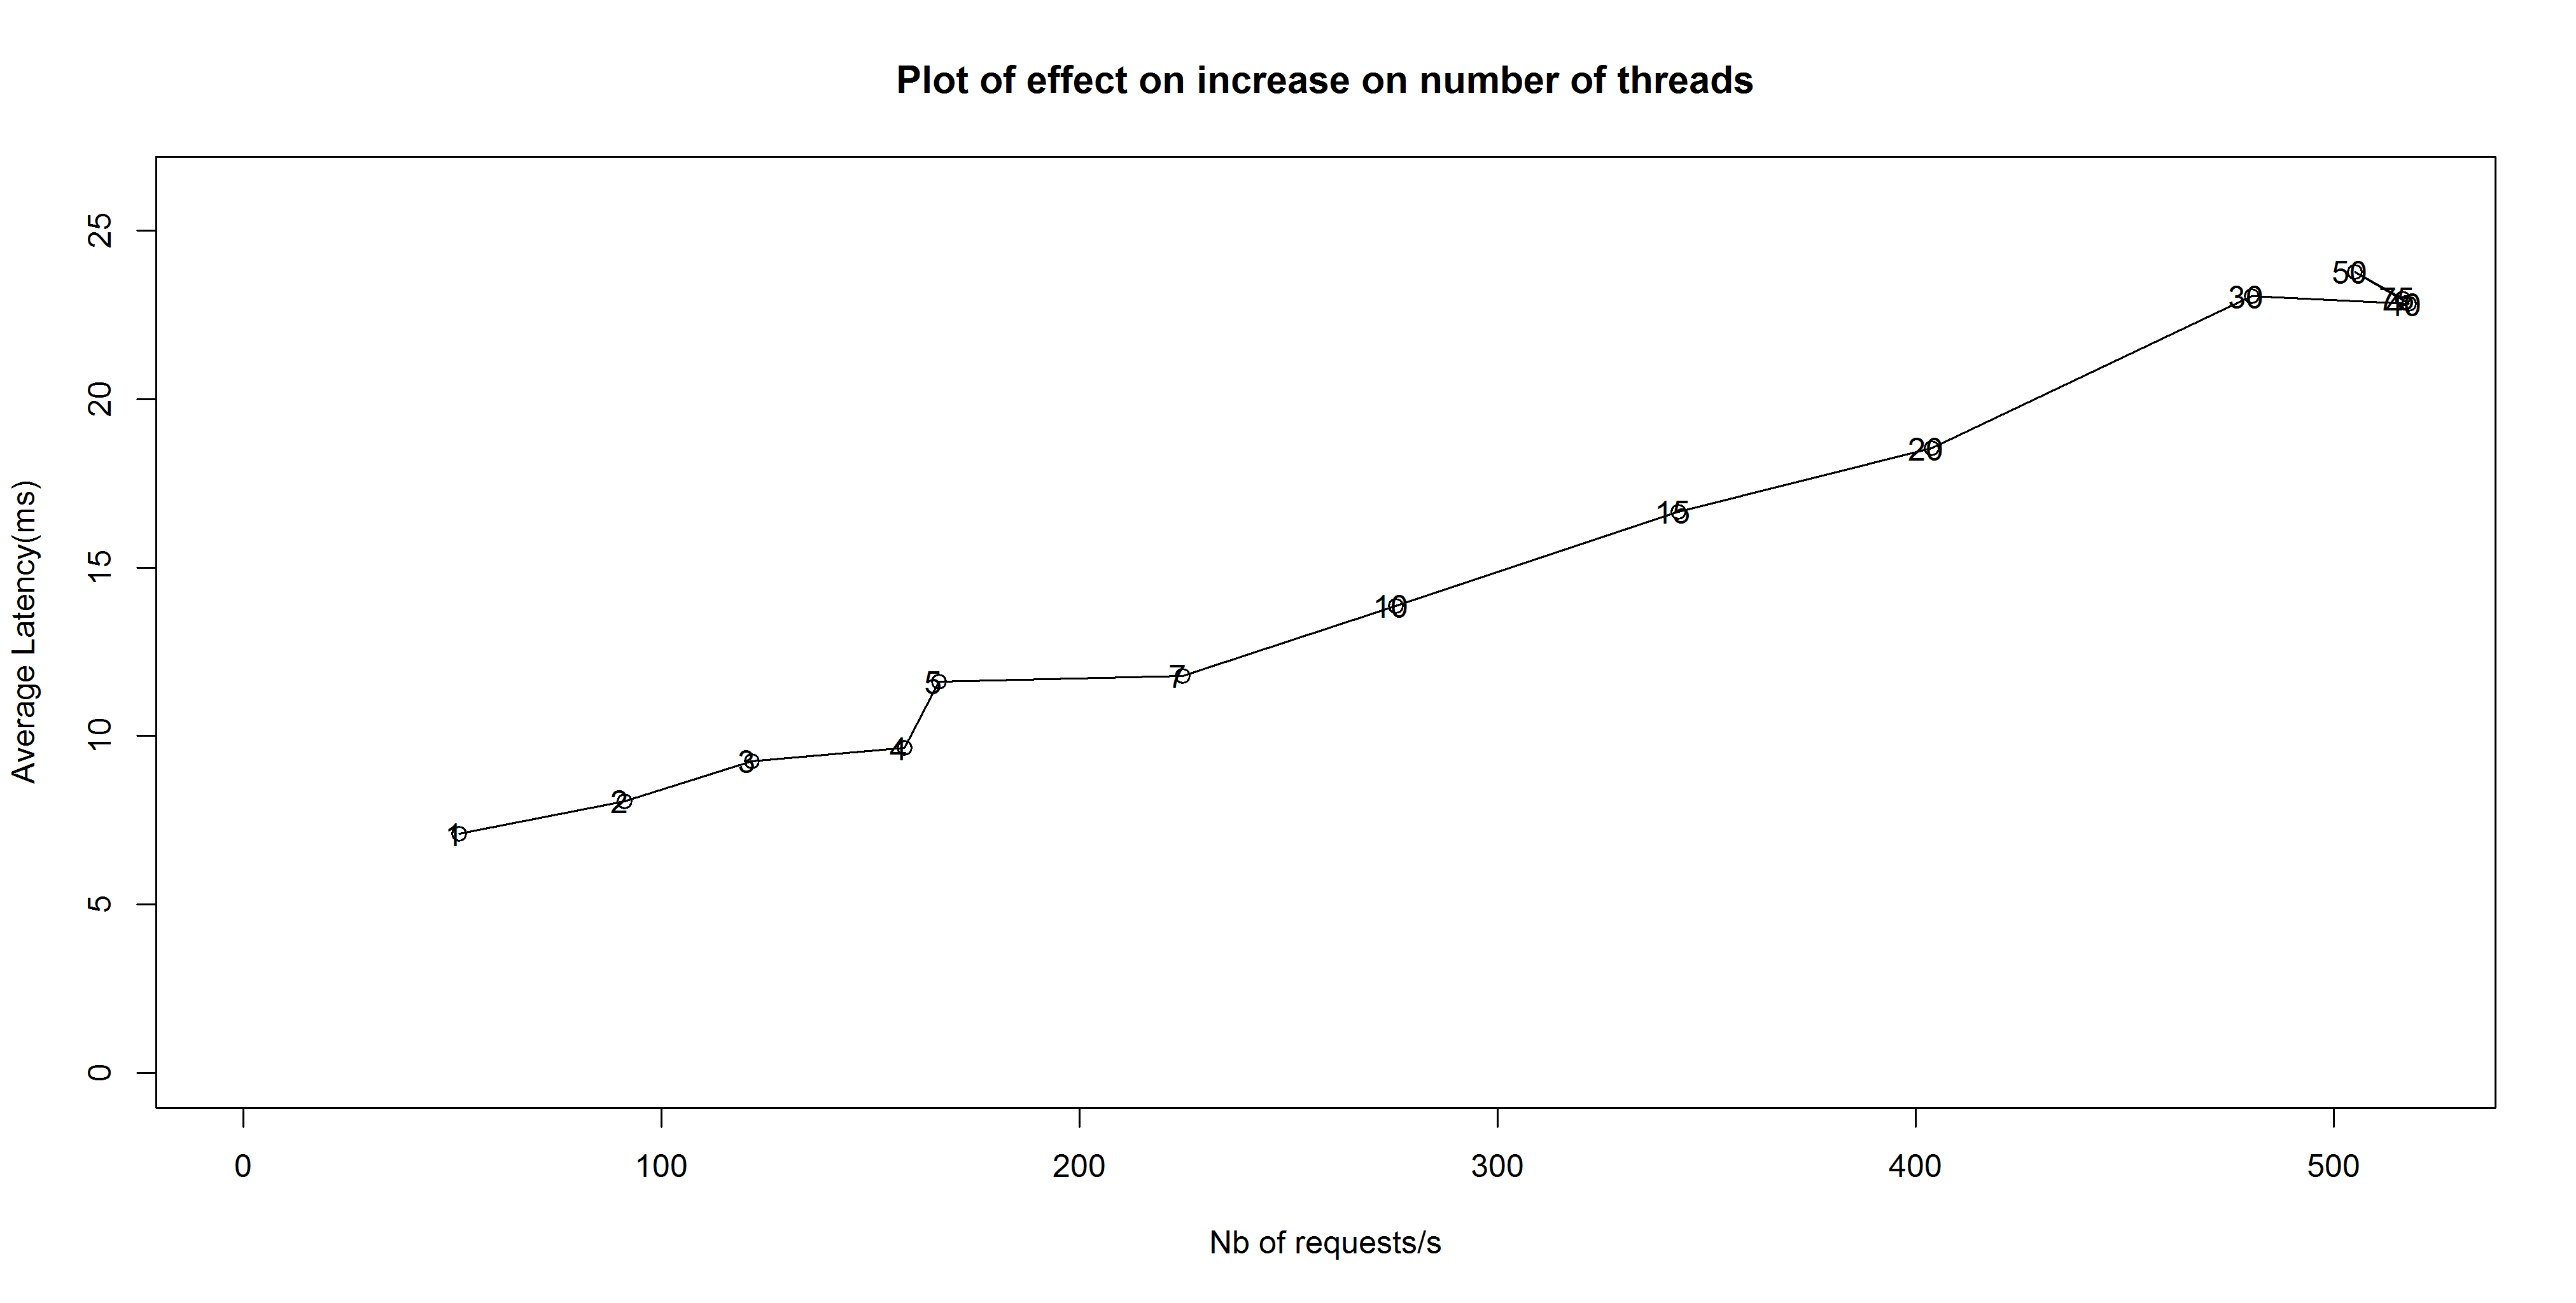
\includegraphics[width=0.41\textwidth]{img/Observaties/threads-postgresql}}
	\subfigure[HBase]{\label{fig:calibratie-gebruikers-hbase} \includegraphics[width=0.5\textwidth]{img/Observaties/threads-HBase}}
	\caption{\textbf{Kalibratie}: Overzicht van het aantal queries tot de gemiddelde vertraging voor verschillend aantal gebruikers. Elk datapunt stelt een verschillend aantal gebruikers voor met het aantal rechtsboven het punt. \newline
	Op de x-as is het gemiddeld aantal queries per second getoond over een periode van 600s, op de y-as de gemiddelde vertraging in ms. Elk datapunt toont het totaal aantal queries per seconde en de gemiddelde vertraging voor verschillend aantal gebruikers (=connecties).  }
	\label{fig:calibratie-gebruikers-resultaat}
\end{figure}

\begin{table}[ht!]
	\centering
	\begin{tabular}{l| l }
		\textbf{DBMS} & Aantal gebruikers \\
		\hline
		HBase & 50 \\
		MongoDB & 15\\
		Pgpool-II & 30\\
	\end{tabular}
	\caption{Kalibratie: Aantal gebruikers per test voor de verschillende DBMS's}
	\label{table:calibratie-gebruikers-resultaat}
\end{table}

\paragraph{Aantal queries per seconde}
De resultaten voor de kalibratietest voor het aantal queries per seconden kunnen gevonden worden in de figuren \ref{fig:calibratie-queriesperseconde-hbase}, \ref{fig:calibratie-queriesperseconde-mongodb} en \ref{fig:calibratie-queriesperseconde-pgpool-ii} voor respectievelijk HBase, MongoDB en Pgpool-II. Deze figuren tonen in de bovenste figuur de gemiddelde vertraging op een query afhankelijk van het aantal queries per seconde. Naarmate het aantal queries toeneemt stijgt de vertraging, uitgezonderd bij een laag aantal queries. De onderste figuur toont op de y-as de verhouding tussen het eigenlijk aantal uitgevoerde queries per seconde t.o.v. het gevraagde aantal queries per seconde. Een fictief voorbeeld: bij het vragen van 100 queries/sec worden er in de praktijk maar 60 uitgevoerd, dit zorgt voor een waarde van $0.6$. 

Voor elk DBMS kan met behulp van beide figuren een matige belasting gekozen worden. Een matige belasting is een belasting waarbij de tweede figuur voor elk systeem de waarde 1 zo dicht mogelijk benaderd en de vertraging nog niet te veel is gestegen t.o.v. van een lage belasting. De gekozen waarde zijn te vinden in tabel \ref{table:calibratie-queriesperseconde-resultaat}. Het benaderen van de waarde 1 bij de tweede figuur is nodig zodat het theoretisch aantal bewerkingen ook in de praktijk gehaald worden, anders is er ergens een bottleneck en is de belasting dus niet matig. De testen zouden ook uitgevoerd kunnen worden onder een andere belasting en de resultaten zouden vergeleken kunnen worden. 

\begin{figure}[htb!] 
	\centering
	\subfigure[Gemiddelde vertraging bij een verandering in aantal queries per seconde.] {\label{fig:calibratie-queriesperseconde-hbase-1} 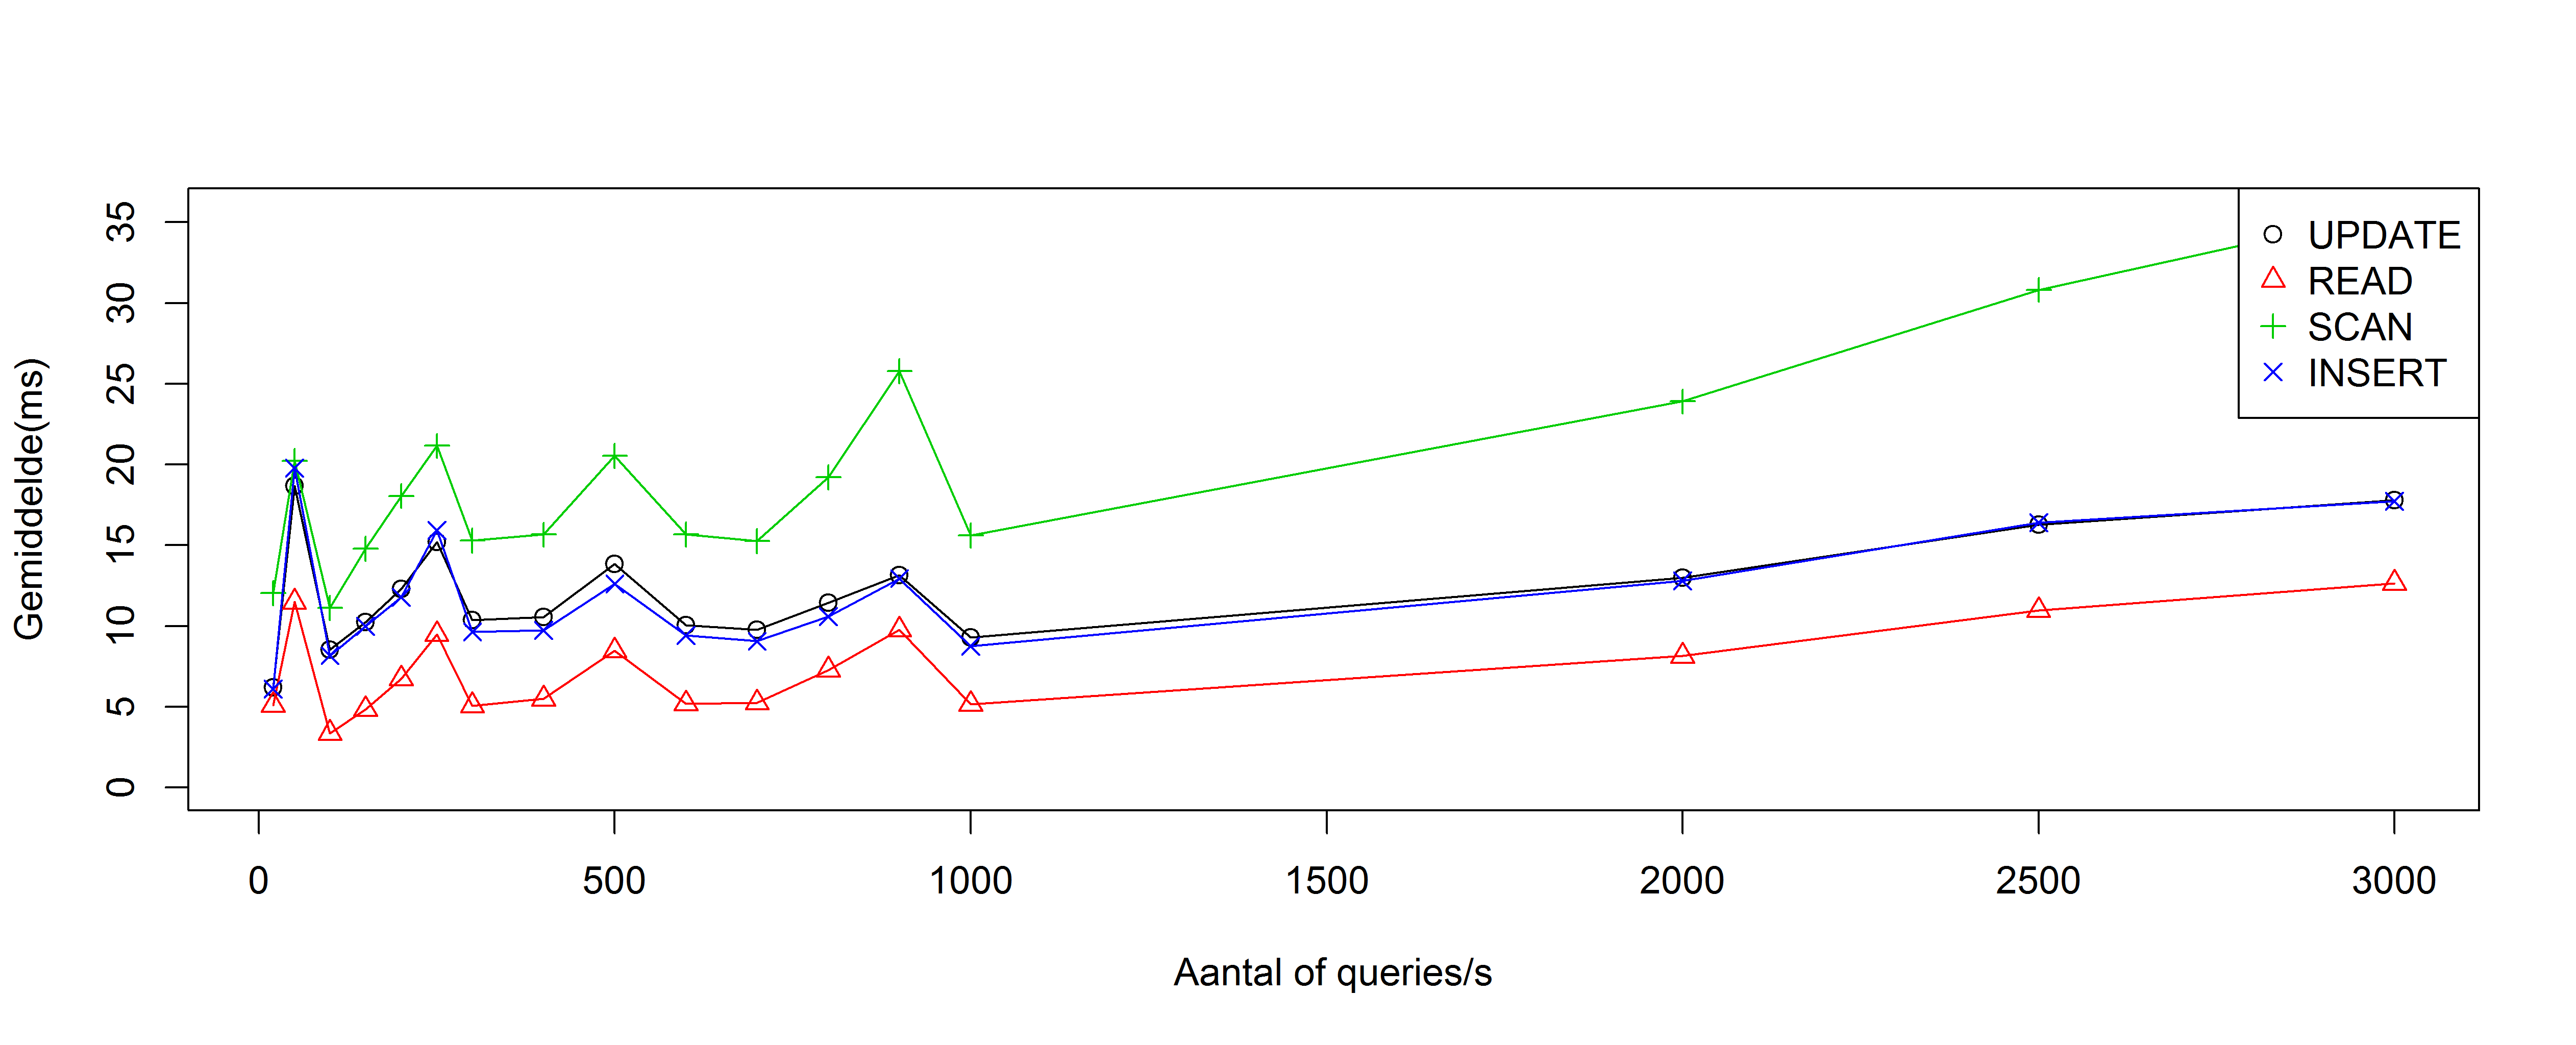
\includegraphics[width=0.95\textwidth]{img/Observaties/loadbalance-db-HBase}}
	\subfigure[Verhouding van het aantal uitgevoerde queries ten opzichte van het aantal gevraagde queries.] {\label{fig:calibratie-queriesperseconde-hbase-2} 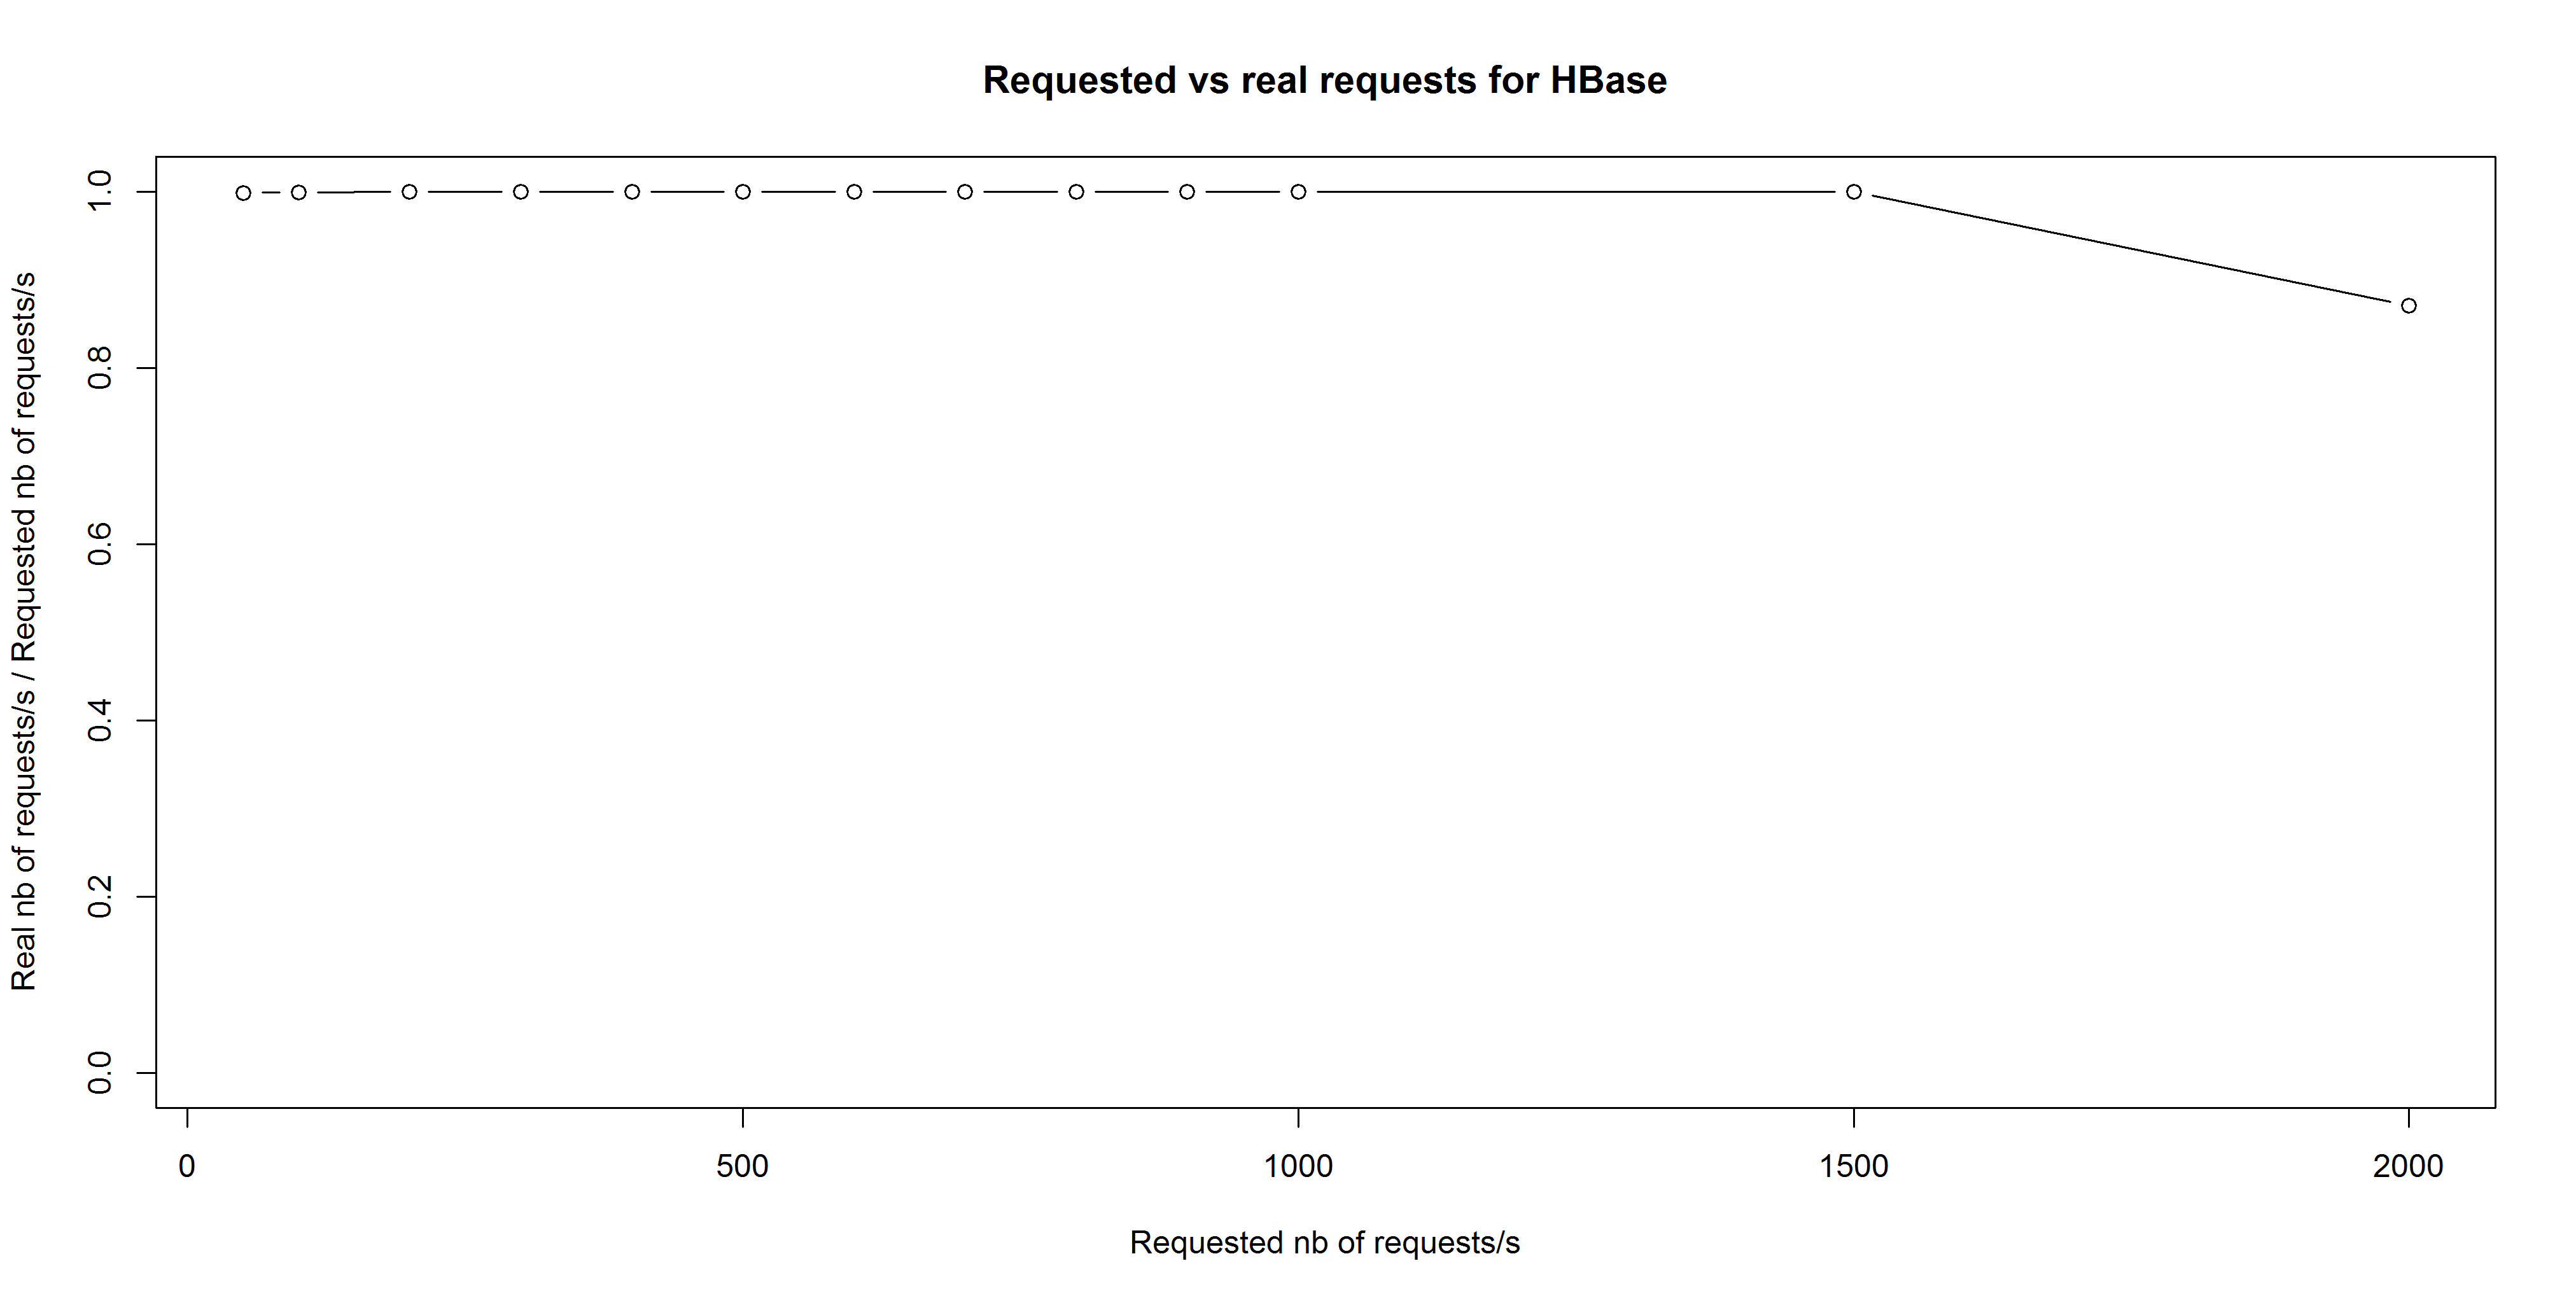
\includegraphics[width=0.95\textwidth]{img/Observaties/loadbalance-realthroughput-db-HBase}}
	\caption{Kalibratie: Overzicht van de vertraging t.o.v. het theoretisch aantal aanvragen met een vergelijking hoeveel werkelijke aanvragen er waren voor HBase. }
	\label{fig:calibratie-queriesperseconde-hbase}
\end{figure}

\begin{figure}[htb!] 
	\centering
	\subfigure[Gemiddelde vertraging bij een verandering in aantal queries per seconde.] {\label{fig:calibratie-queriesperseconde-mongodb-1} 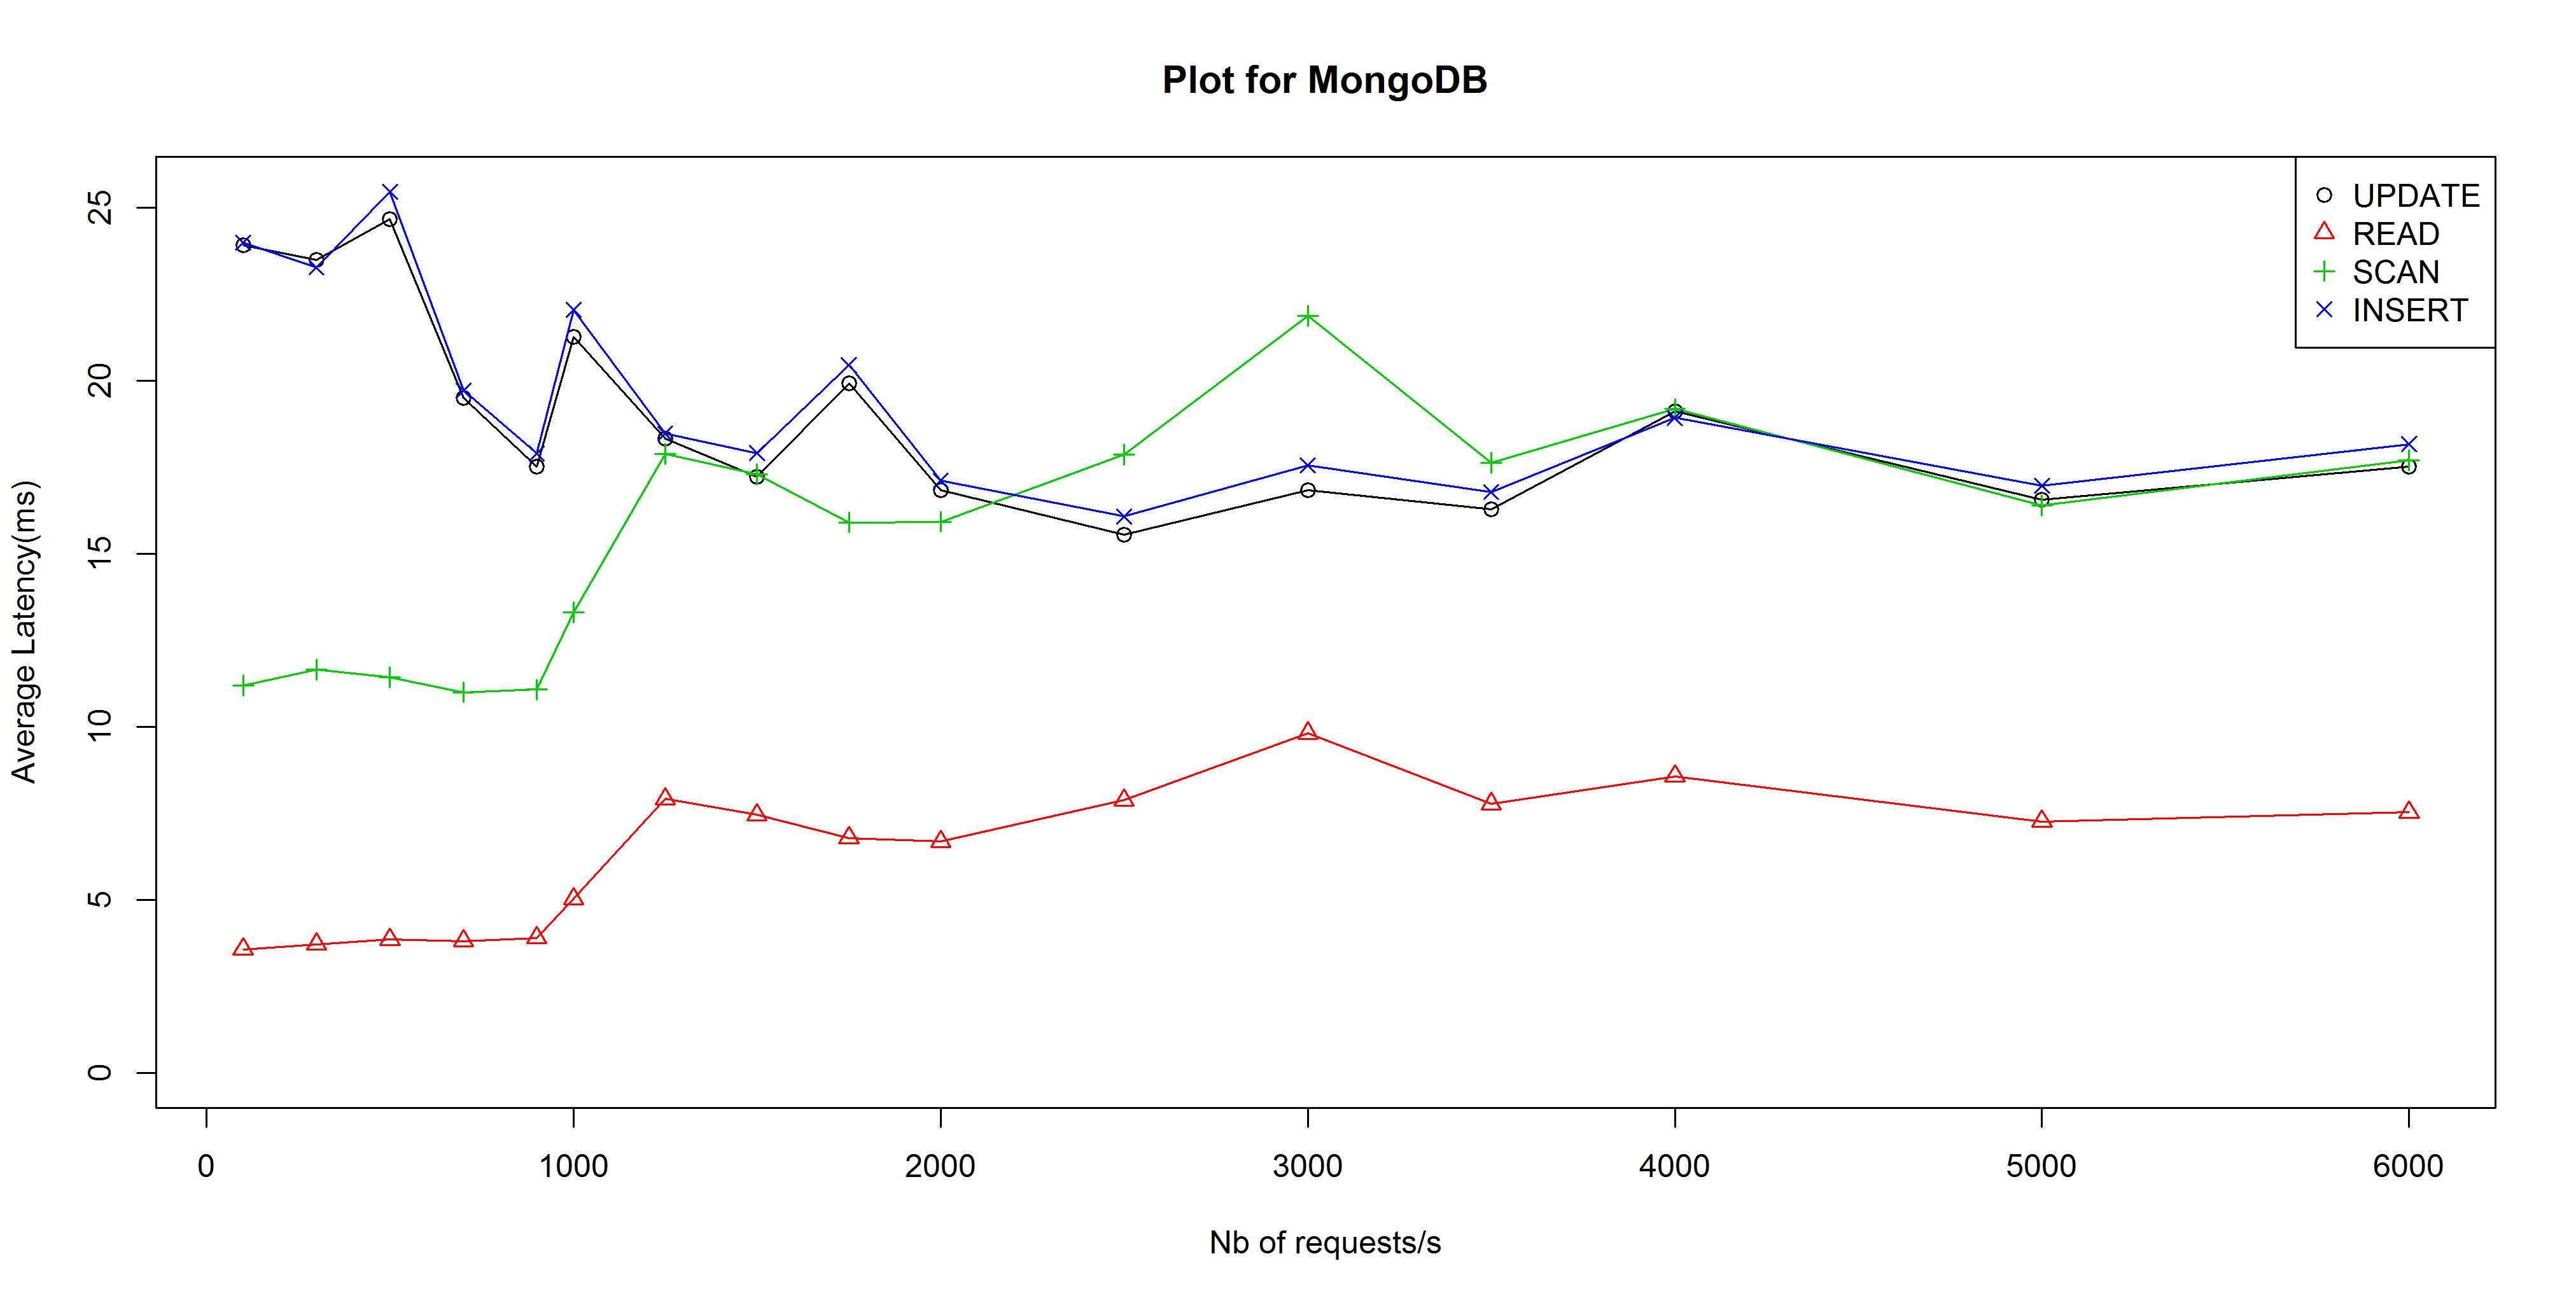
\includegraphics[width=0.95\textwidth]{img/Observaties/loadbalance-db-MongoDB}}
	\subfigure[Verhouding van het aantal uitgevoerde queries ten opzichte van het aantal gevraagde queries.] {\label{fig:calibratie-queriesperseconde-mongodb-2} 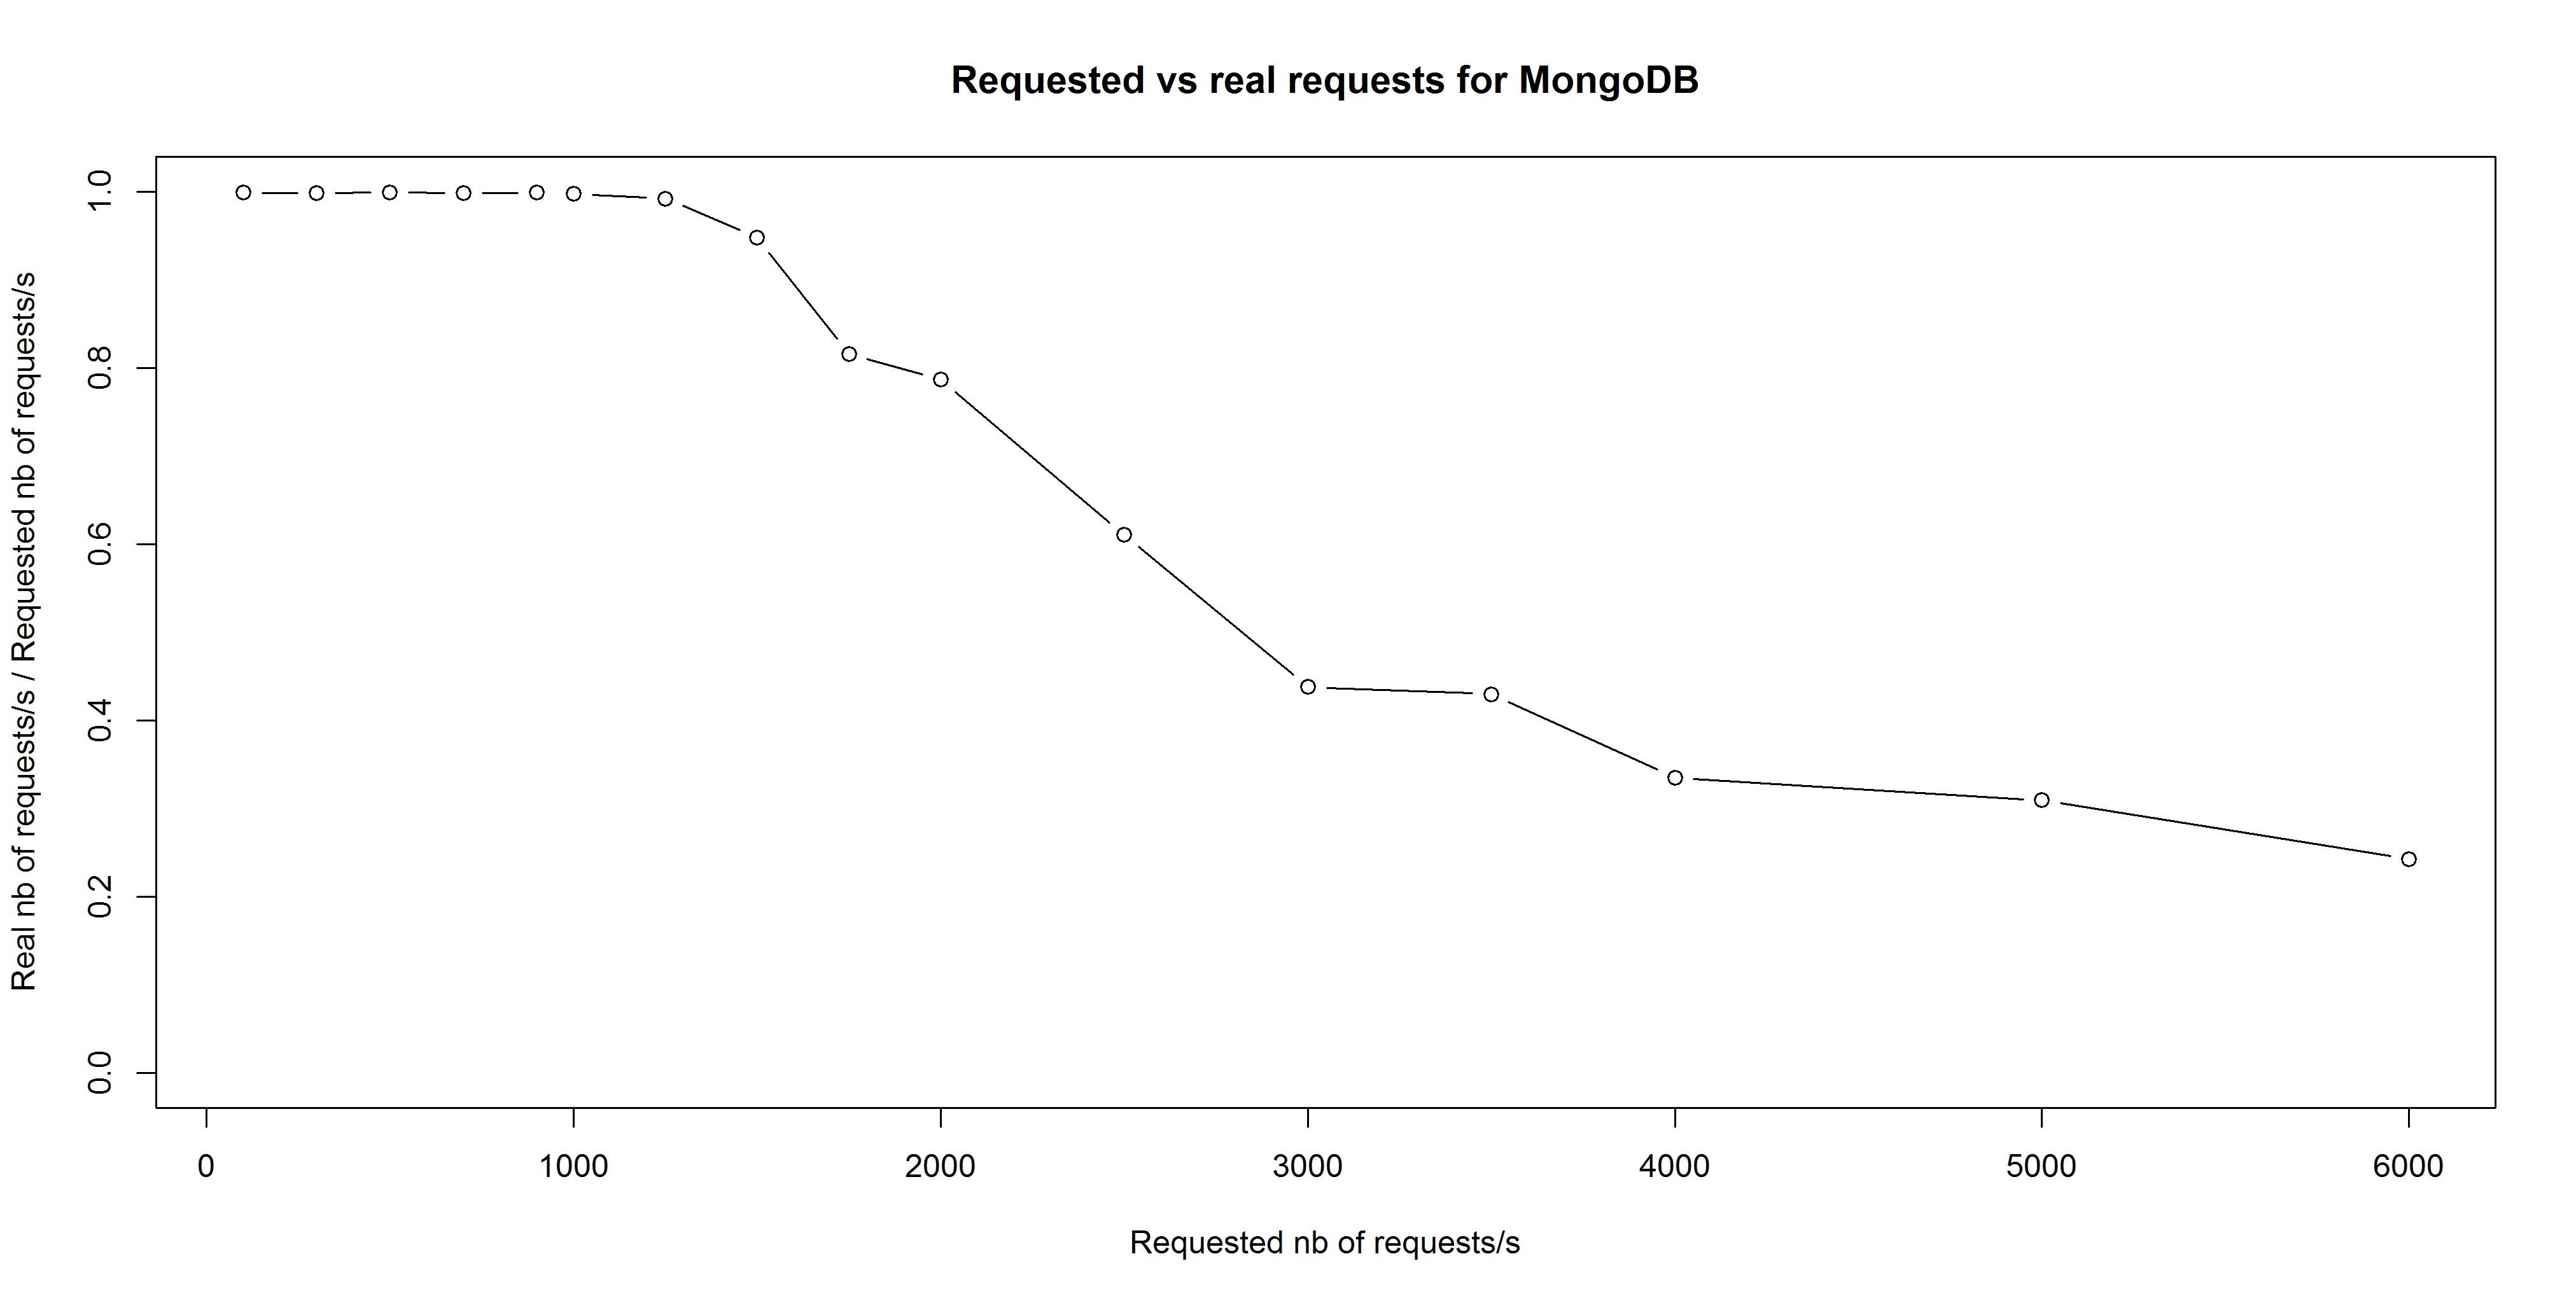
\includegraphics[width=0.95\textwidth]{img/Observaties/loadbalance-realthroughput-db-MongoDB}}
	\caption{Kalibratie: Overzicht van de vertraging t.o.v. het theoretisch aantal aanvragen met een vergelijking hoeveel werkelijke aanvragen er waren voor MongoDB. }
	\label{fig:calibratie-queriesperseconde-mongodb}
\end{figure}

\begin{figure}[htb!] 
	\centering
	\subfigure[Gemiddelde vertraging bij een verandering in aantal queries per seconde.] {\label{fig:calibratie-queriesperseconde-pgpool-ii-1} 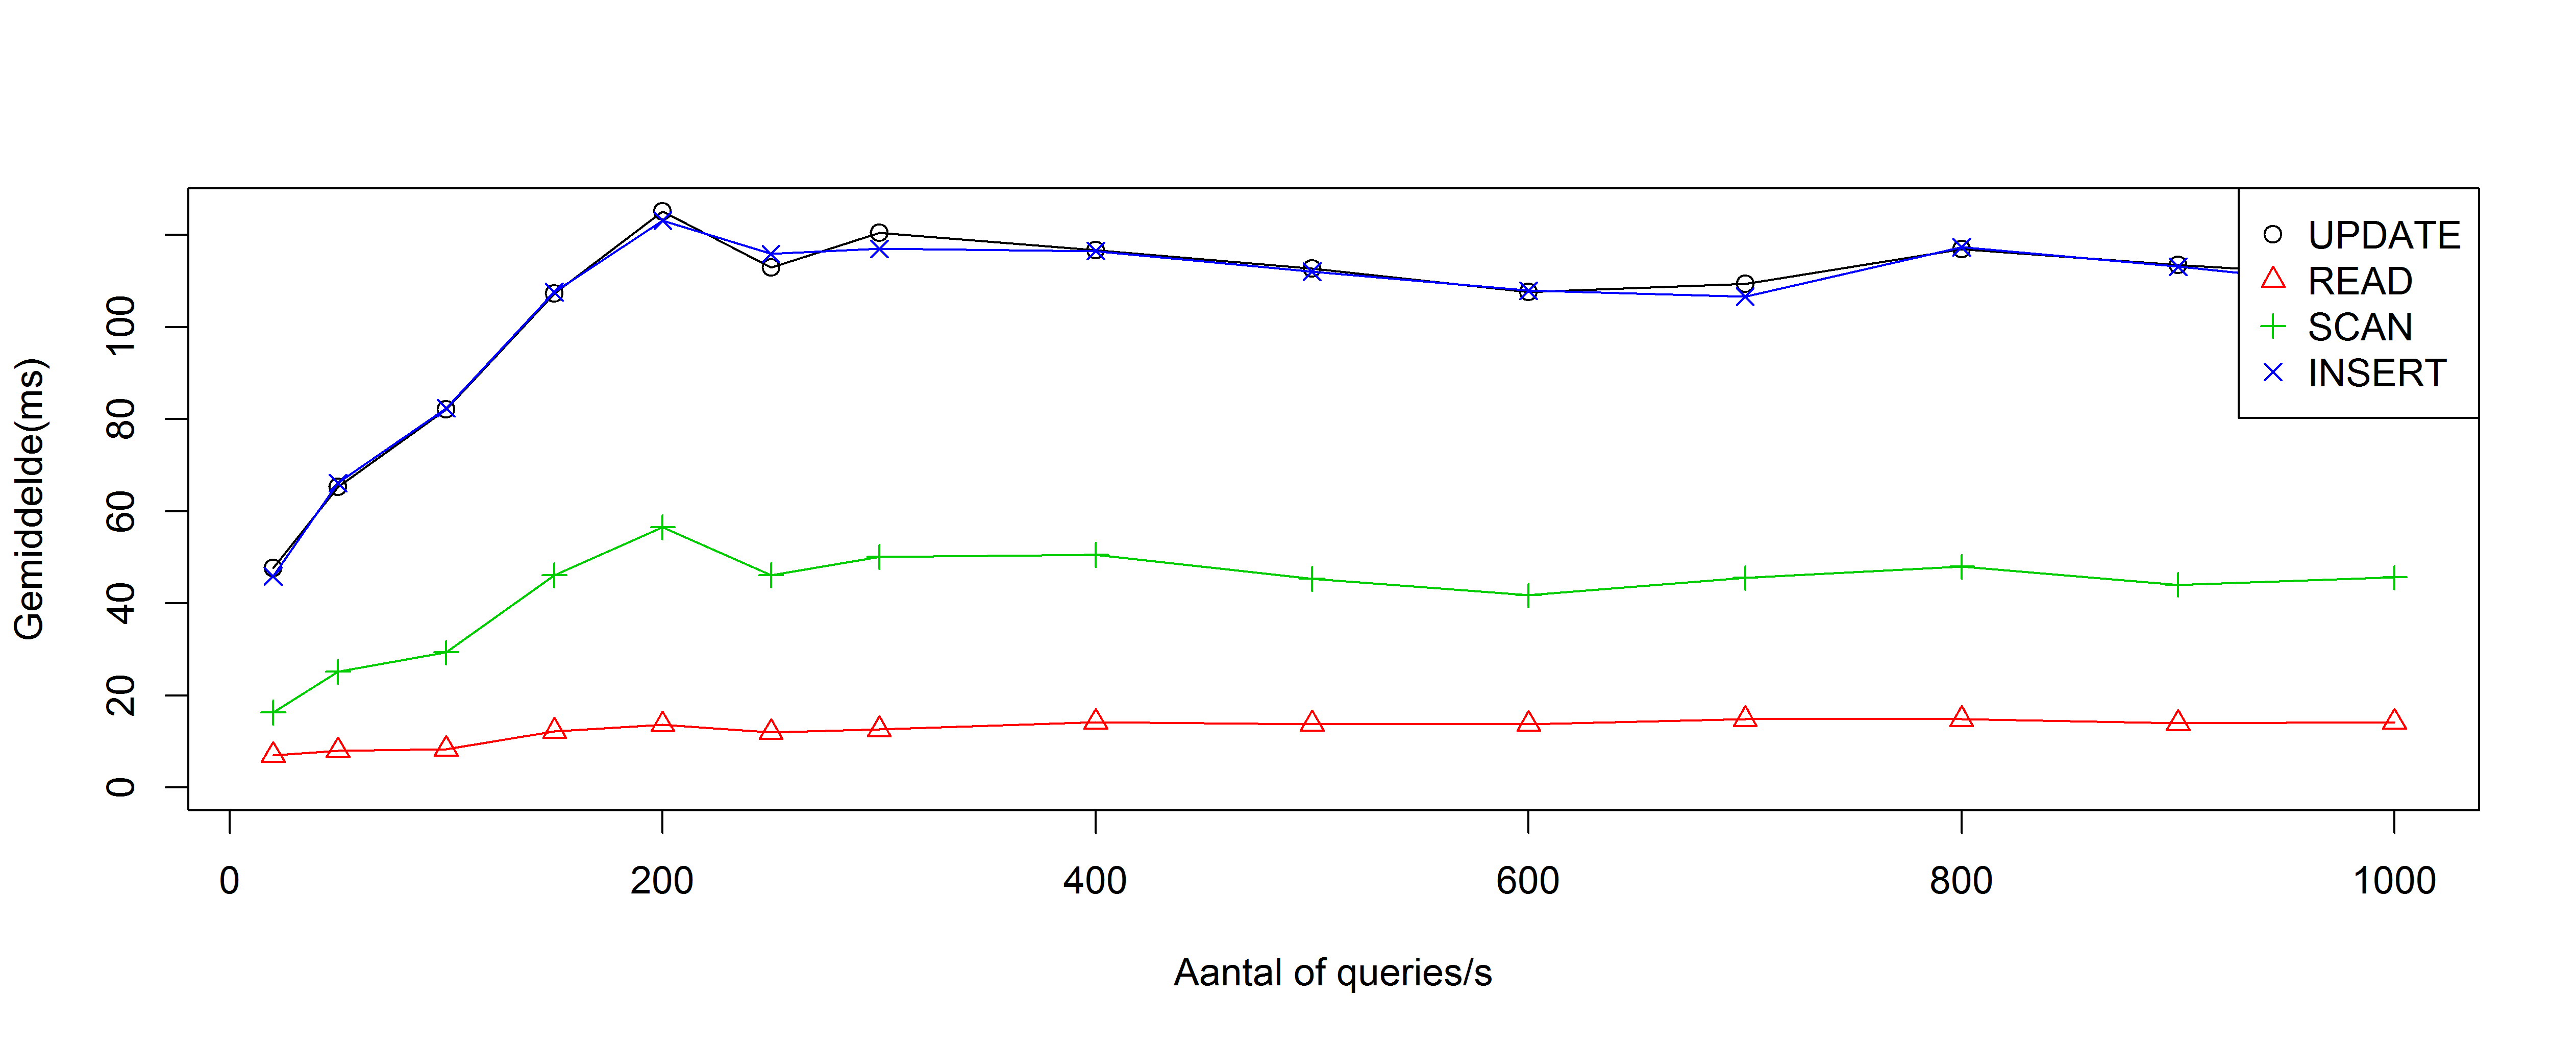
\includegraphics[width=0.95\textwidth]{img/Observaties/loadbalance-db-PostgreSQL}}
	\subfigure[Verhouding van het aantal uitgevoerde queries ten opzichte van het aantal gevraagde queries.] {\label{fig:calibratie-queriesperseconde-pgpool-ii-2} 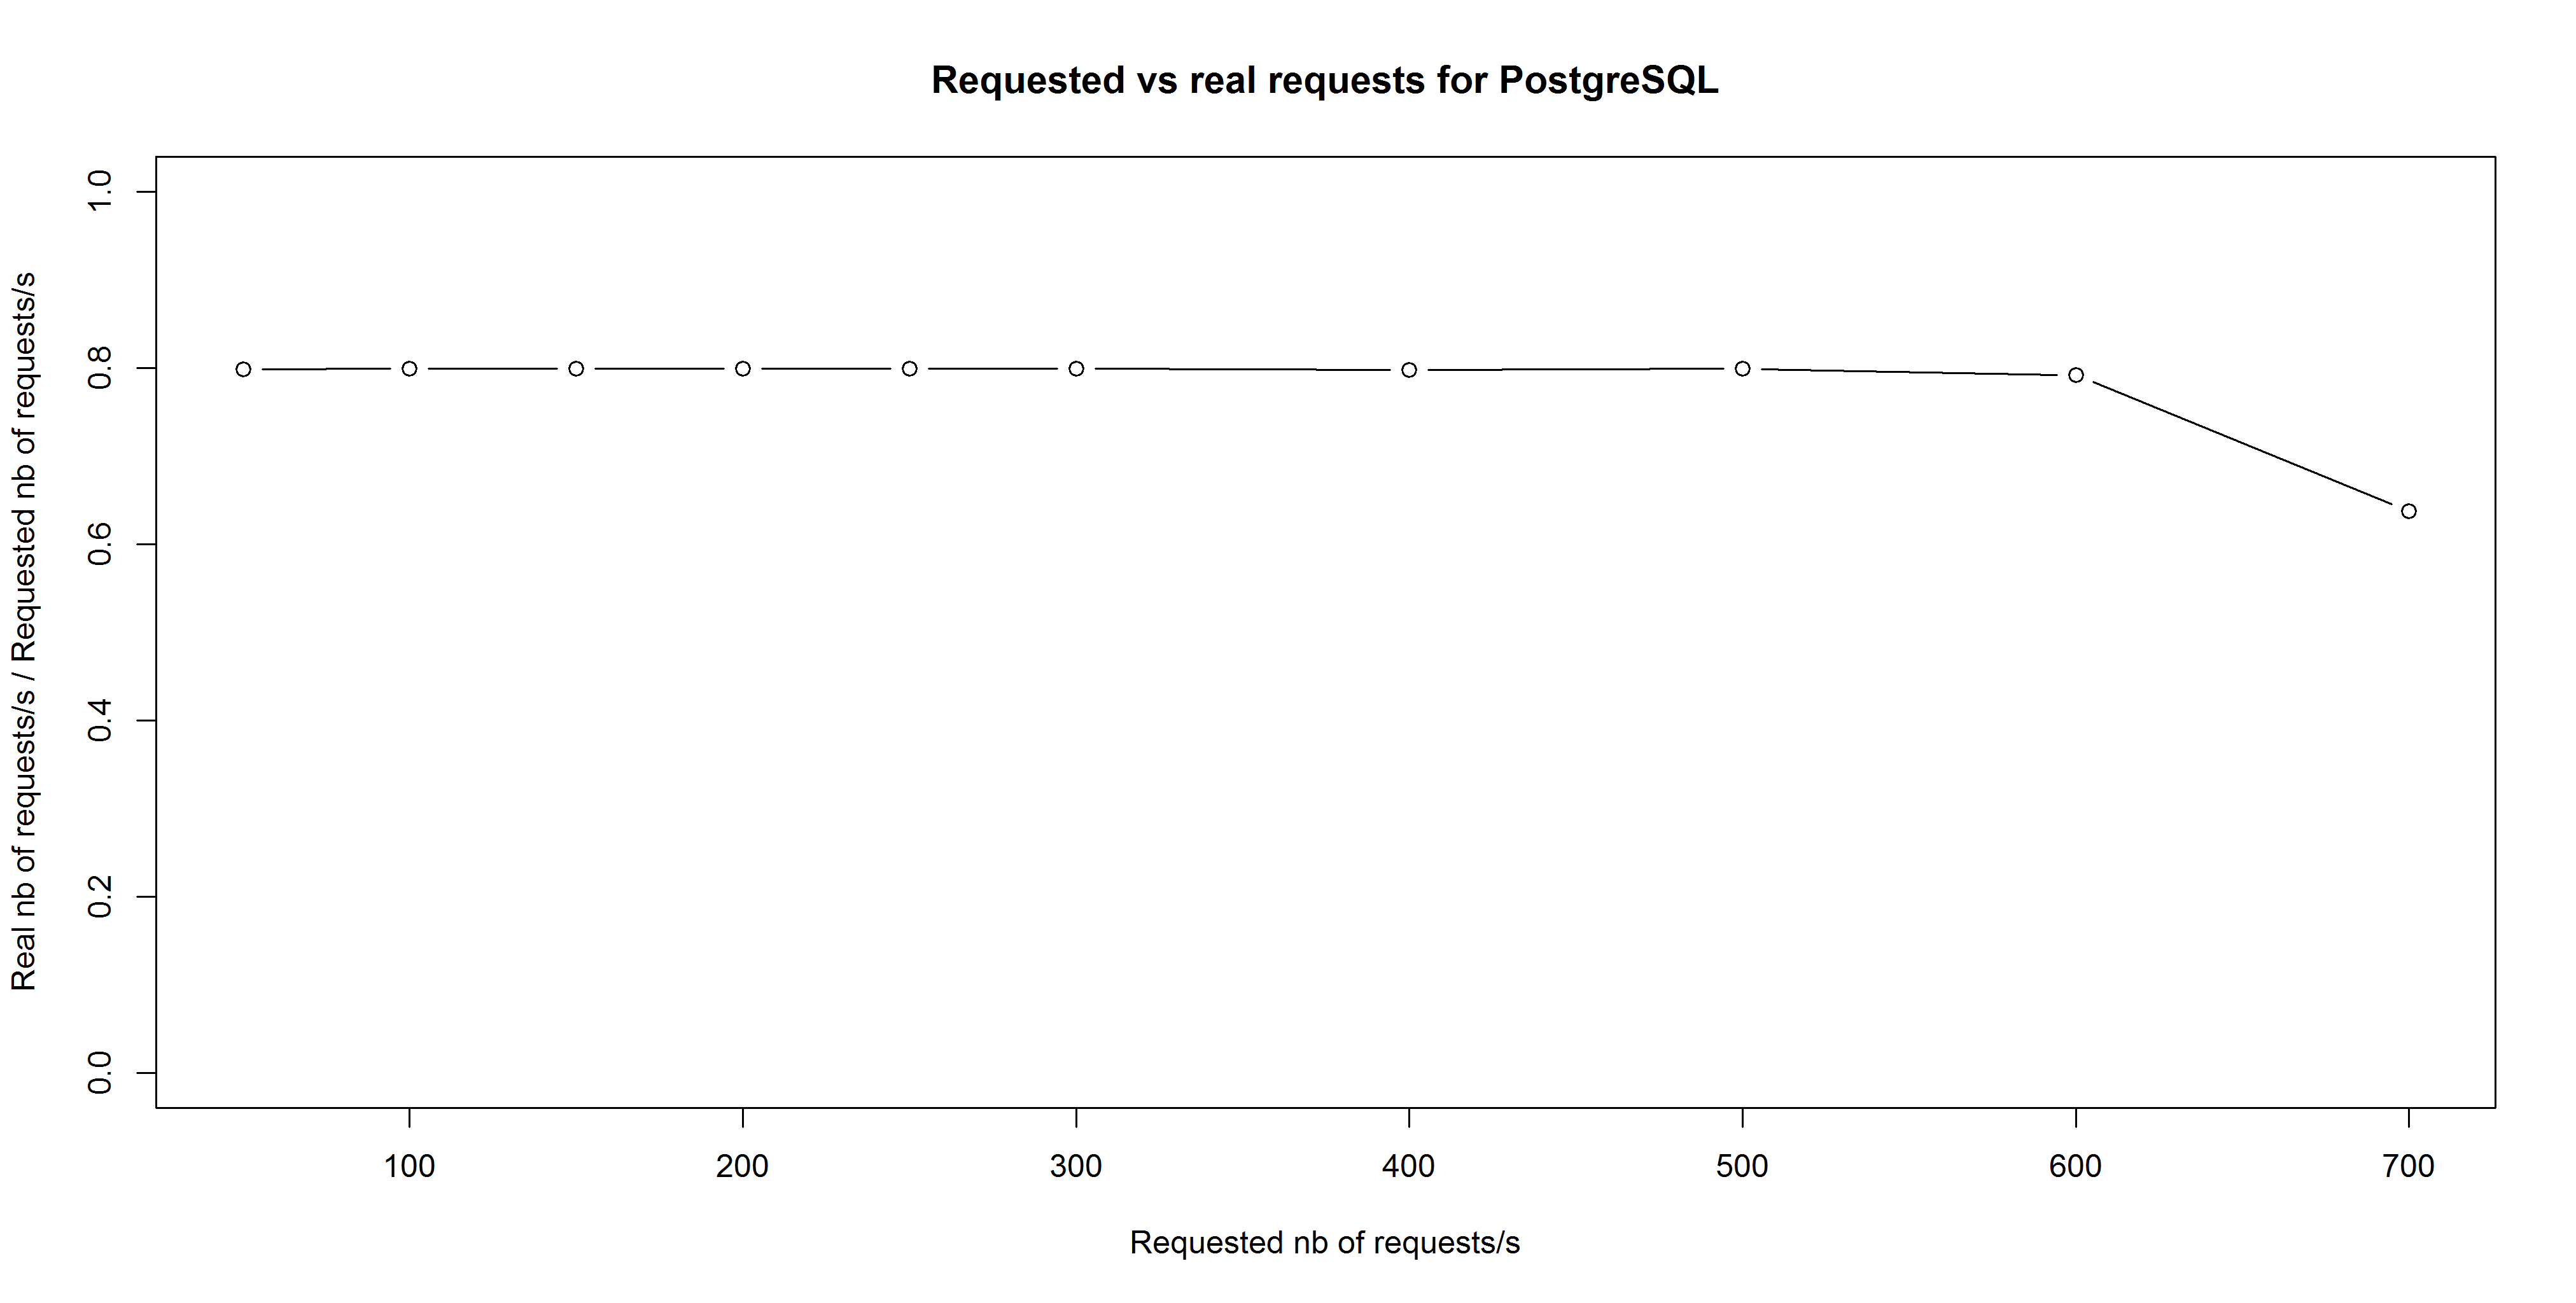
\includegraphics[width=0.95\textwidth]{img/Observaties/loadbalance-realthroughput-db-PostgreSQL}}
	\caption{Kalibratie: Overzicht van de vertraging t.o.v. het theoretisch aantal aanvragen met een vergelijking hoeveel werkelijke aanvragen er waren voor Pgpool-II. }
	\label{fig:calibratie-queriesperseconde-pgpool-ii}
\end{figure}

\begin{table}[htb!]
	\centering
	\begin{tabular}{l| l }
		\textbf{DBMS} & Aantal requests per seconde \\
		\hline
		HBase & 600 \\
		MongoDB & 200\\
		Pgpool-II & 100\\
	\end{tabular}
	\caption{Kalibratie: Aantal queries per seconde per test bij een matige belasting voor de verschillende DBMS's.}
	\label{table:calibratie-queriesperseconde-resultaat}
\end{table}


\FloatBarrier 
\section{Beschikbaarheidstest}
Bij de beschikbaarheidstesten kunnen de gegevens op verschillende manieren voorgesteld worden: de vertraging per query over de hele test, de vertraging tijdens het stoppen en starten van systemen of een vergelijking van de vertraging voor het stoppen (150-250s), tussen het stoppen en starten(400-500s) en na het herstarten (700-800s). 

Voor elk systeem zullen enkele grafieken getoond worden, de rest zal besproken worden in de tekst bij de figuren. De grafieken van al de testen zijn beschikbaar via de link gegeven in het begin van het hoofdstuk. 

Een punt op de grafiek stelt de gemiddelde vertraging van 1 seconde voor, de lijn het gemiddelde over 10 seconden. 


\begin{figure}[ht!] 
	\centering
	\subfigure{\label{fig:beschikbaar-hbase-soft} 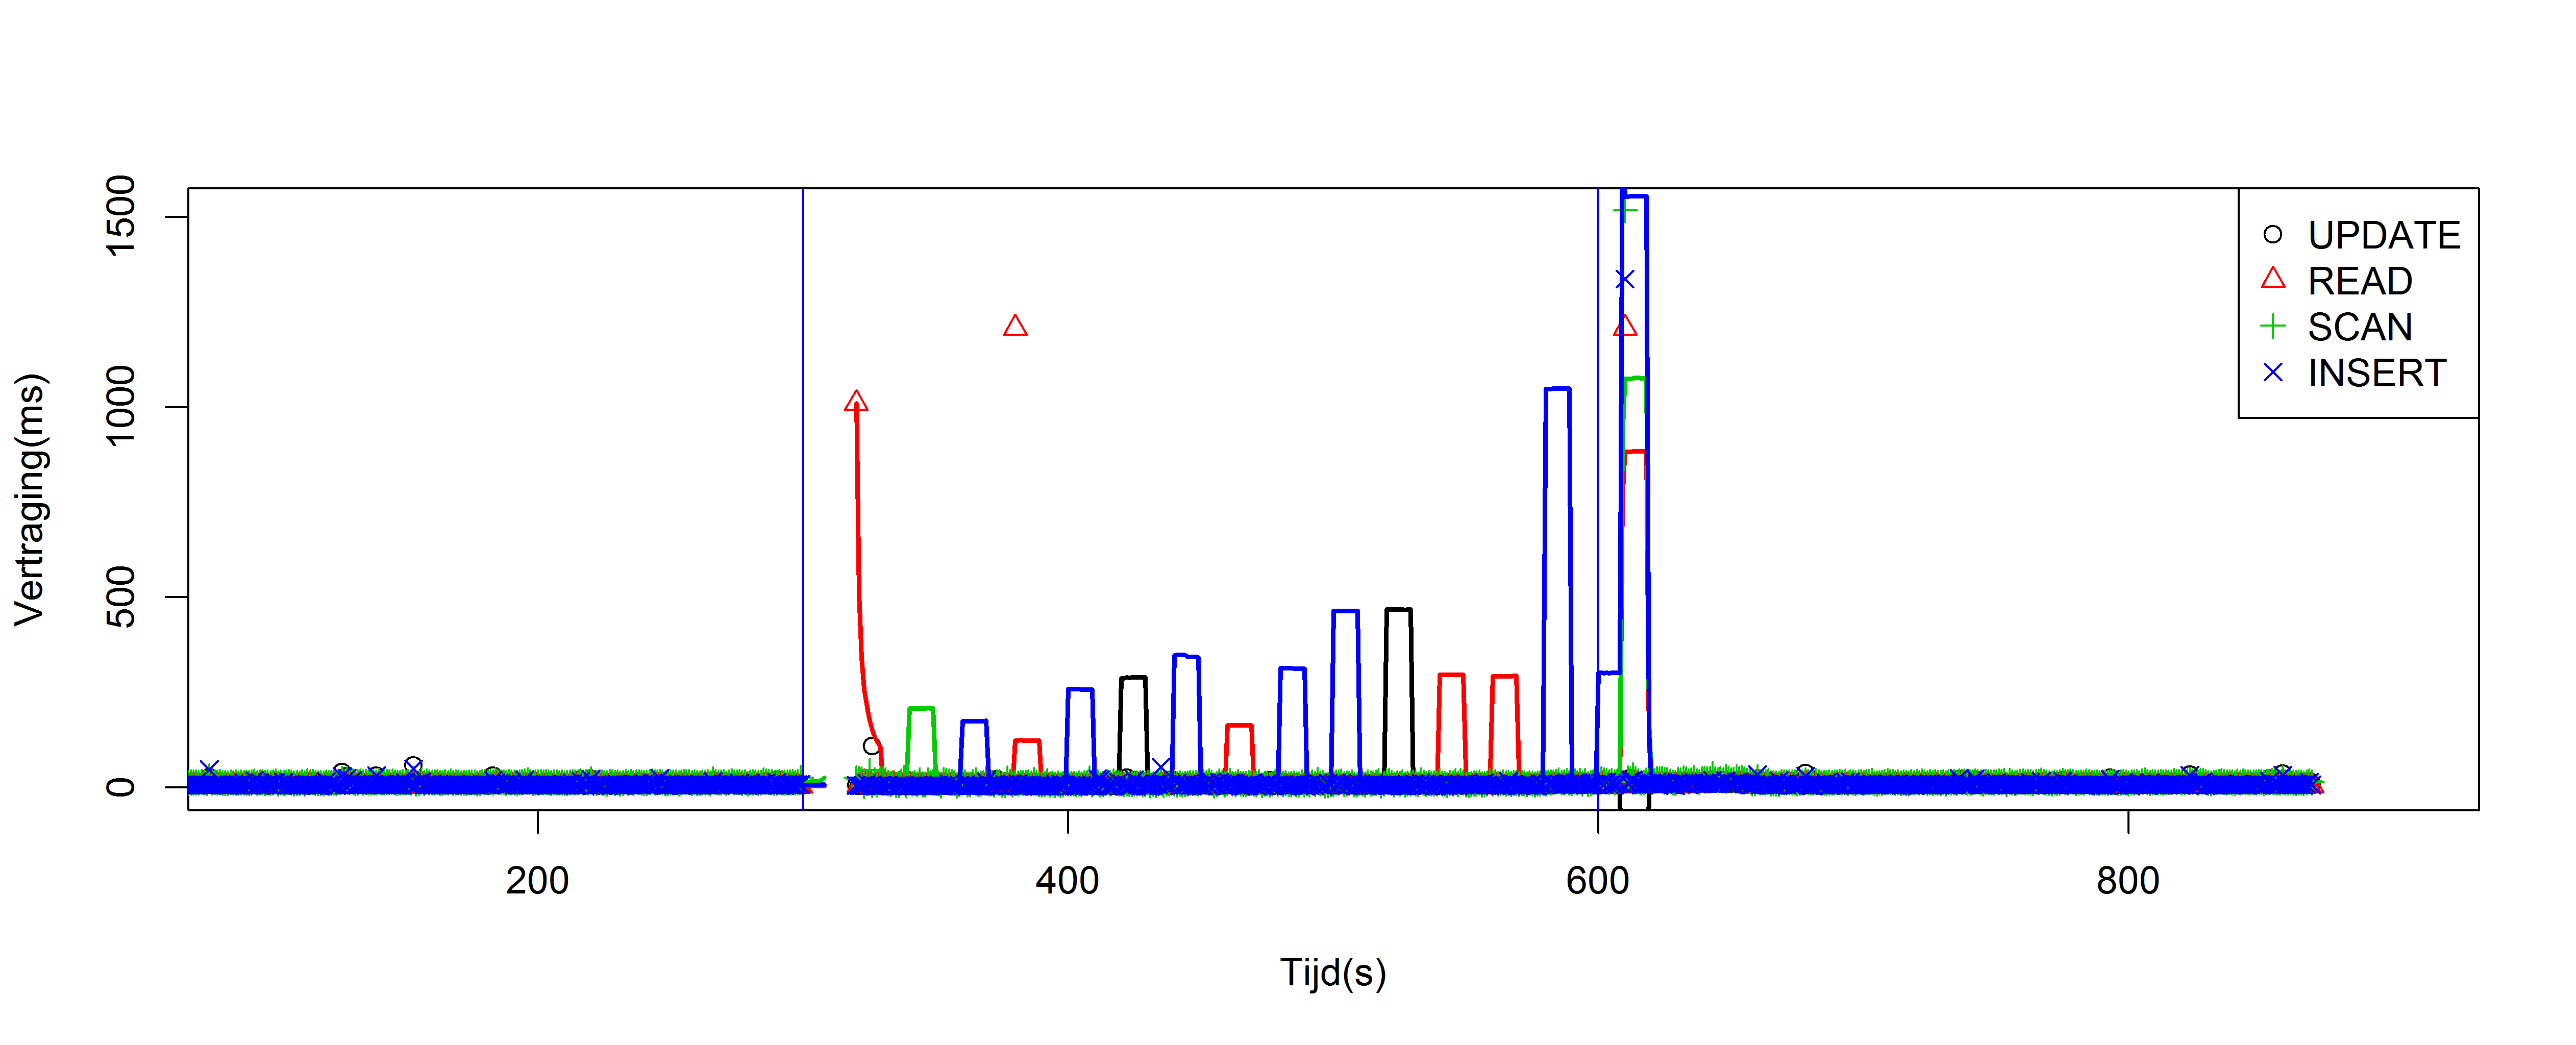
\includegraphics[width=0.9\textwidth]{img/Observaties/HBase/single-graph-2-1}}
	\subfigure{\label{fig:beschikbaar-hbase-drop} 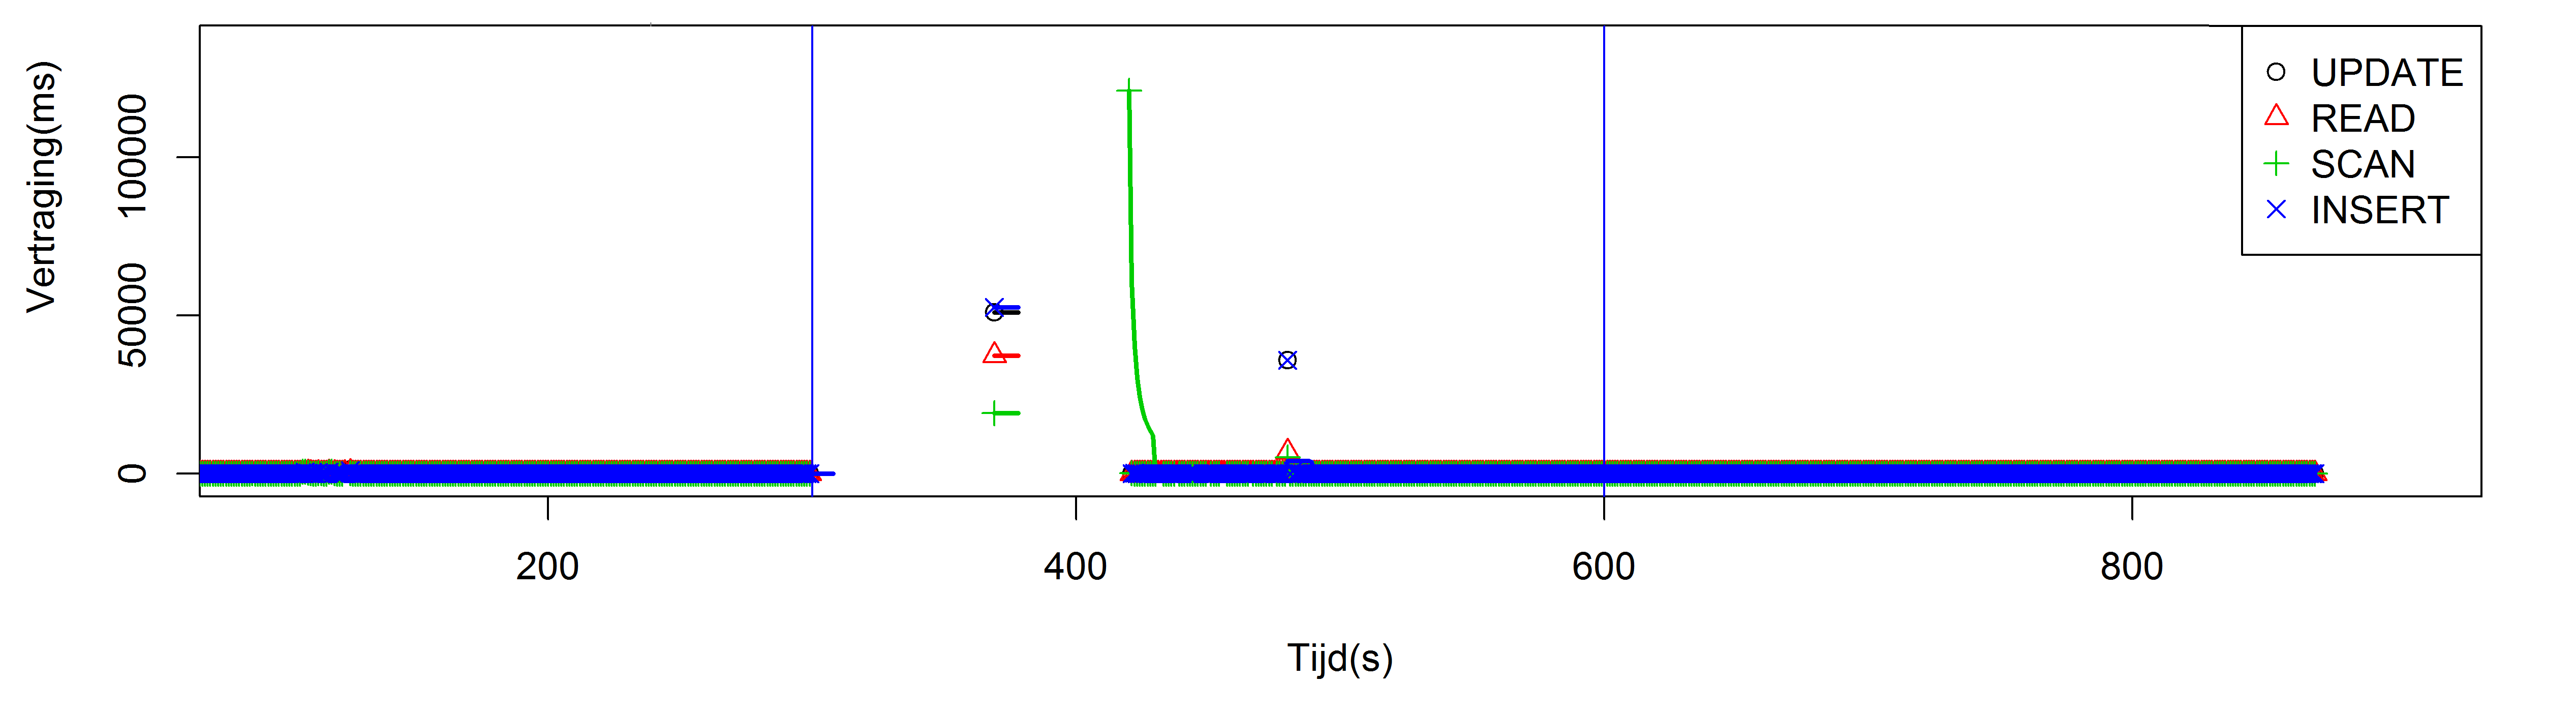
\includegraphics[width=0.9\textwidth]{img/Observaties/HBase/single-graph-2-drop-1}}
	\subfigure{\label{fig:beschikbaar-hbase-hard} 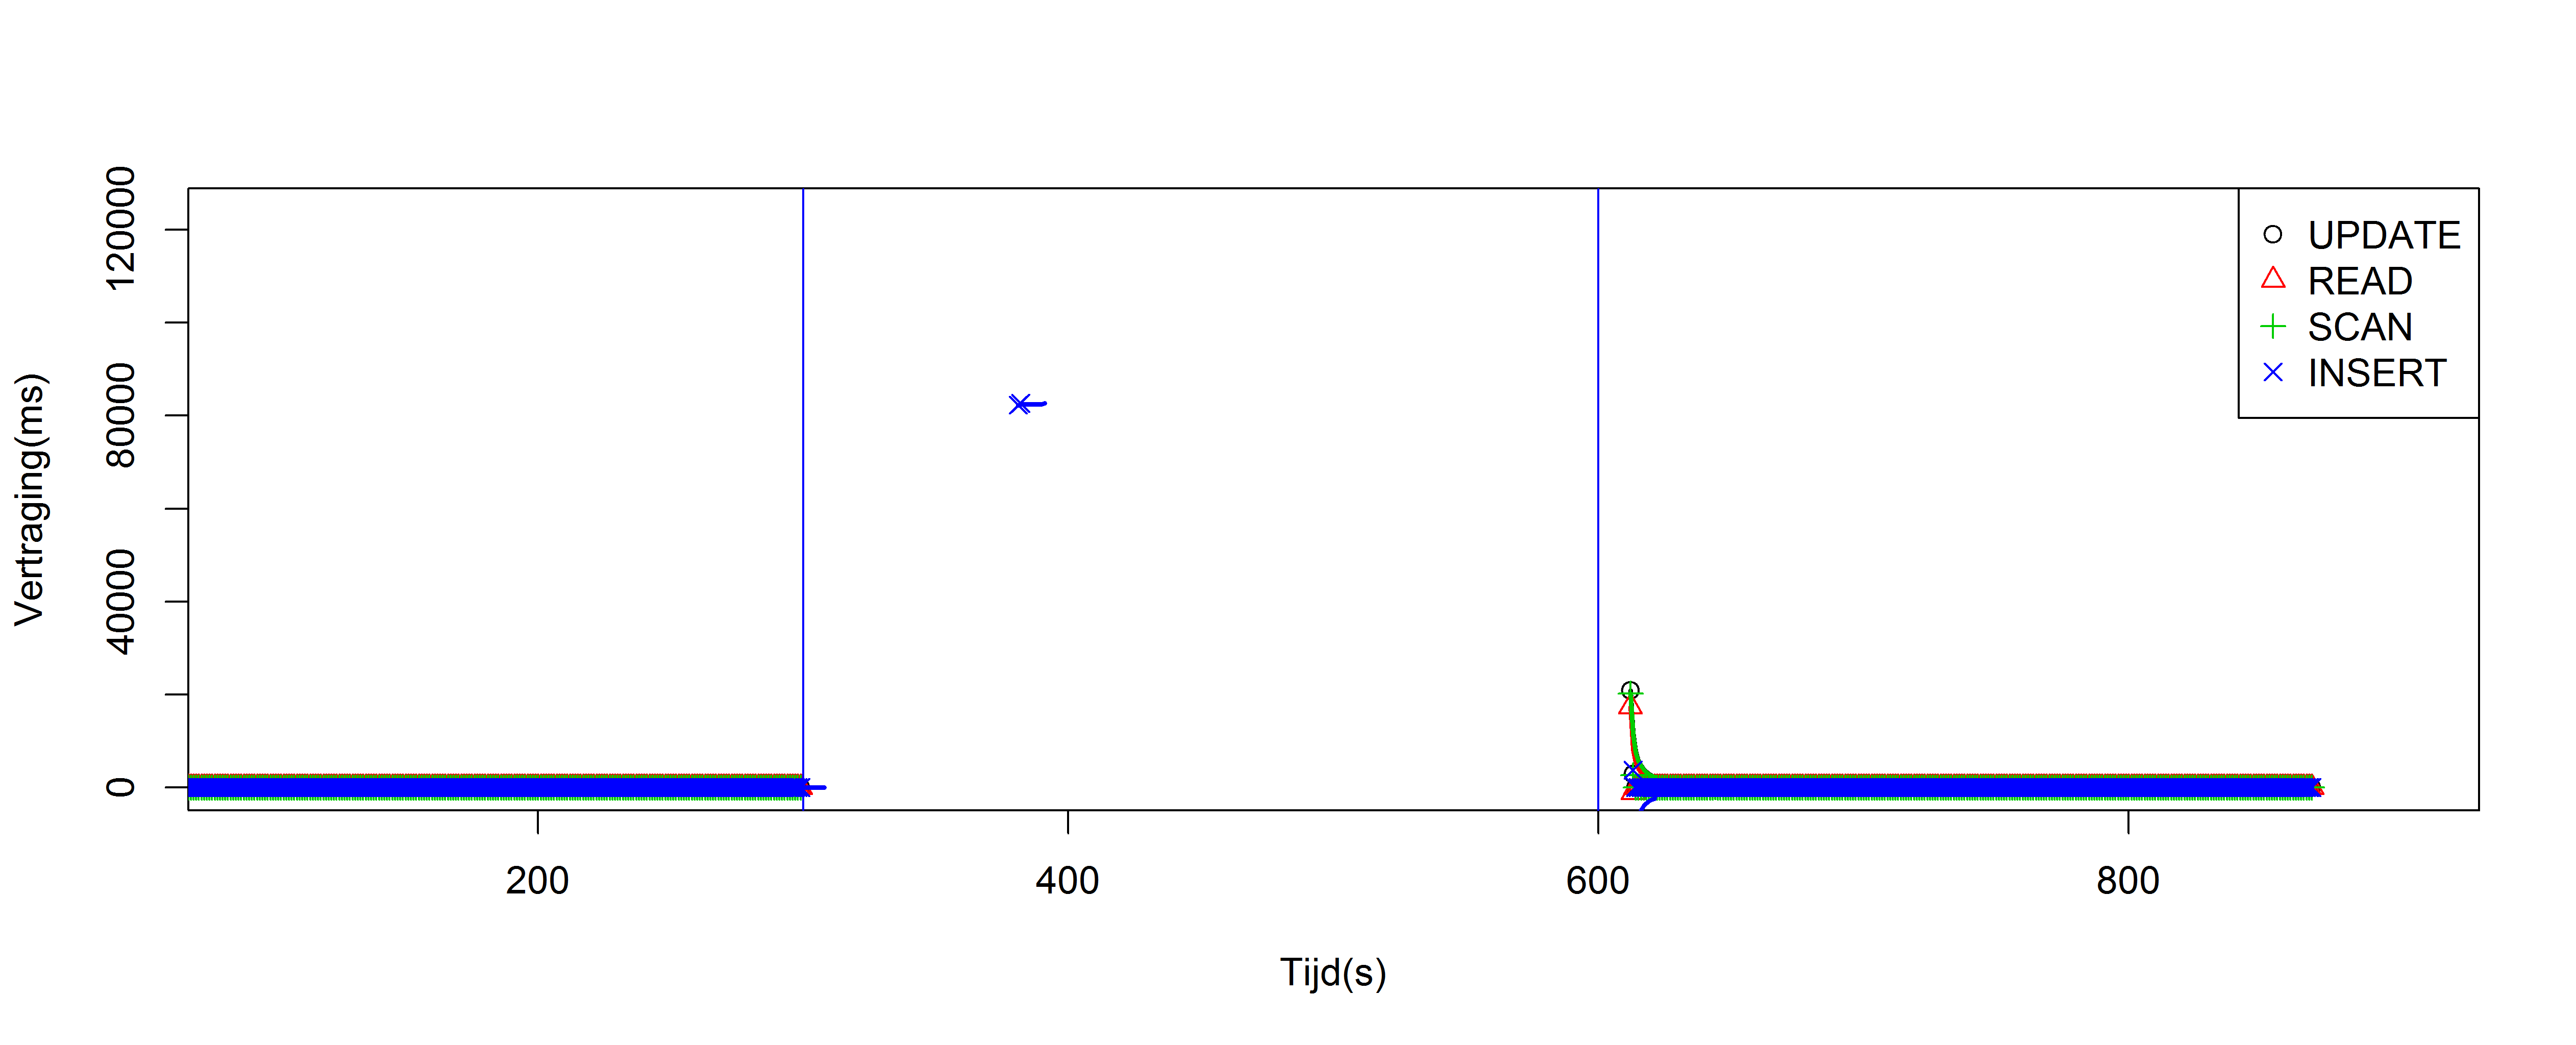
\includegraphics[width=0.9\textwidth]{img/Observaties/HBase/single-graph-3-kill-1}}
	\caption{\textbf{Beschikbaarheid van HBase} \newline 
	Bij HBase zijn er verschillende reacties op het stopzetten van een node. Zo kun je in de eerste figuur een zachte stop zien. Bij het zacht stoppen van een instantie, is er een onderbreking van ongeveer 20 seconde. Daarna kunnen er af en toe nog verhogingen in de queries optreden. \newline
	De tweede figuur stelt een netwerkonderbreking voor, er is een onderbreking van gemiddeld ongeveer 100 seconden. Daarna is het terug stabiel. \newline
	Bij een harde stop is er een combinatie van de netwerk onderbreking én is het af en toe zo dat de volledige periode geen queries mogelijk zijn. De laatste figuur toont het resultaten wanneer er geen queries mogelijk zijn. 	 \newline
	Tijdens de onderbreking (400-500s), is er geen significante verandering in de vertraging van de uitgevoerde queries gemeten (t.o.v. 150s - 250s en 700s - 800s). 
	}
	\label{fig:beschikbaar-hbase-1}
\end{figure}

 
\begin{figure}[ht!] 
	\centering
	\subfigure{\label{fig:beschikbaar-mongodb-soft} 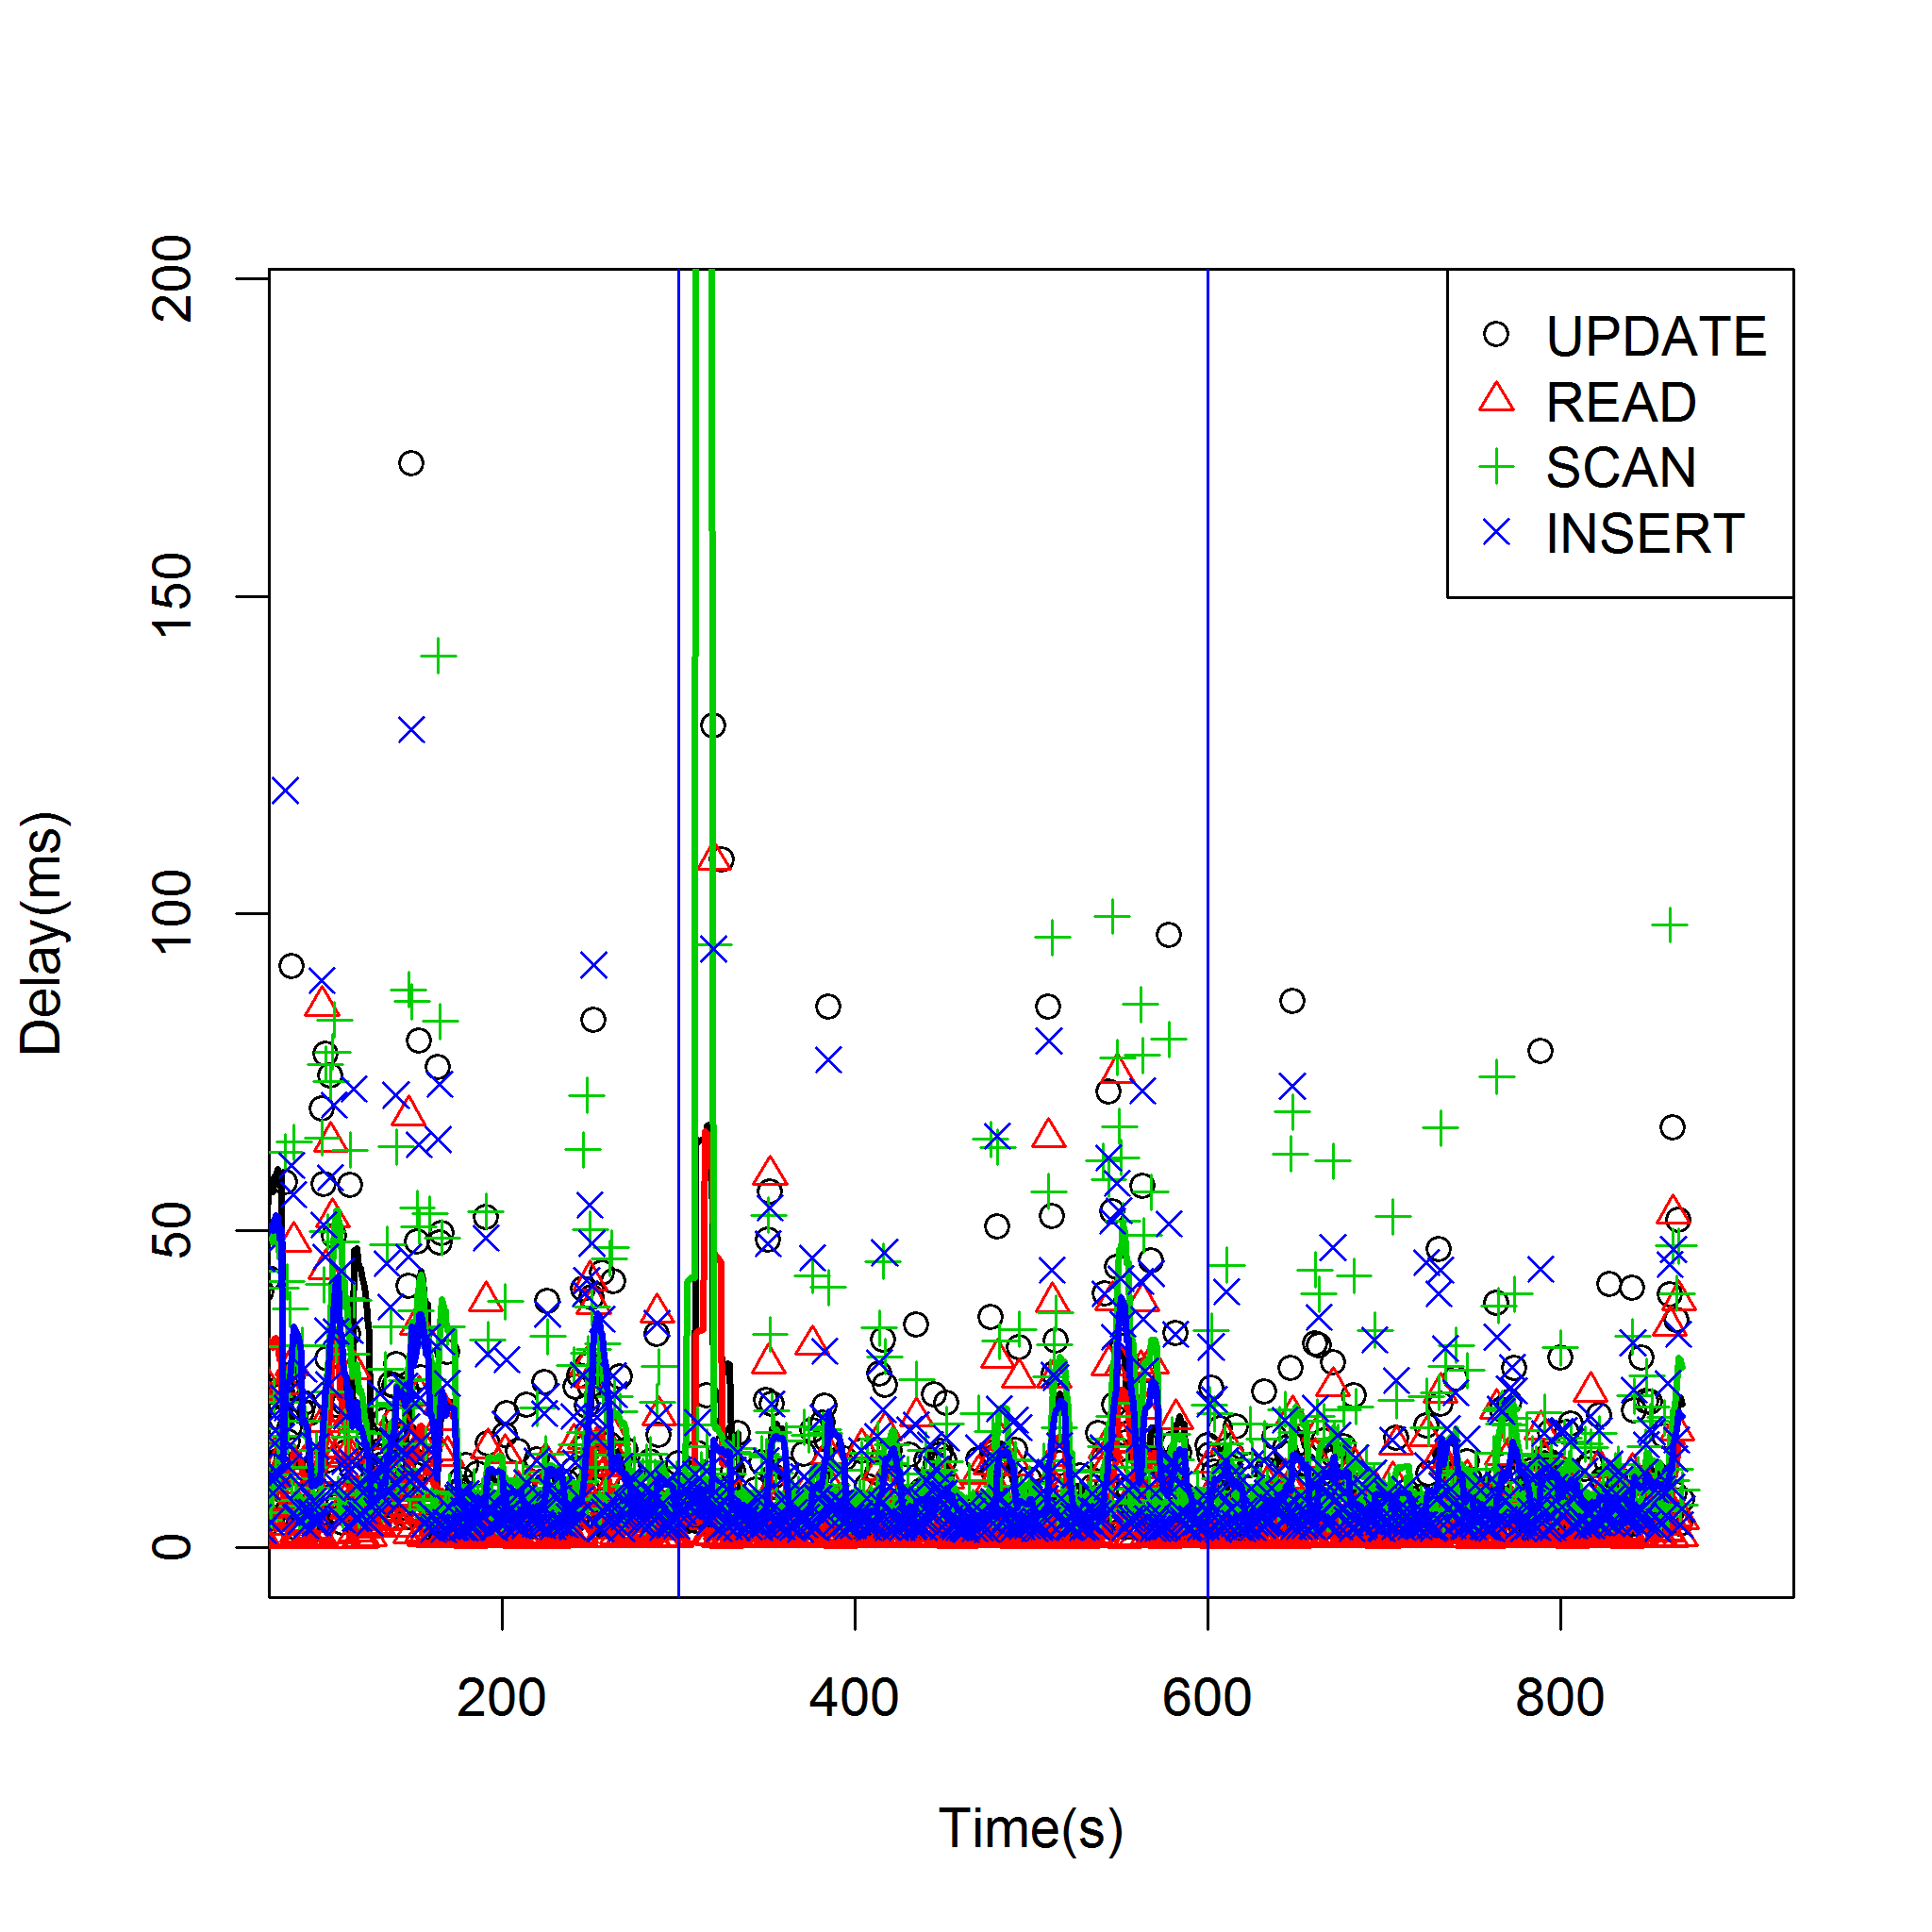
\includegraphics[width=0.9\textwidth]{img/Observaties/MongoDB/single-graph-6-1}}
	\subfigure{\label{fig:beschikbaar-mongodb-soft-zoom} 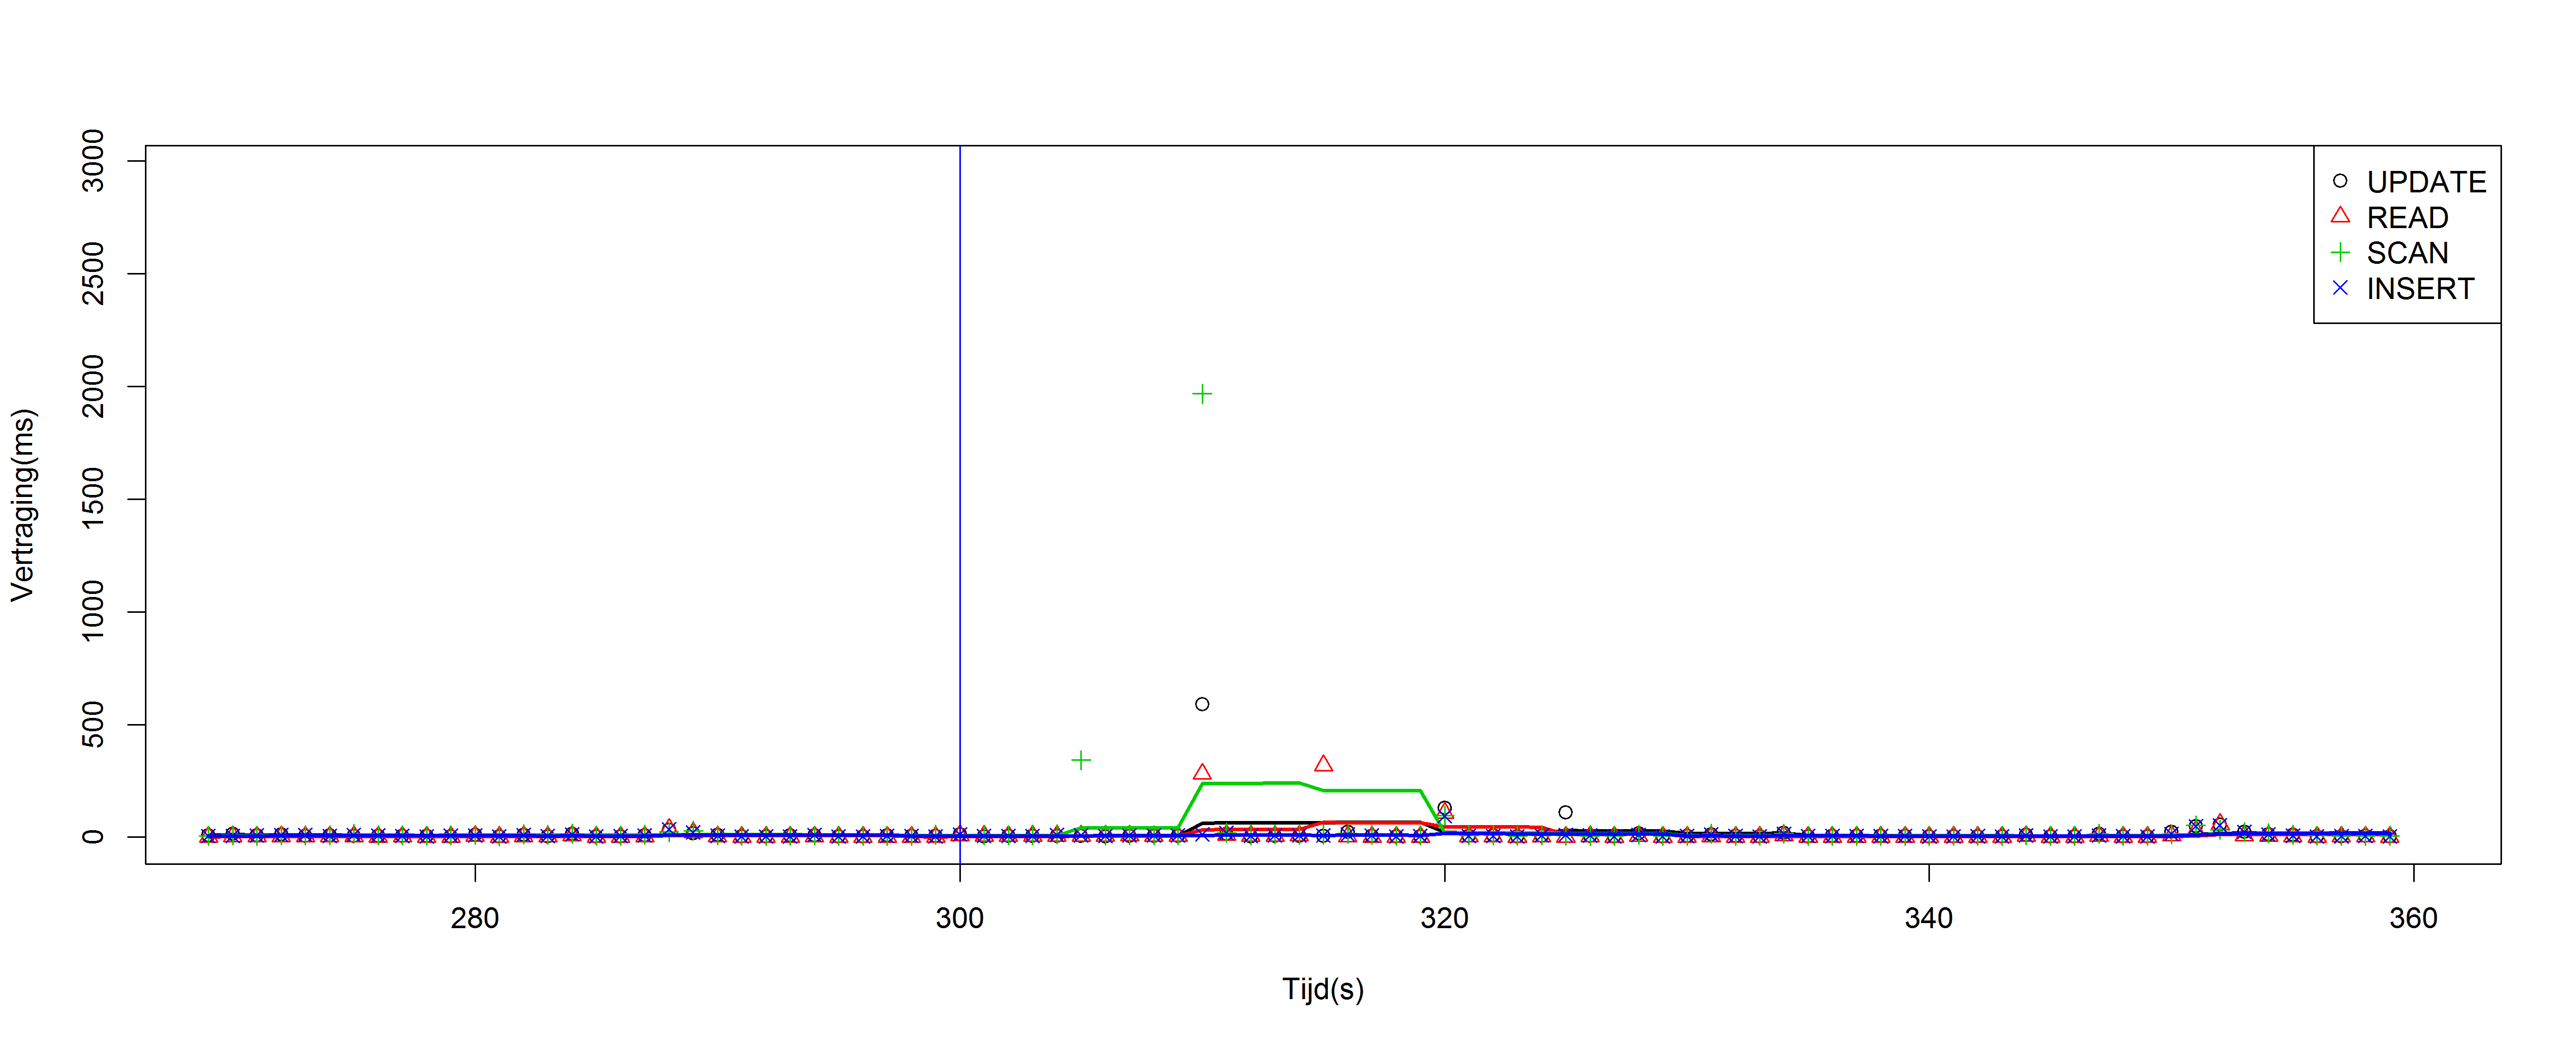
\includegraphics[width=0.9\textwidth]{img/Observaties/MongoDB/multiple-graph-interrupt-Node-6-Shut-down}}
	\subfigure{\label{fig:beschikbaar-mongodb-drop} 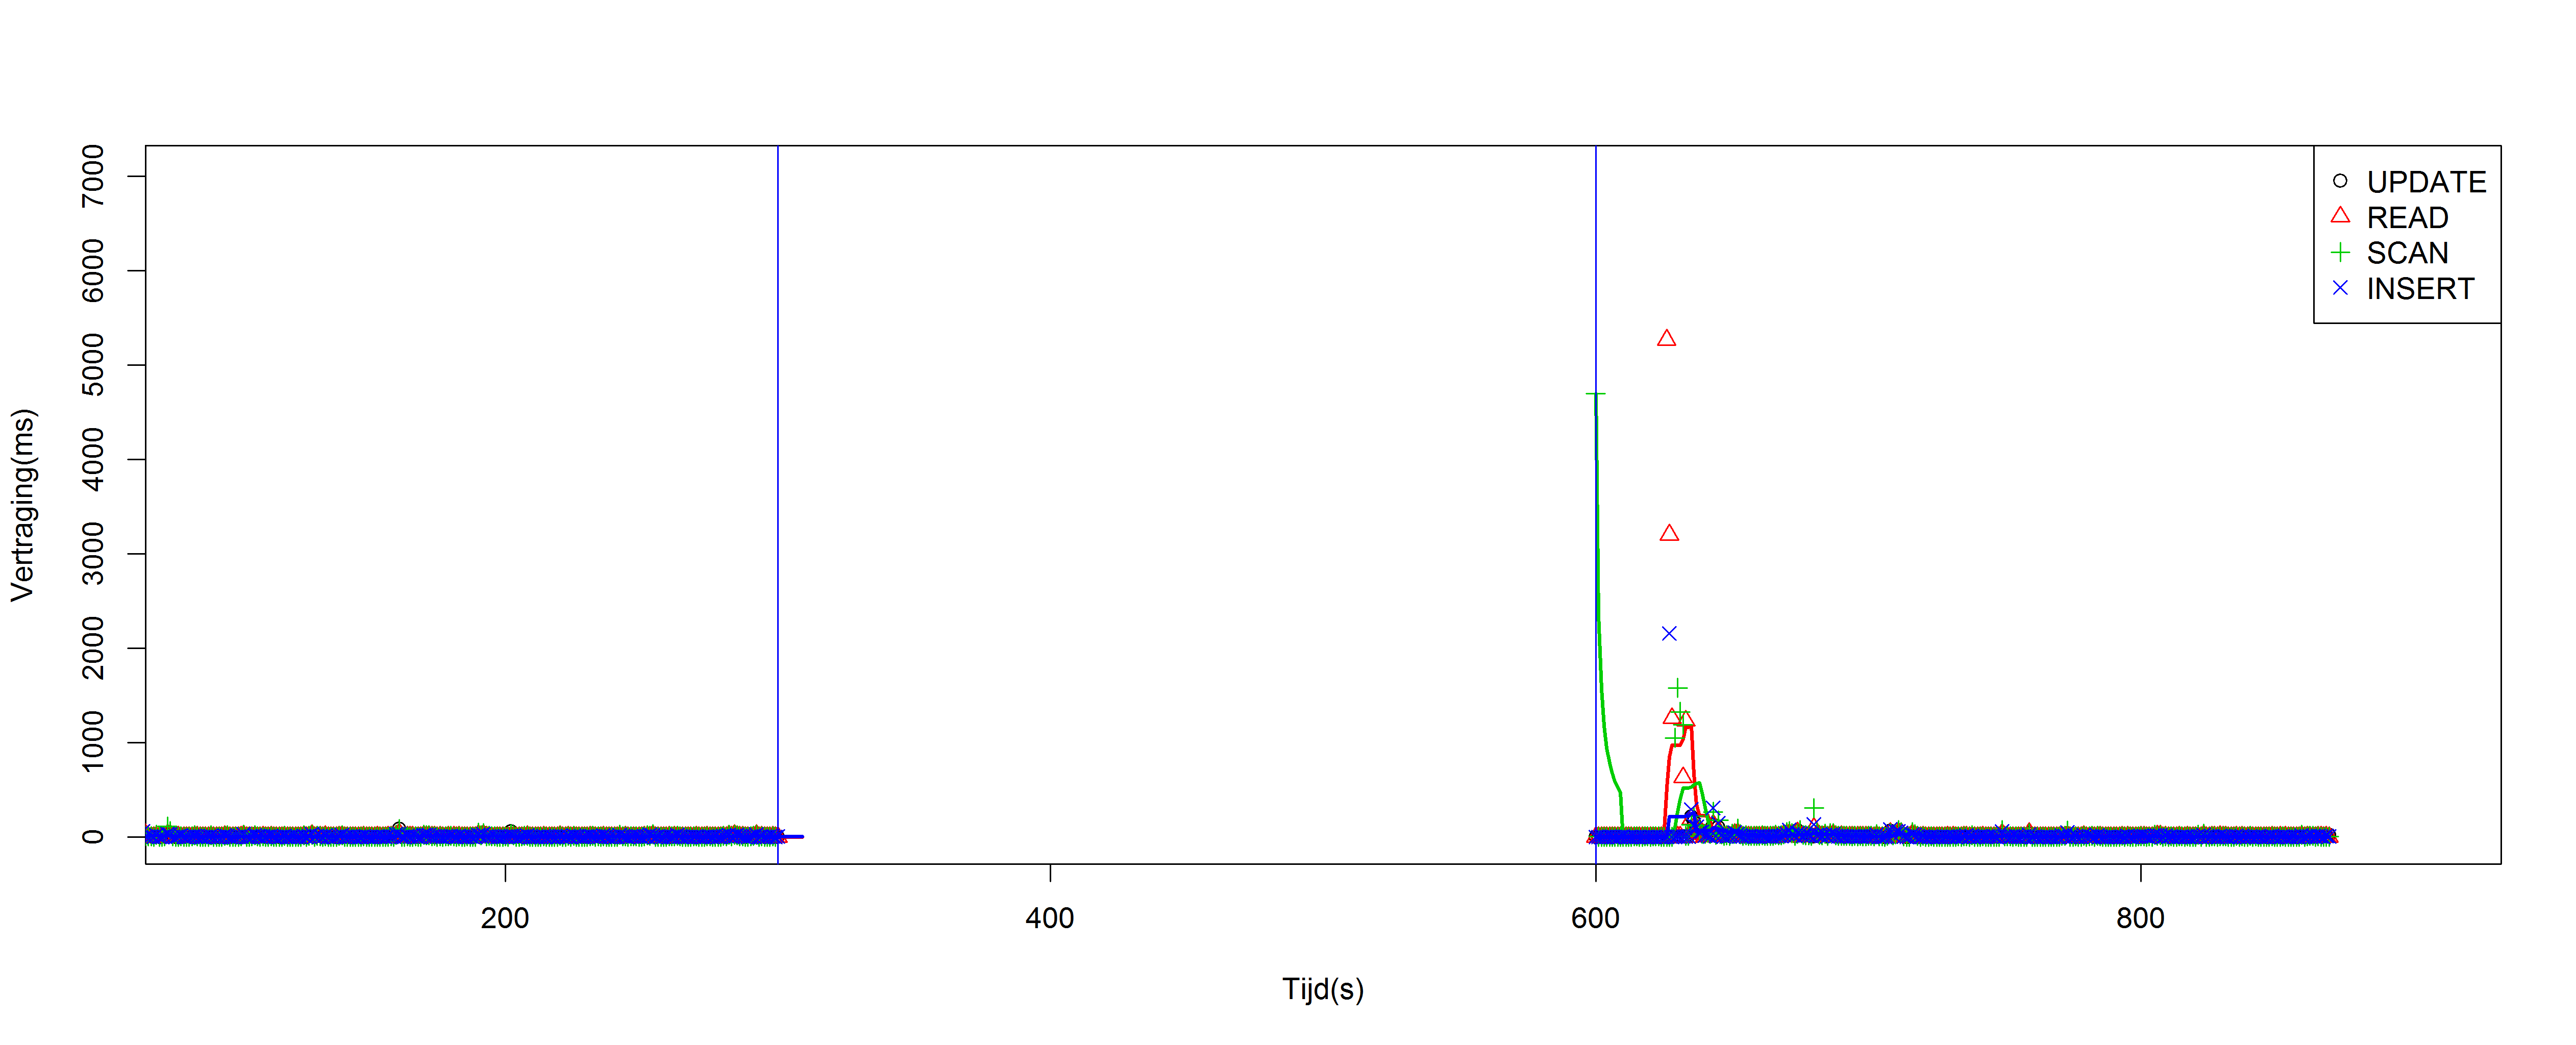
\includegraphics[width=0.9\textwidth]{img/Observaties/MongoDB/single-graph-4-drop-1}}
	\caption{\textbf{Beschikbaarheid van MongoDB} \newline
	MongoDB heeft verschillende reacties op het stopzetten bij standaard configuratie van de queries (normaal schrijven en lezen van de primary). In het geval van zacht of hard stoppen is er geen verschil in de reactie, bij 2/3 van de keren is er geen verschil merkbaar, bij 1/3 van de keren is er tijdelijke verhoging van de vertraging. Een voorbeeld toont dat de scan operatie voor 2 seconden uitgesteld wordt. De eerste figuur is een overzicht, de middelste illustreert een zoom naar de stop.\newline
	Bij het onderbreken van het netwerk is er in bepaalde gevallen geen significante verandering, op andere momenten is een gedrag soortgelijk aan dat bij een zachte stop op te merken. In andere gevallen is het zo dat er geen queries mogelijk zijn gedurende de volledige netwerk onderbreking (zie de derde figuur) \newline
	Tijdens de onderbreking (400s- 500s), is er geen significante verandering in de vertraging van de uitgevoerde queries gemeten (t.o.v. 150-250s en 700s - 800s). \newline
	 }
	\label{fig:beschikbaar-mongodb-1}
\end{figure}

\begin{figure}[ht!] 
	\centering
	\subfigure{\label{fig:beschikbaar-pgpool-soft} 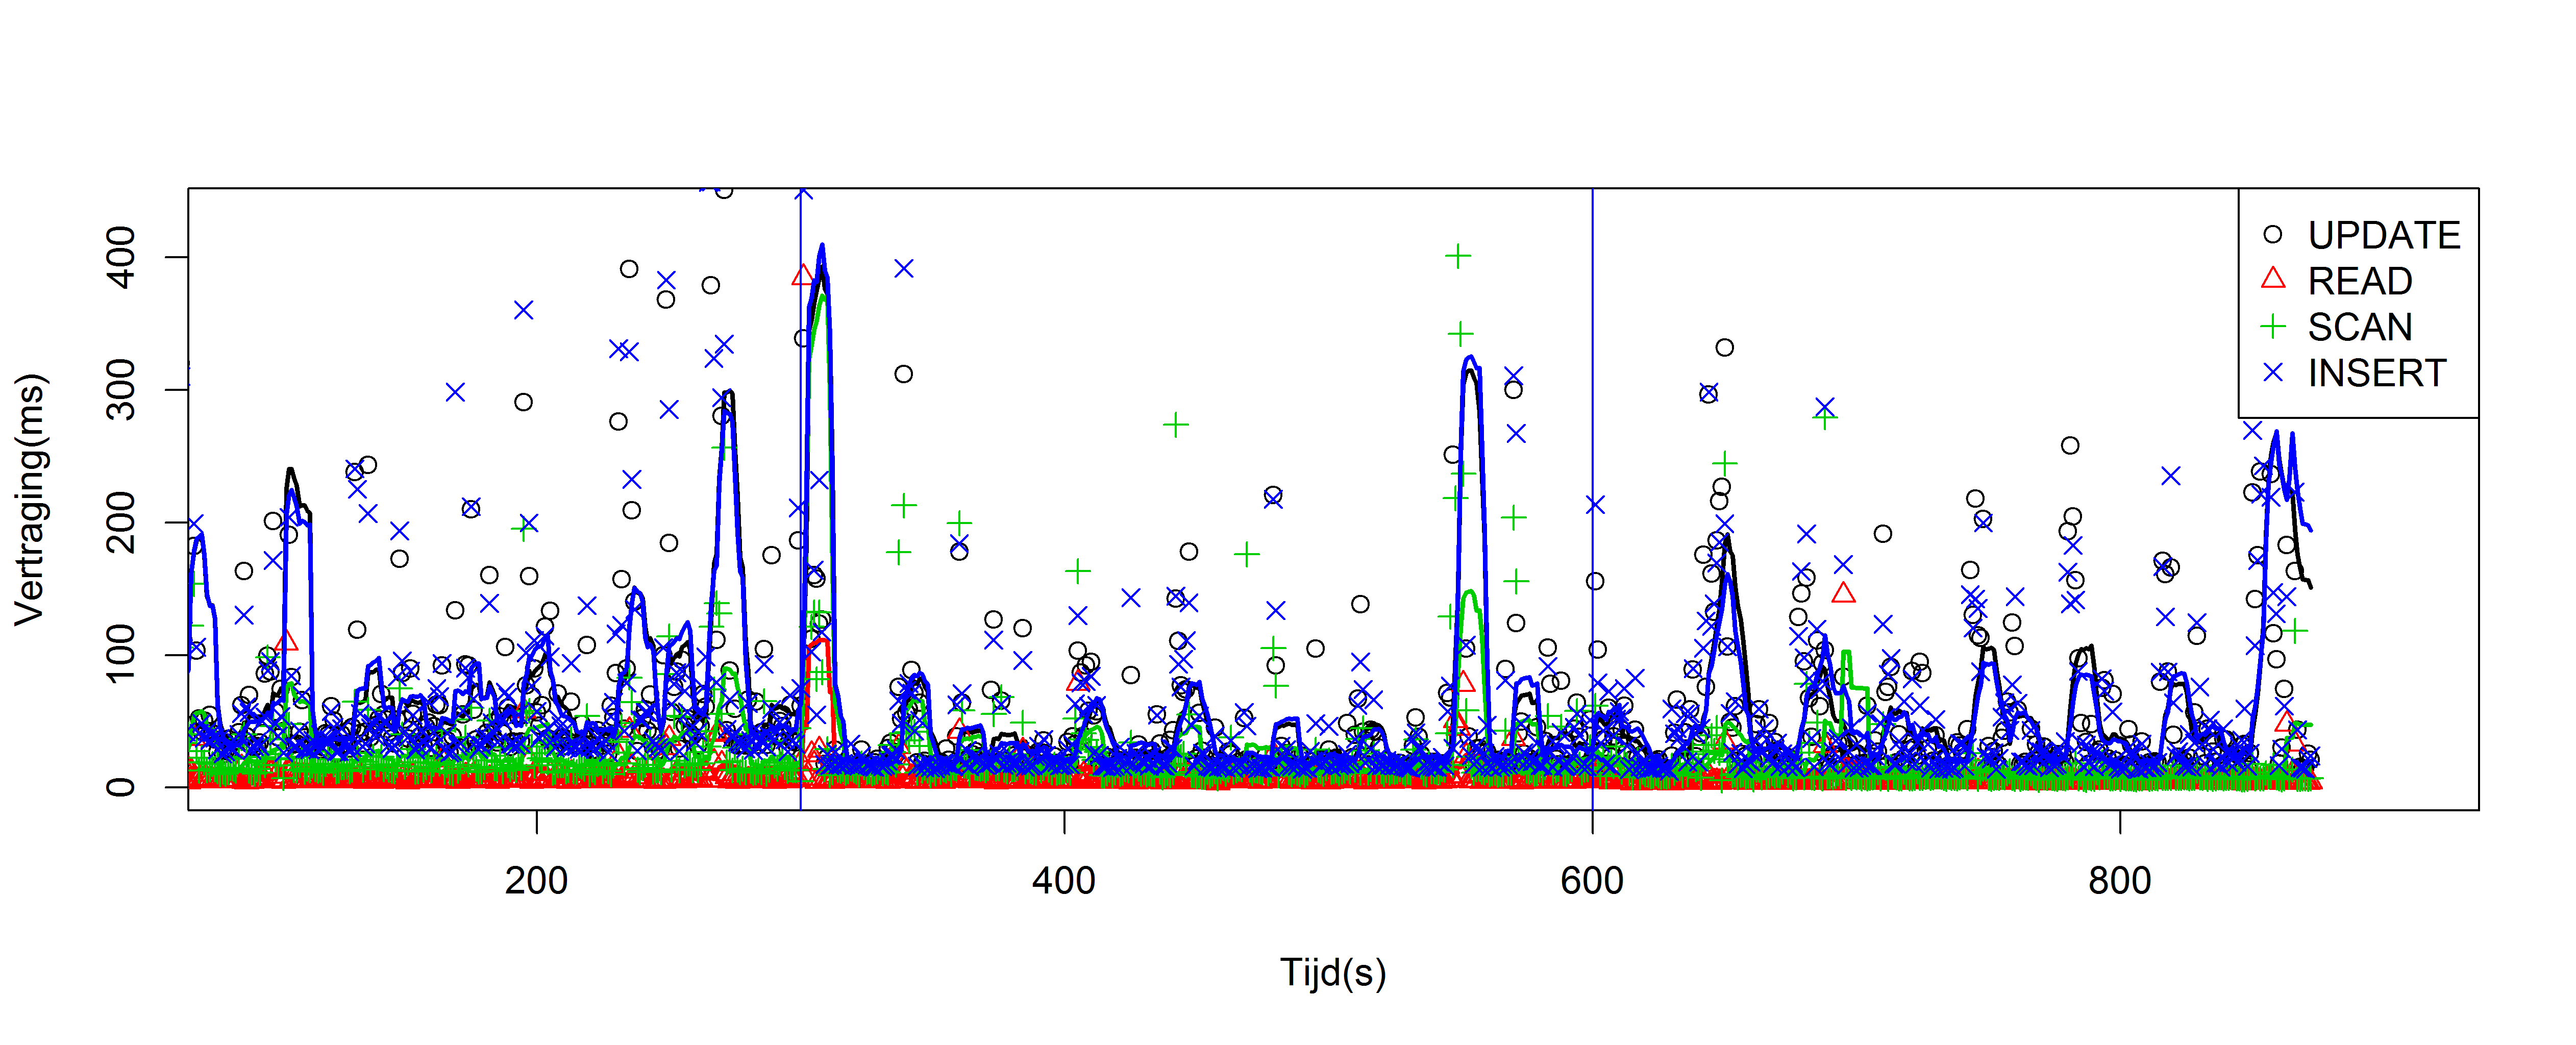
\includegraphics[width=0.95\textwidth]{img/Observaties/Pgpool/single-graph-1-2}}
	\subfigure{\label{fig:beschikbaar-pgpool-netwerk} 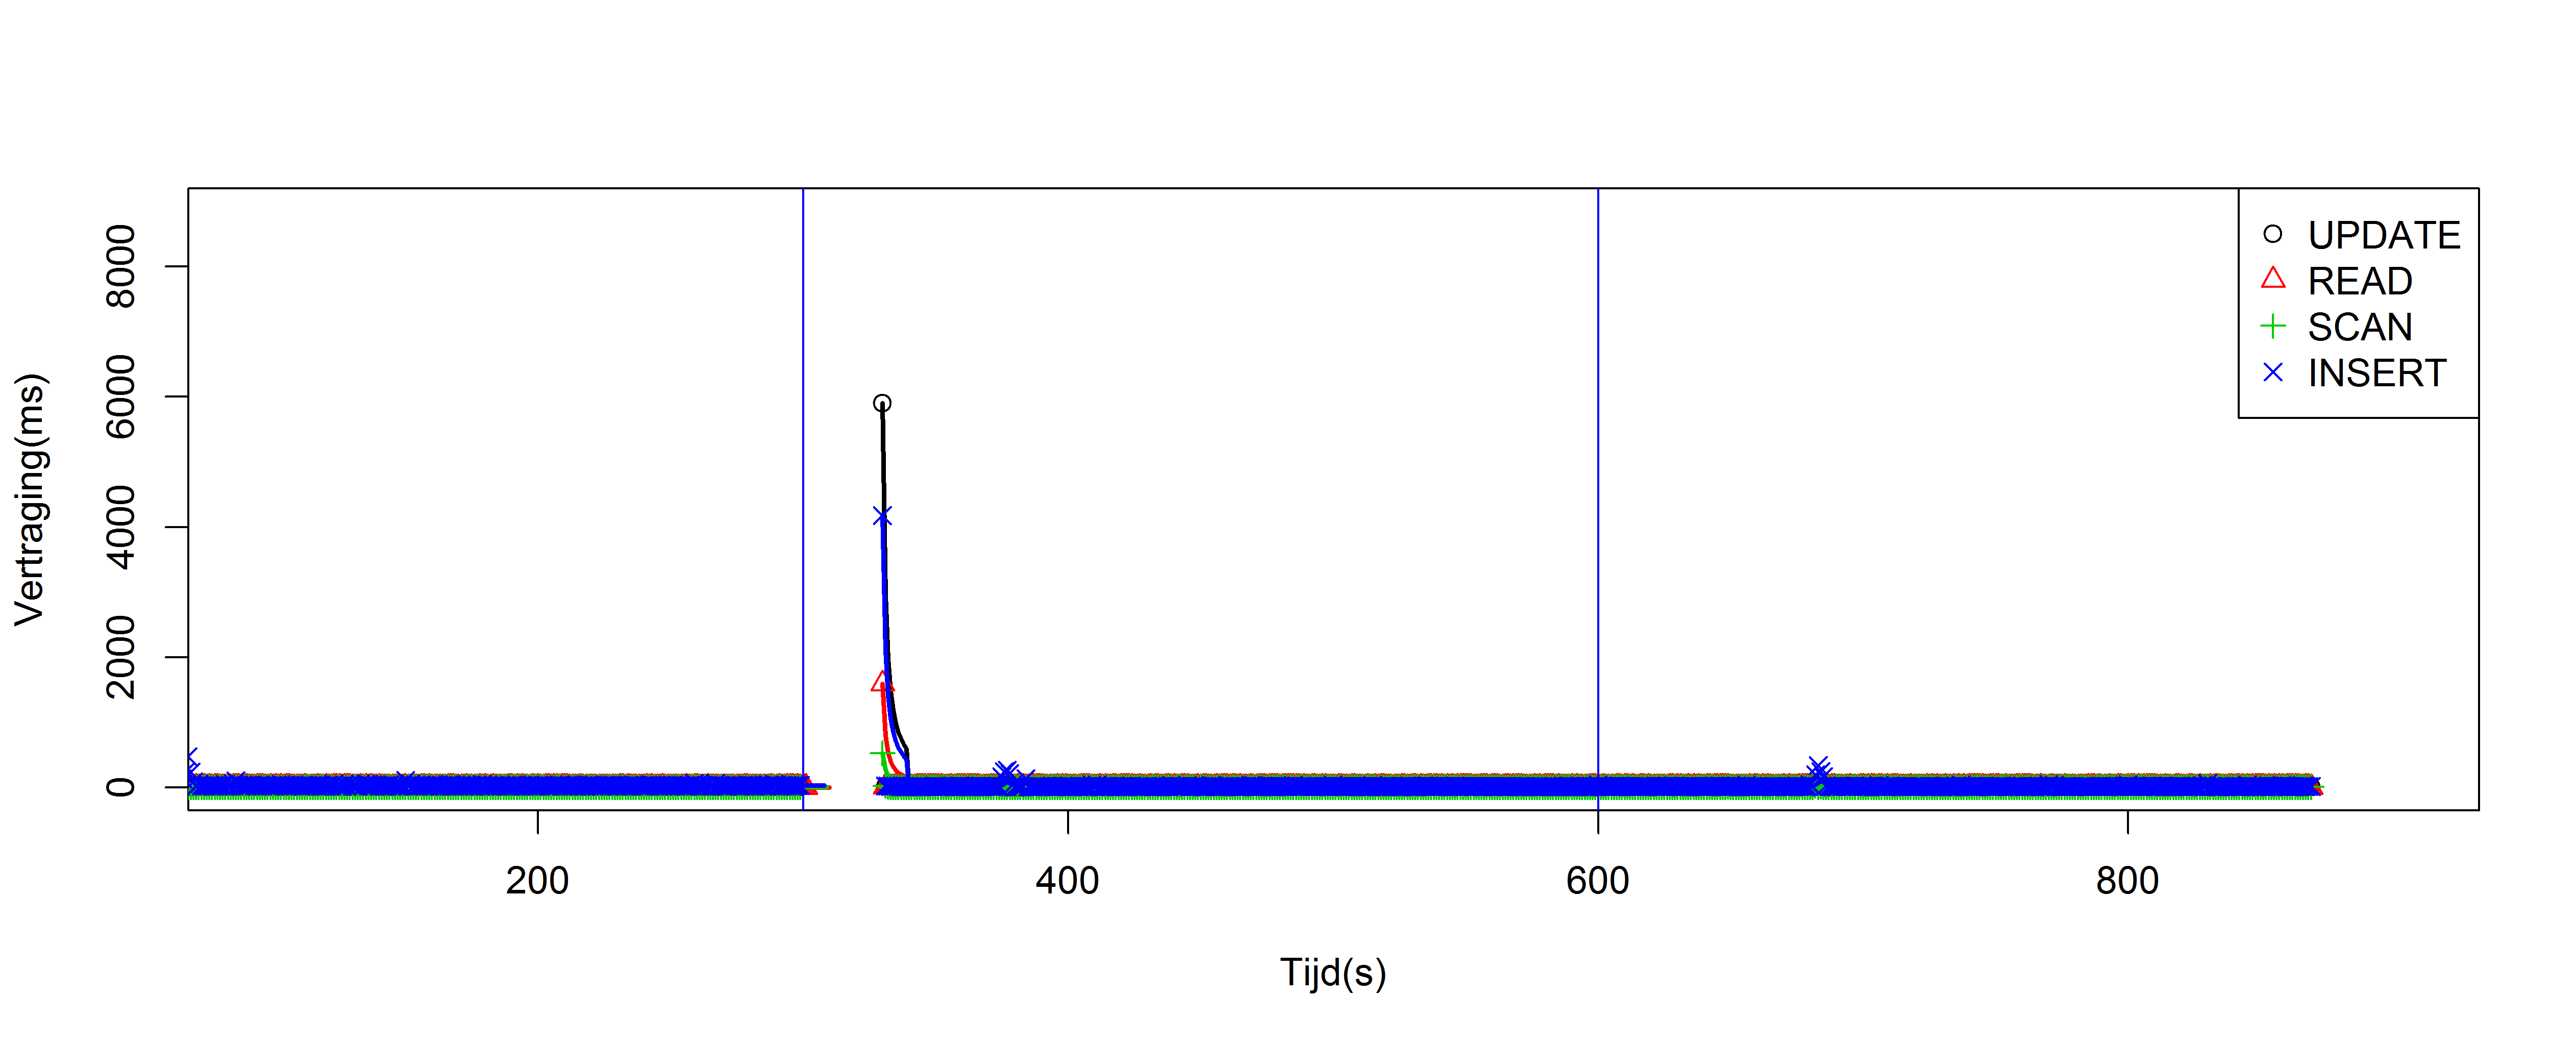
\includegraphics[width=0.95\textwidth]{img/Observaties/Pgpool/single-graph-1-drop-1}}
	\subfigure[Boxplot met leesvertragingen]{\label{fig:beschikbaar-pgpool-boxplot-read} 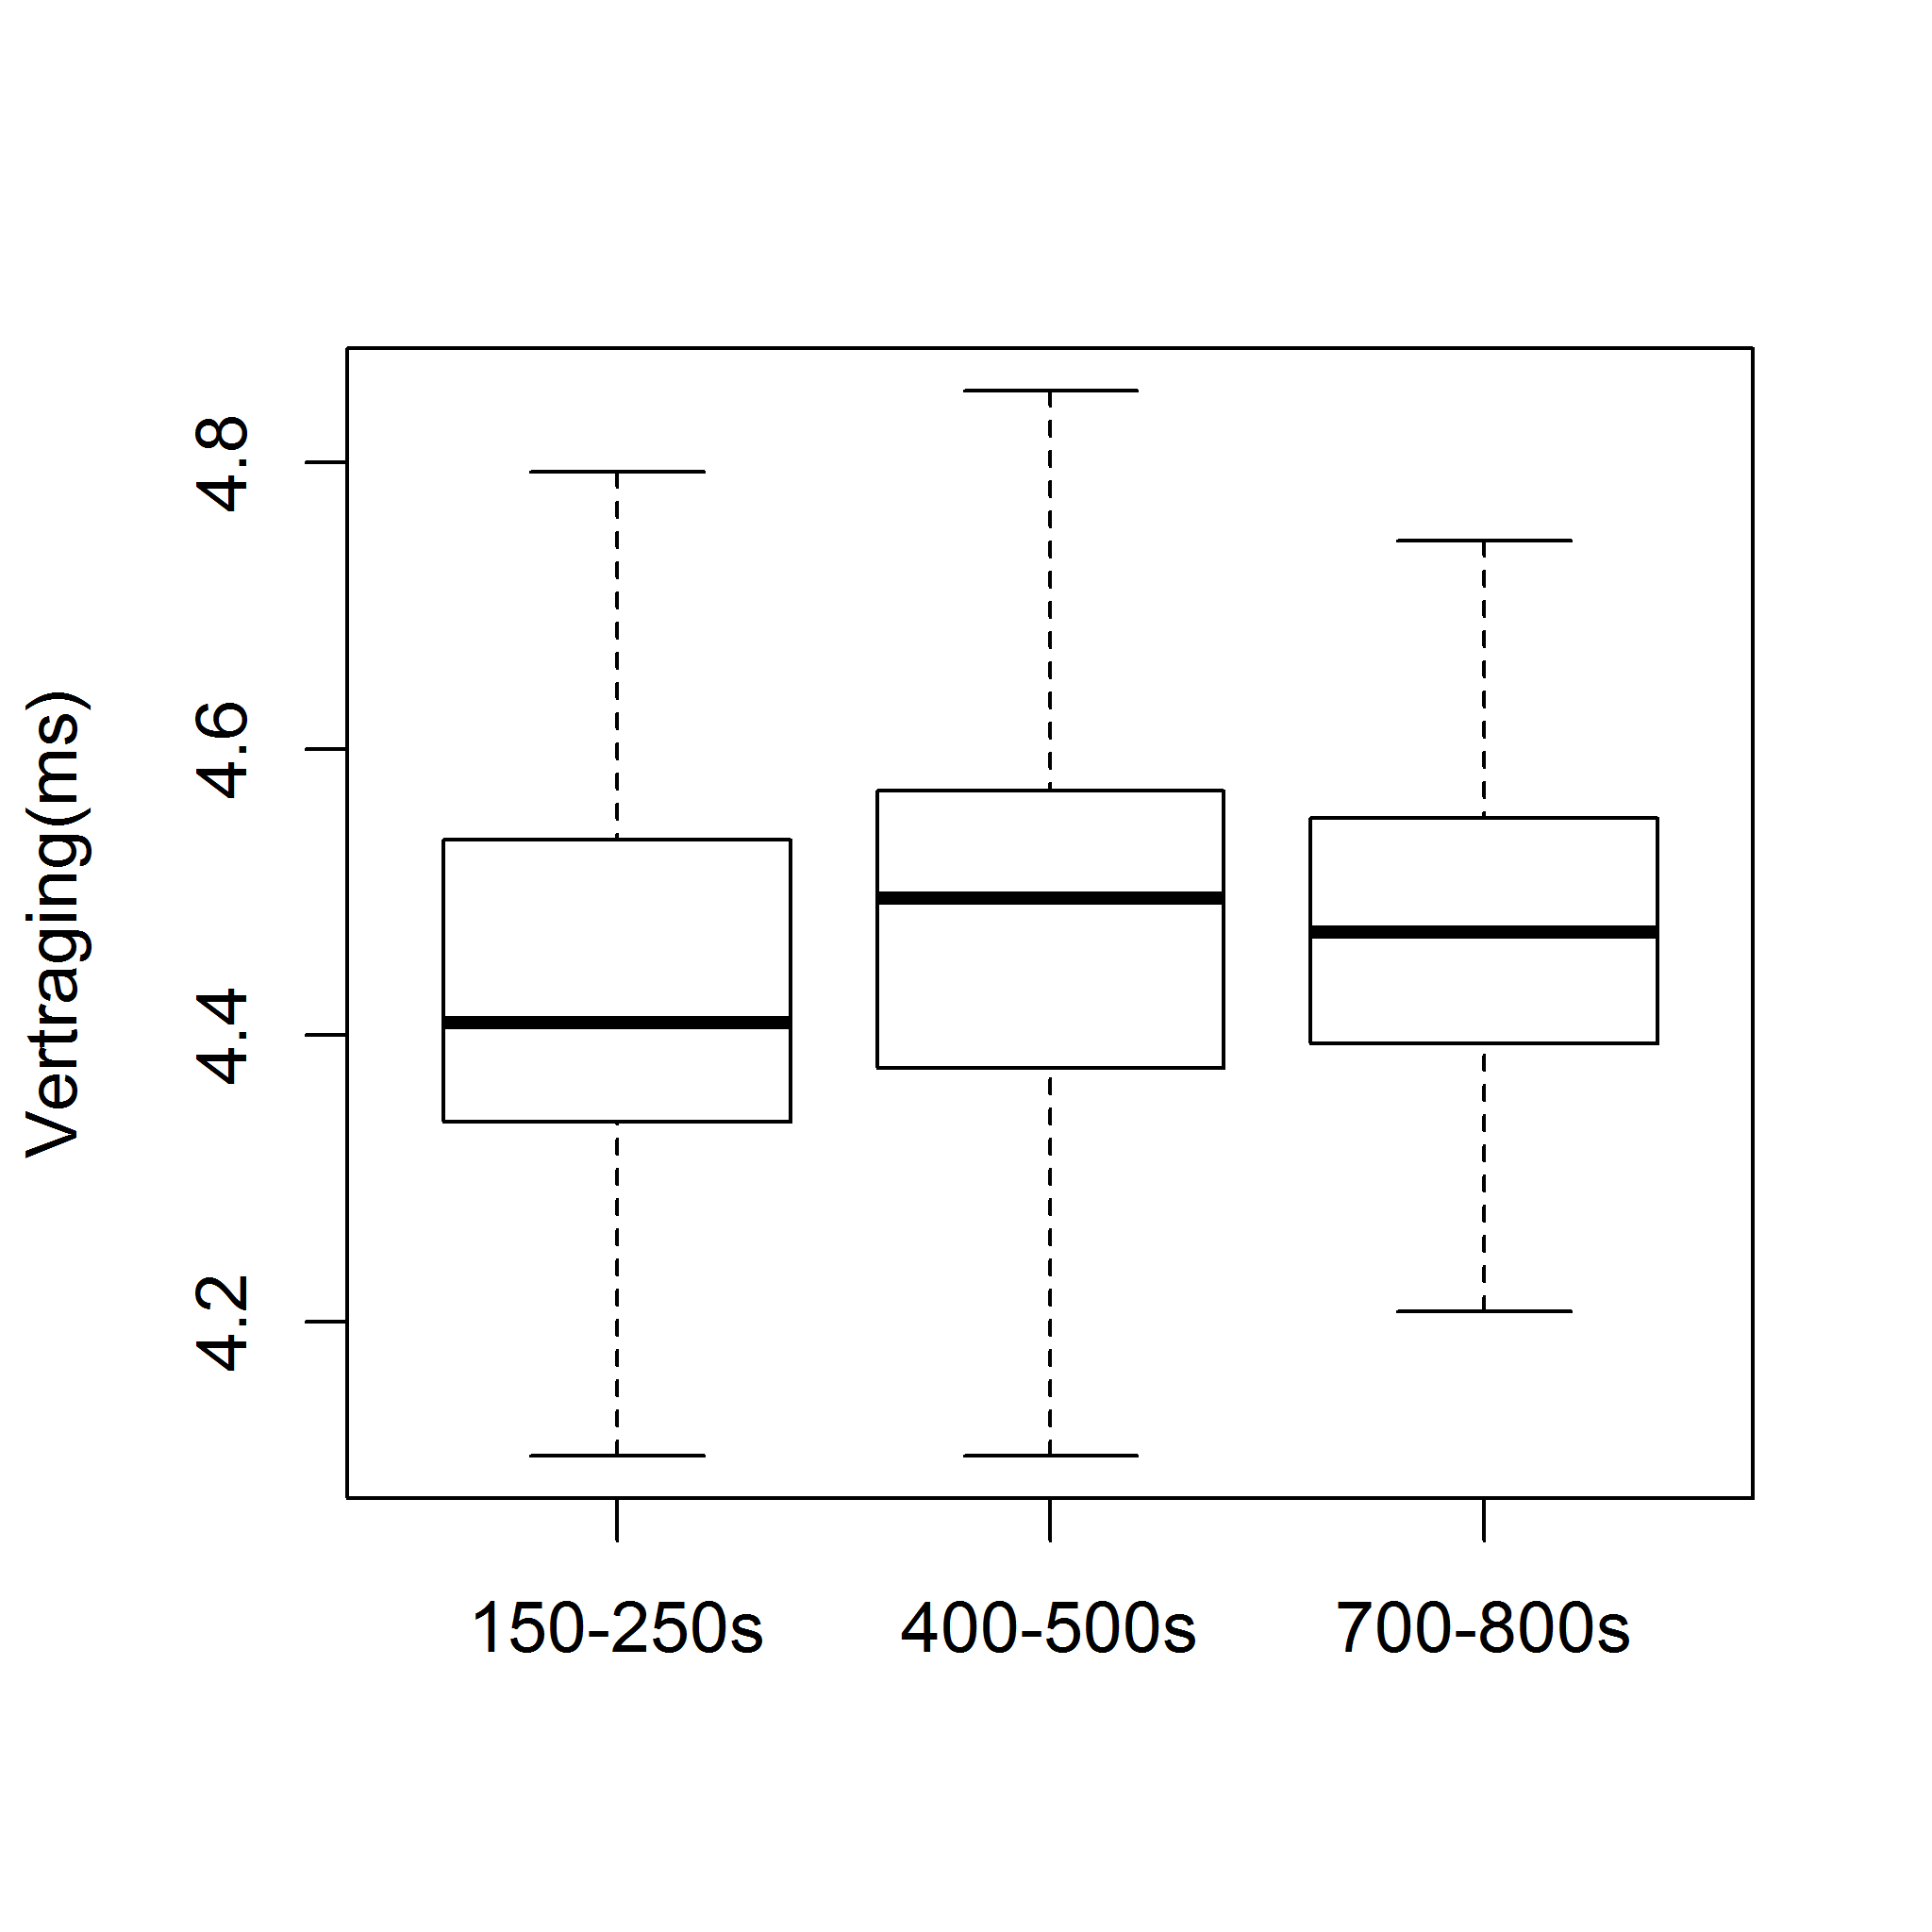
\includegraphics[width=0.45\textwidth]{img/Observaties/Pgpool/boxplot-graph-Node-1-READ}}
	\subfigure[Boxplot met schrijf vertragingen]{\label{fig:beschikbaar-pgpool-boxplot-write} 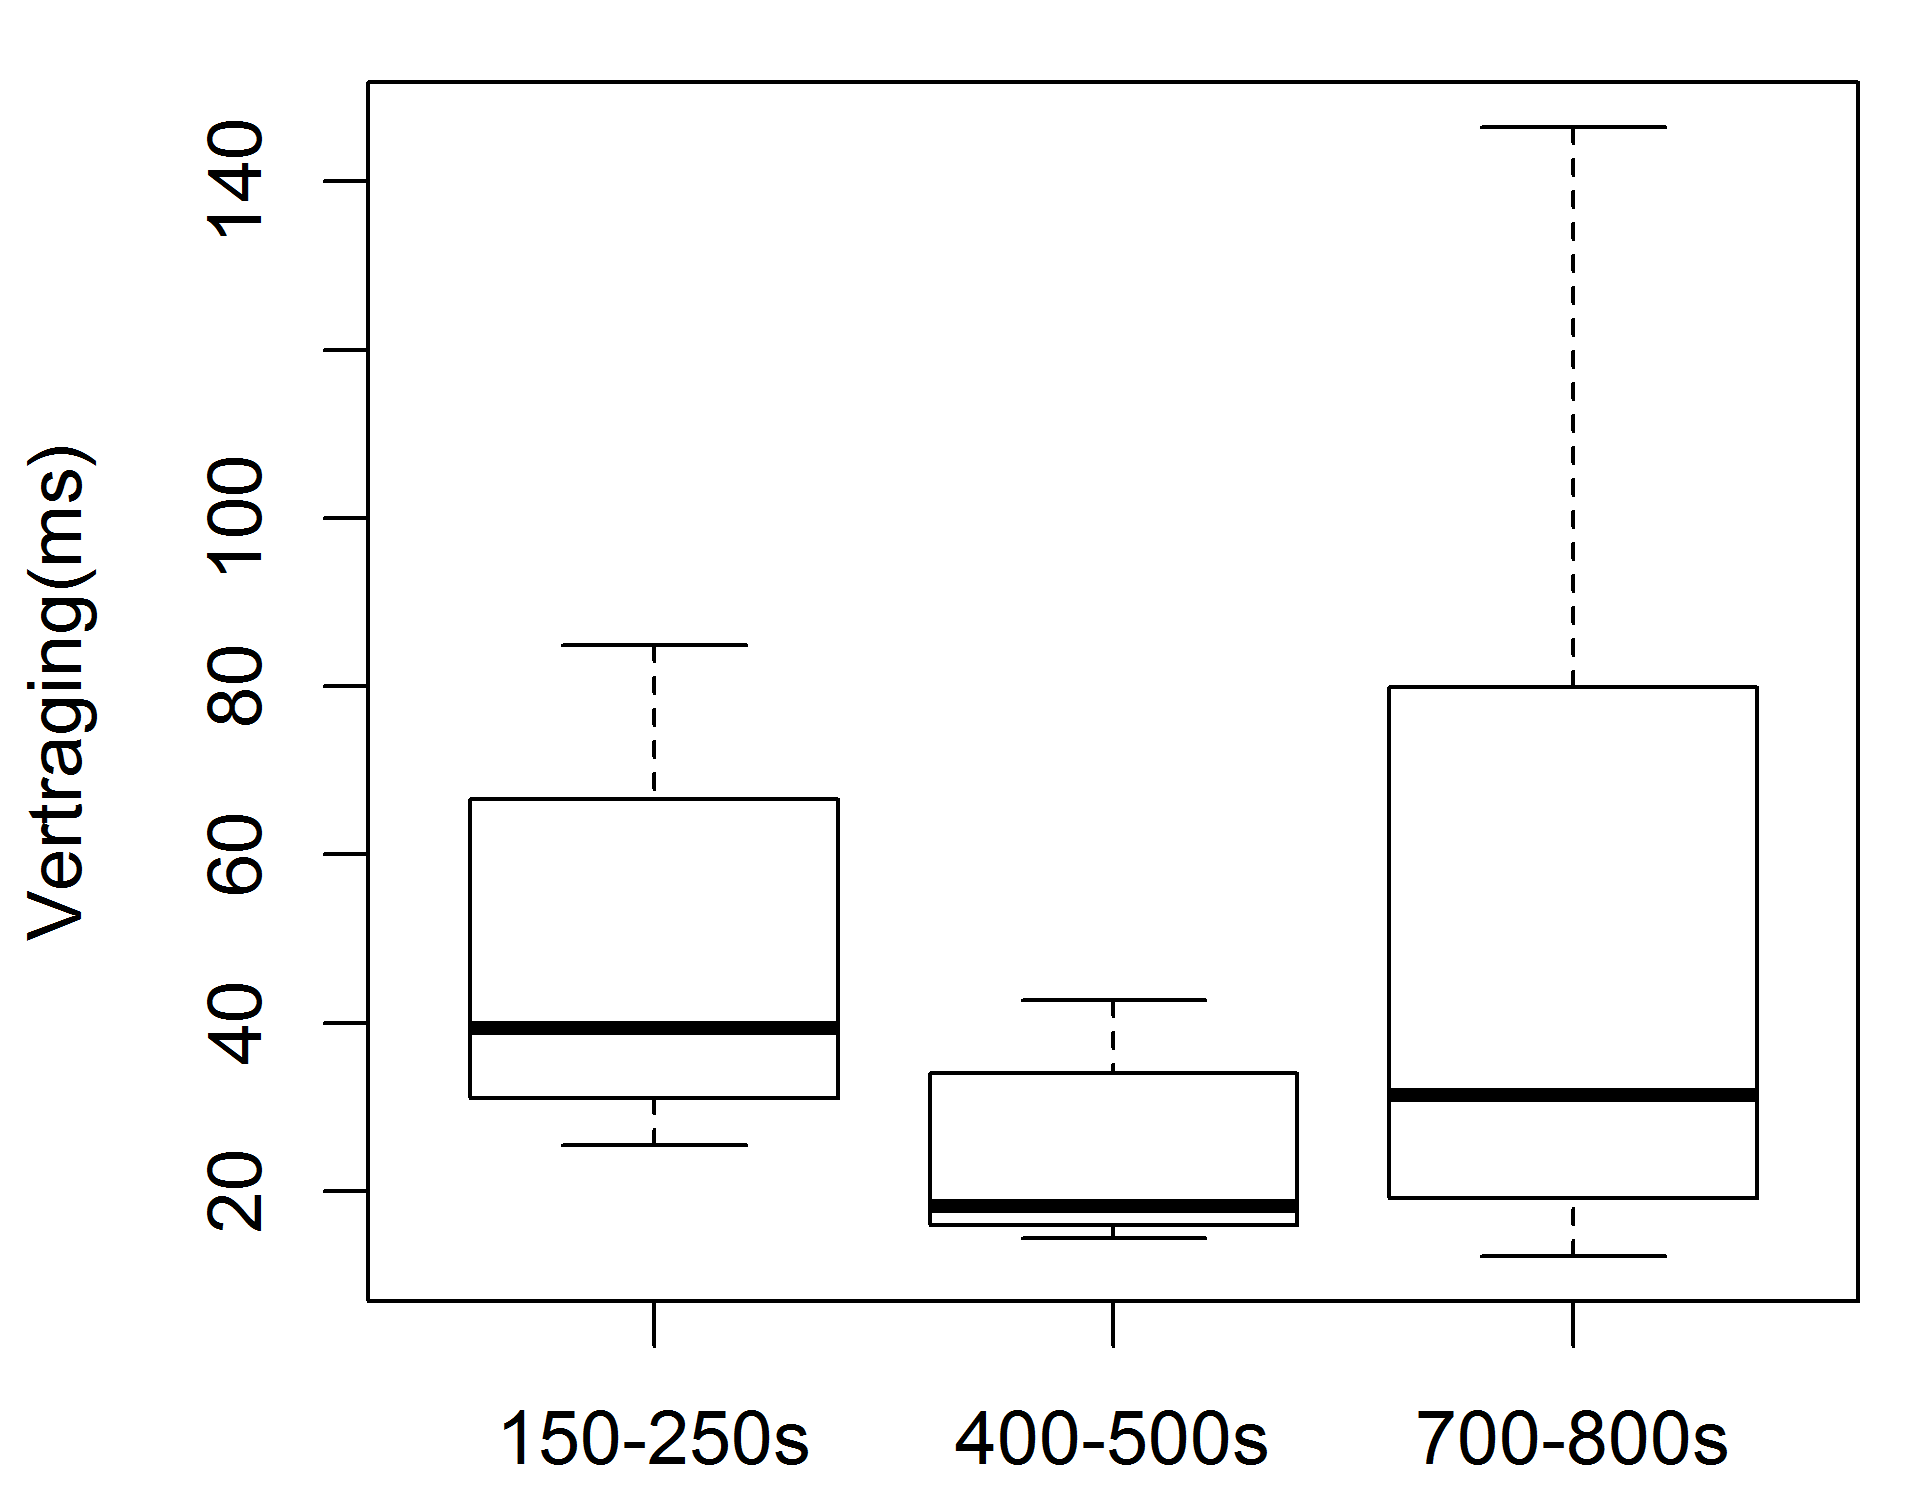
\includegraphics[width=0.45\textwidth]{img/Observaties/Pgpool/boxplot-graph-Node-1-UPDATE}}
	\caption{\textbf{Beschikbaarheid van Pgpool-II}\newline
	Bij Pgpool-II is een geen verschil tussen een harde of zachte stop. In beide gevallen is er tijdelijk een onderbreking van al de queries. Er is een verhoogde vertraging van ongeveer 2 seconden, een voorbeeld bevindt zich in de bovenste figuur. \newline
	Bij een netwerk onderbreking, zijn er enige tijd geen queries mogelijk en na 30 seconden is de onderbreking voorbij. Een voorbeeld bevindt zich in de middelste figuur.  \newline
	Tijdens de onderbreking is er een verandering van de vertraging van de schrijfbewerkingen: deze nemen significant minder tijd in beslag. Dit geldt niet voor leesbewerkingen. Voorbeelden uit de testen bevinden zich voor beiden in figuren (c) en (d). \newline
	Het herstel van een server nadat deze opnieuw online gebracht hebben, lukt niet tijdens de testen. Enkel als alle connecties verbroken zijn, wat het geval is na de testen, slaagt het herstel.  }
	\label{fig:beschikbaar-pgpool}
\end{figure}

\FloatBarrier
\section{Consistentietest}
Voor de consistentietesten worden er twee soorten grafieken gebruikt. Het meest gebruikt zijn de empirische verdelingsfuncties.  Dit zijn functies waarbij op de y-as het percentage staat van de waarden kleiner dan x.

Voor de consistentie testen wordt er op de x-as de start- en/of stoptijdstippen van de verschillende soorten getoond. Het verschil tussen de y-waarde van de start- en stoptijdstippen geeft aan hoeveel queries er op dat moment uitgevoerd worden. De getoonde tijdstippen van een lezer zijn de eerste keer dat deze de correcte data leest. 

De tweede soort figuren heeft op de x-as het sleutel nummer en op de y-as wordt de vertraging getoond. De grafieken die geplot worden zijn de het start- en eindtijdstip van zowel de schrijfbewerking als de verschillende pogingen van een bepaalde lezer. 

\begin{figure}[b] 
	\centering
	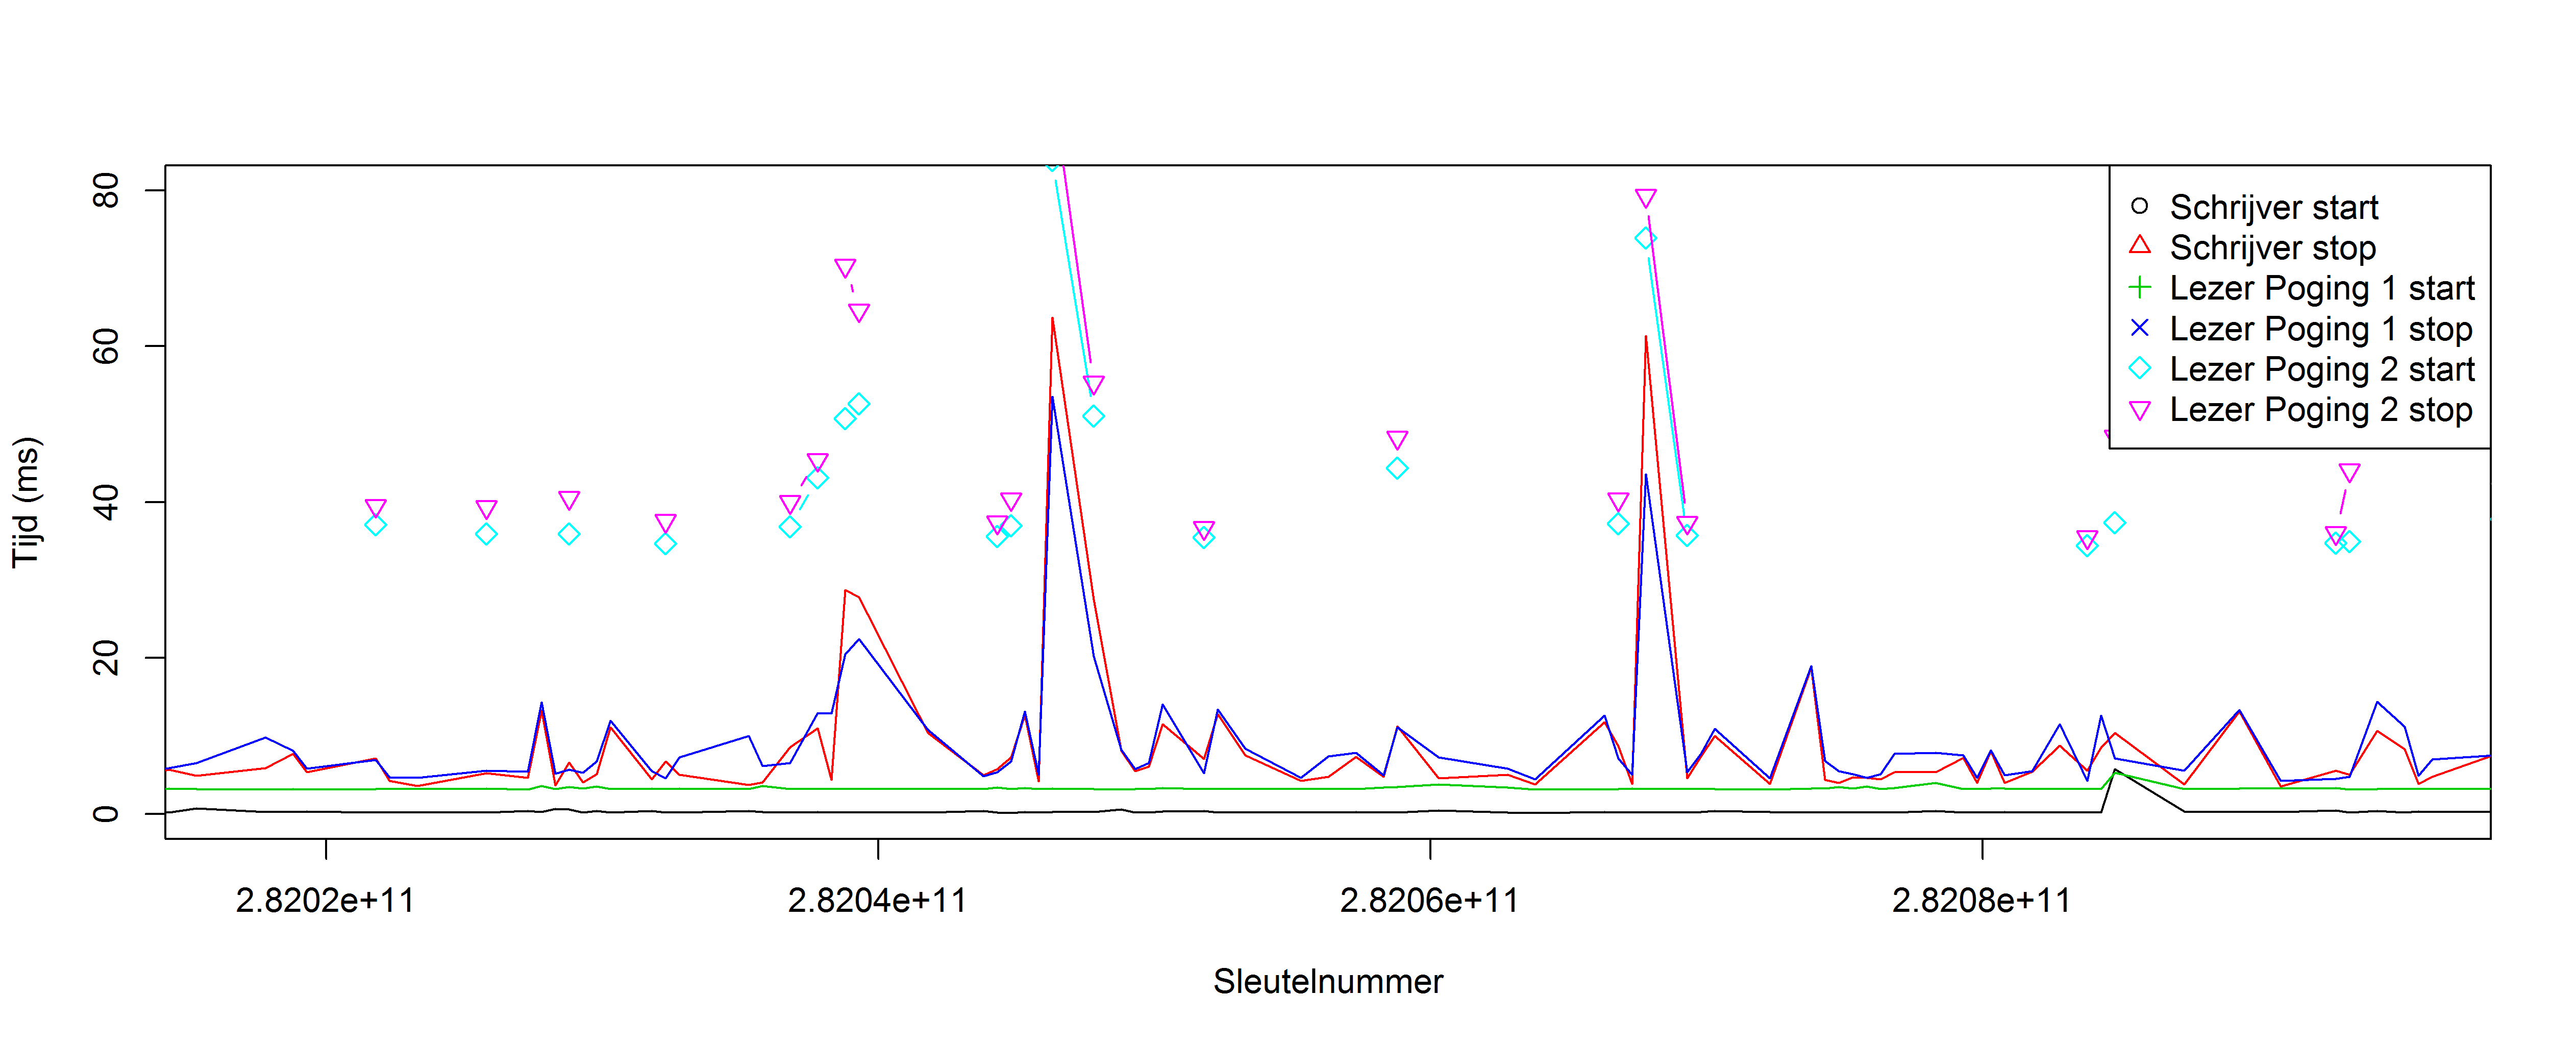
\includegraphics[width=\textwidth]{img/Observaties/HBase/consistency-plot-R-1-insertRawData-5}

	\caption{\textbf{Consistentie van HBase: Tijdsverloop} \newline
 	In de figuur zijn op de x-as verschillende pogingen doorheen de tijd voorgesteld. Op de y-as staat de vertraging voor elke bewerking. De lezer zal een tweede keer moeten lezen de eerste poging van de leesactie gedaan is voor de schrijfactie voltooid is. Ook volgt het einde van de leesactie het einde van de schrijfactie. }
	\label{fig:consistentie-hbase-tijdschaal-lezer-1}
\end{figure}

\begin{figure}[ht!] 
	\centering
	\subfigure{\label{fig:consistentie-hbase-start} 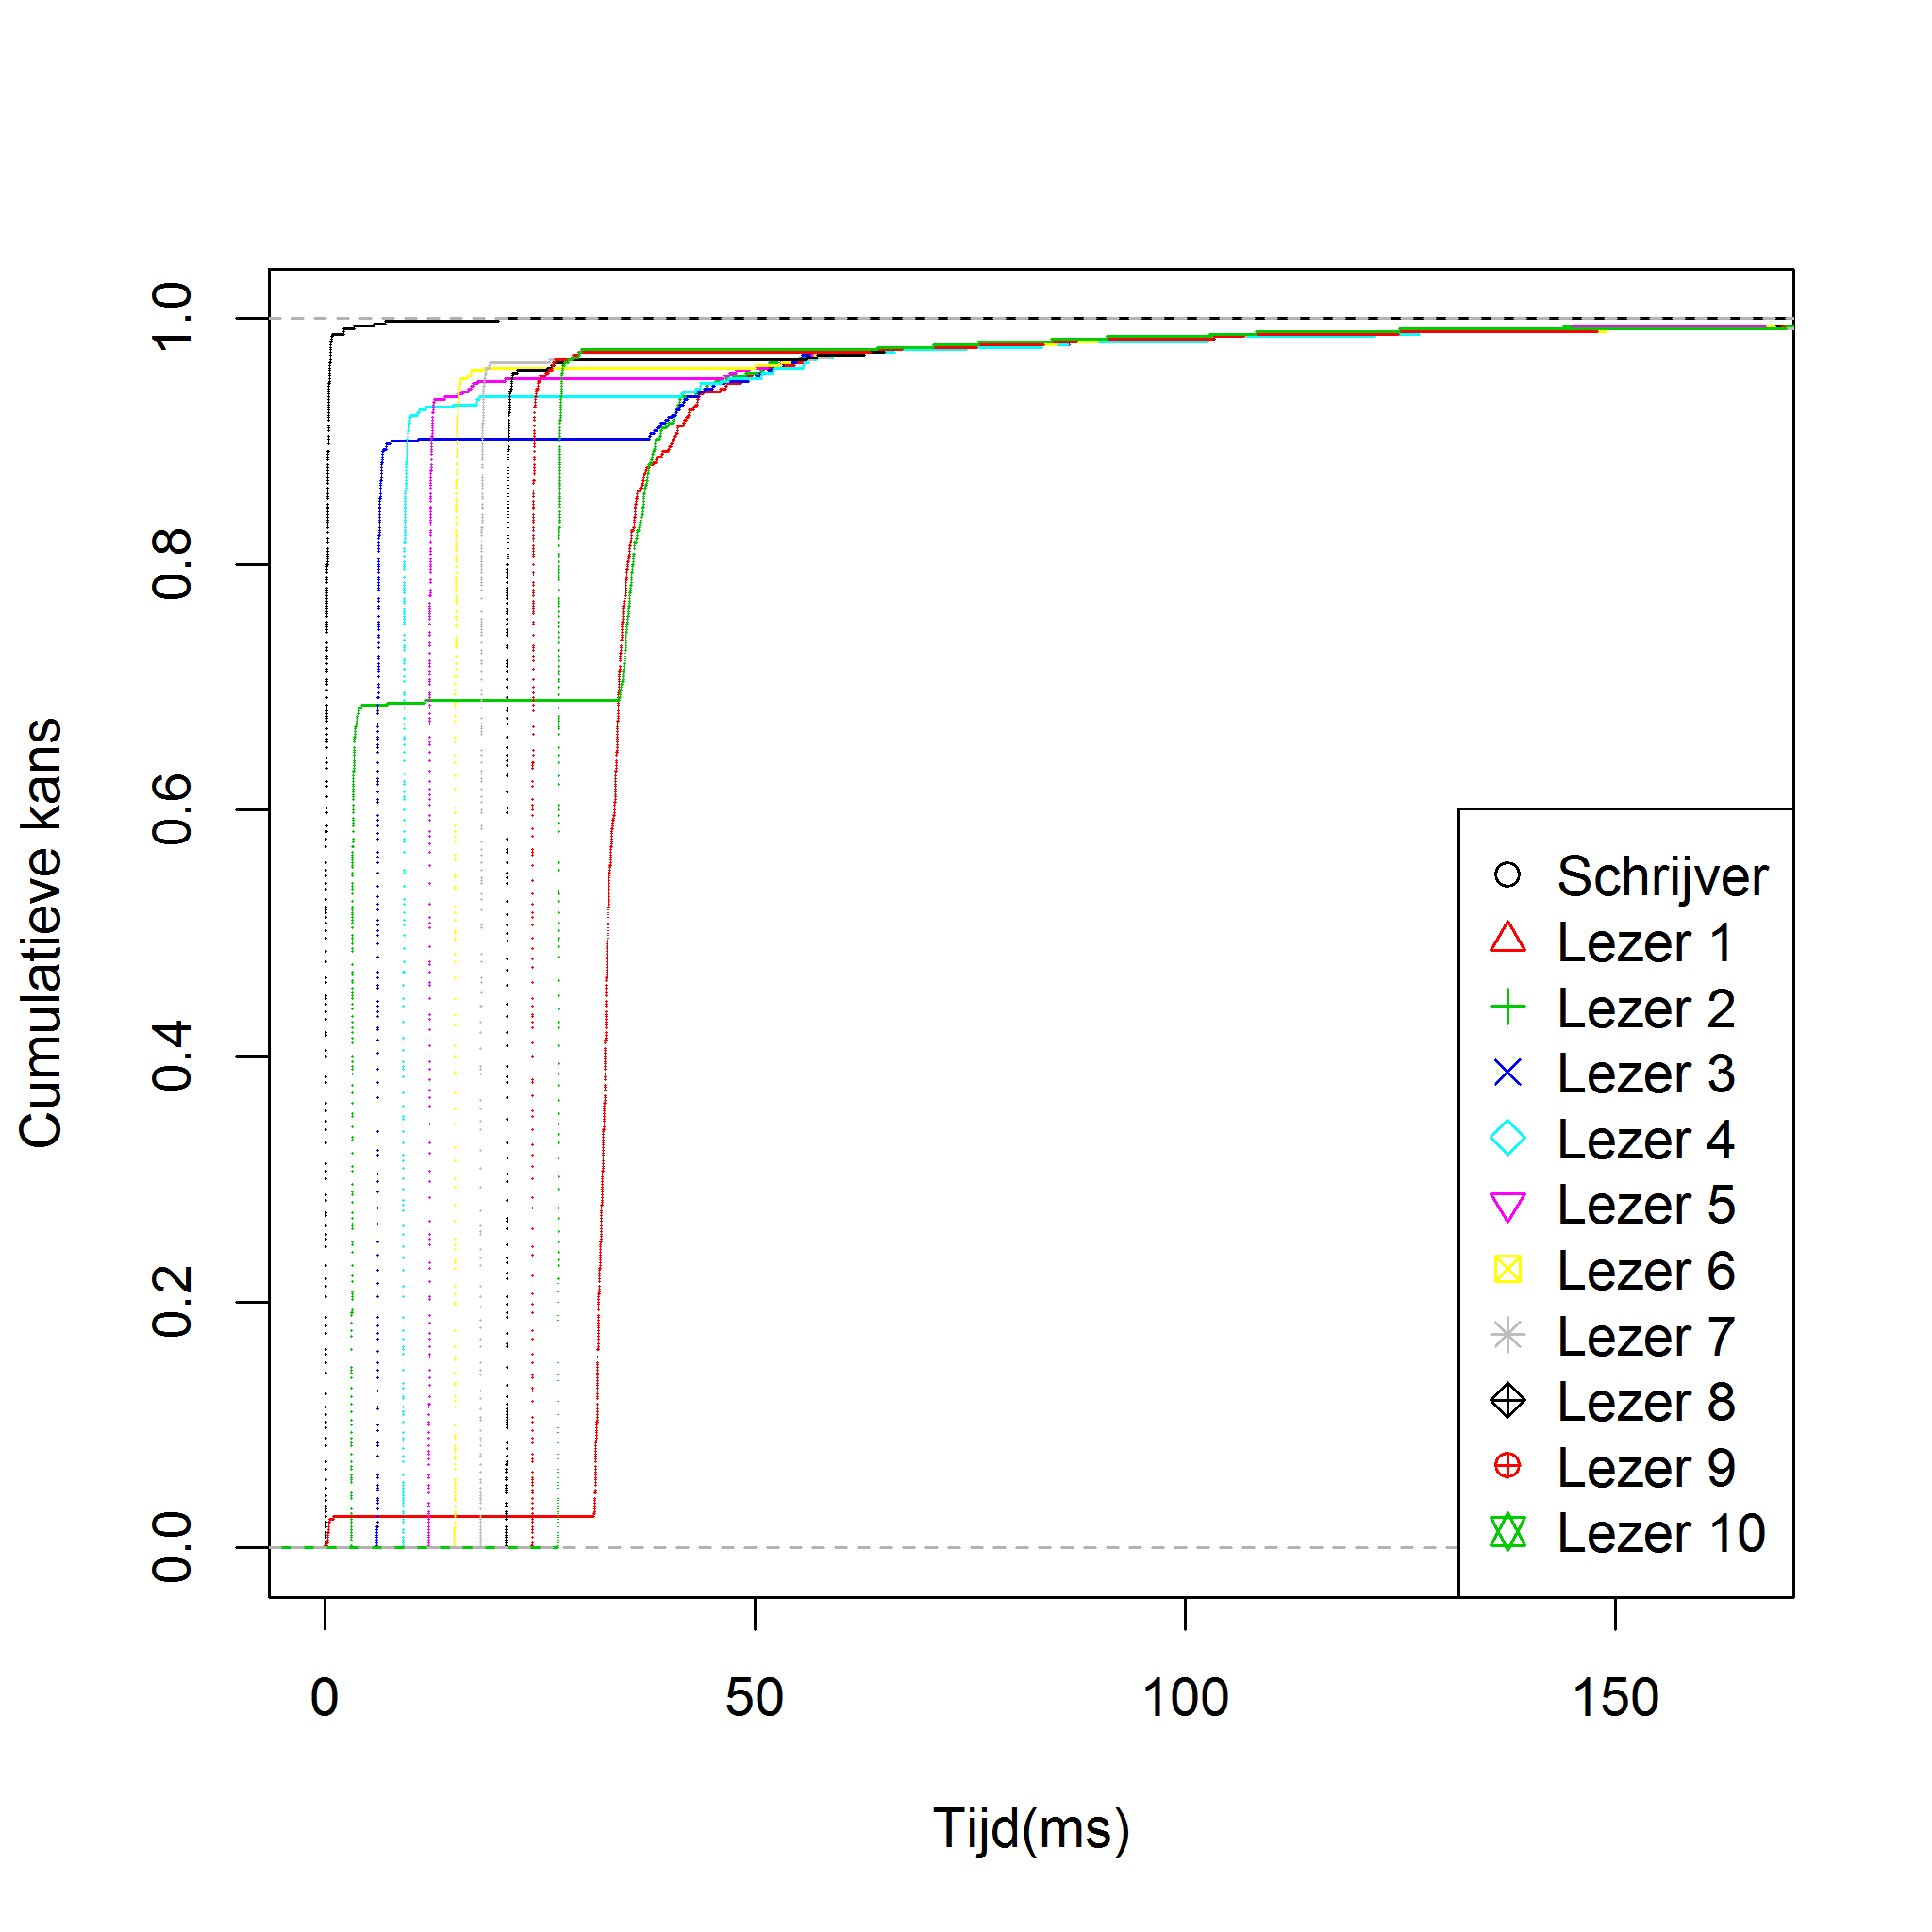
\includegraphics[width=.7\textwidth]{img/Observaties/HBase/ECDF-plot-Start-insertRawData-5}}
	\subfigure{\label{fig:consistentie-hbase-R1} 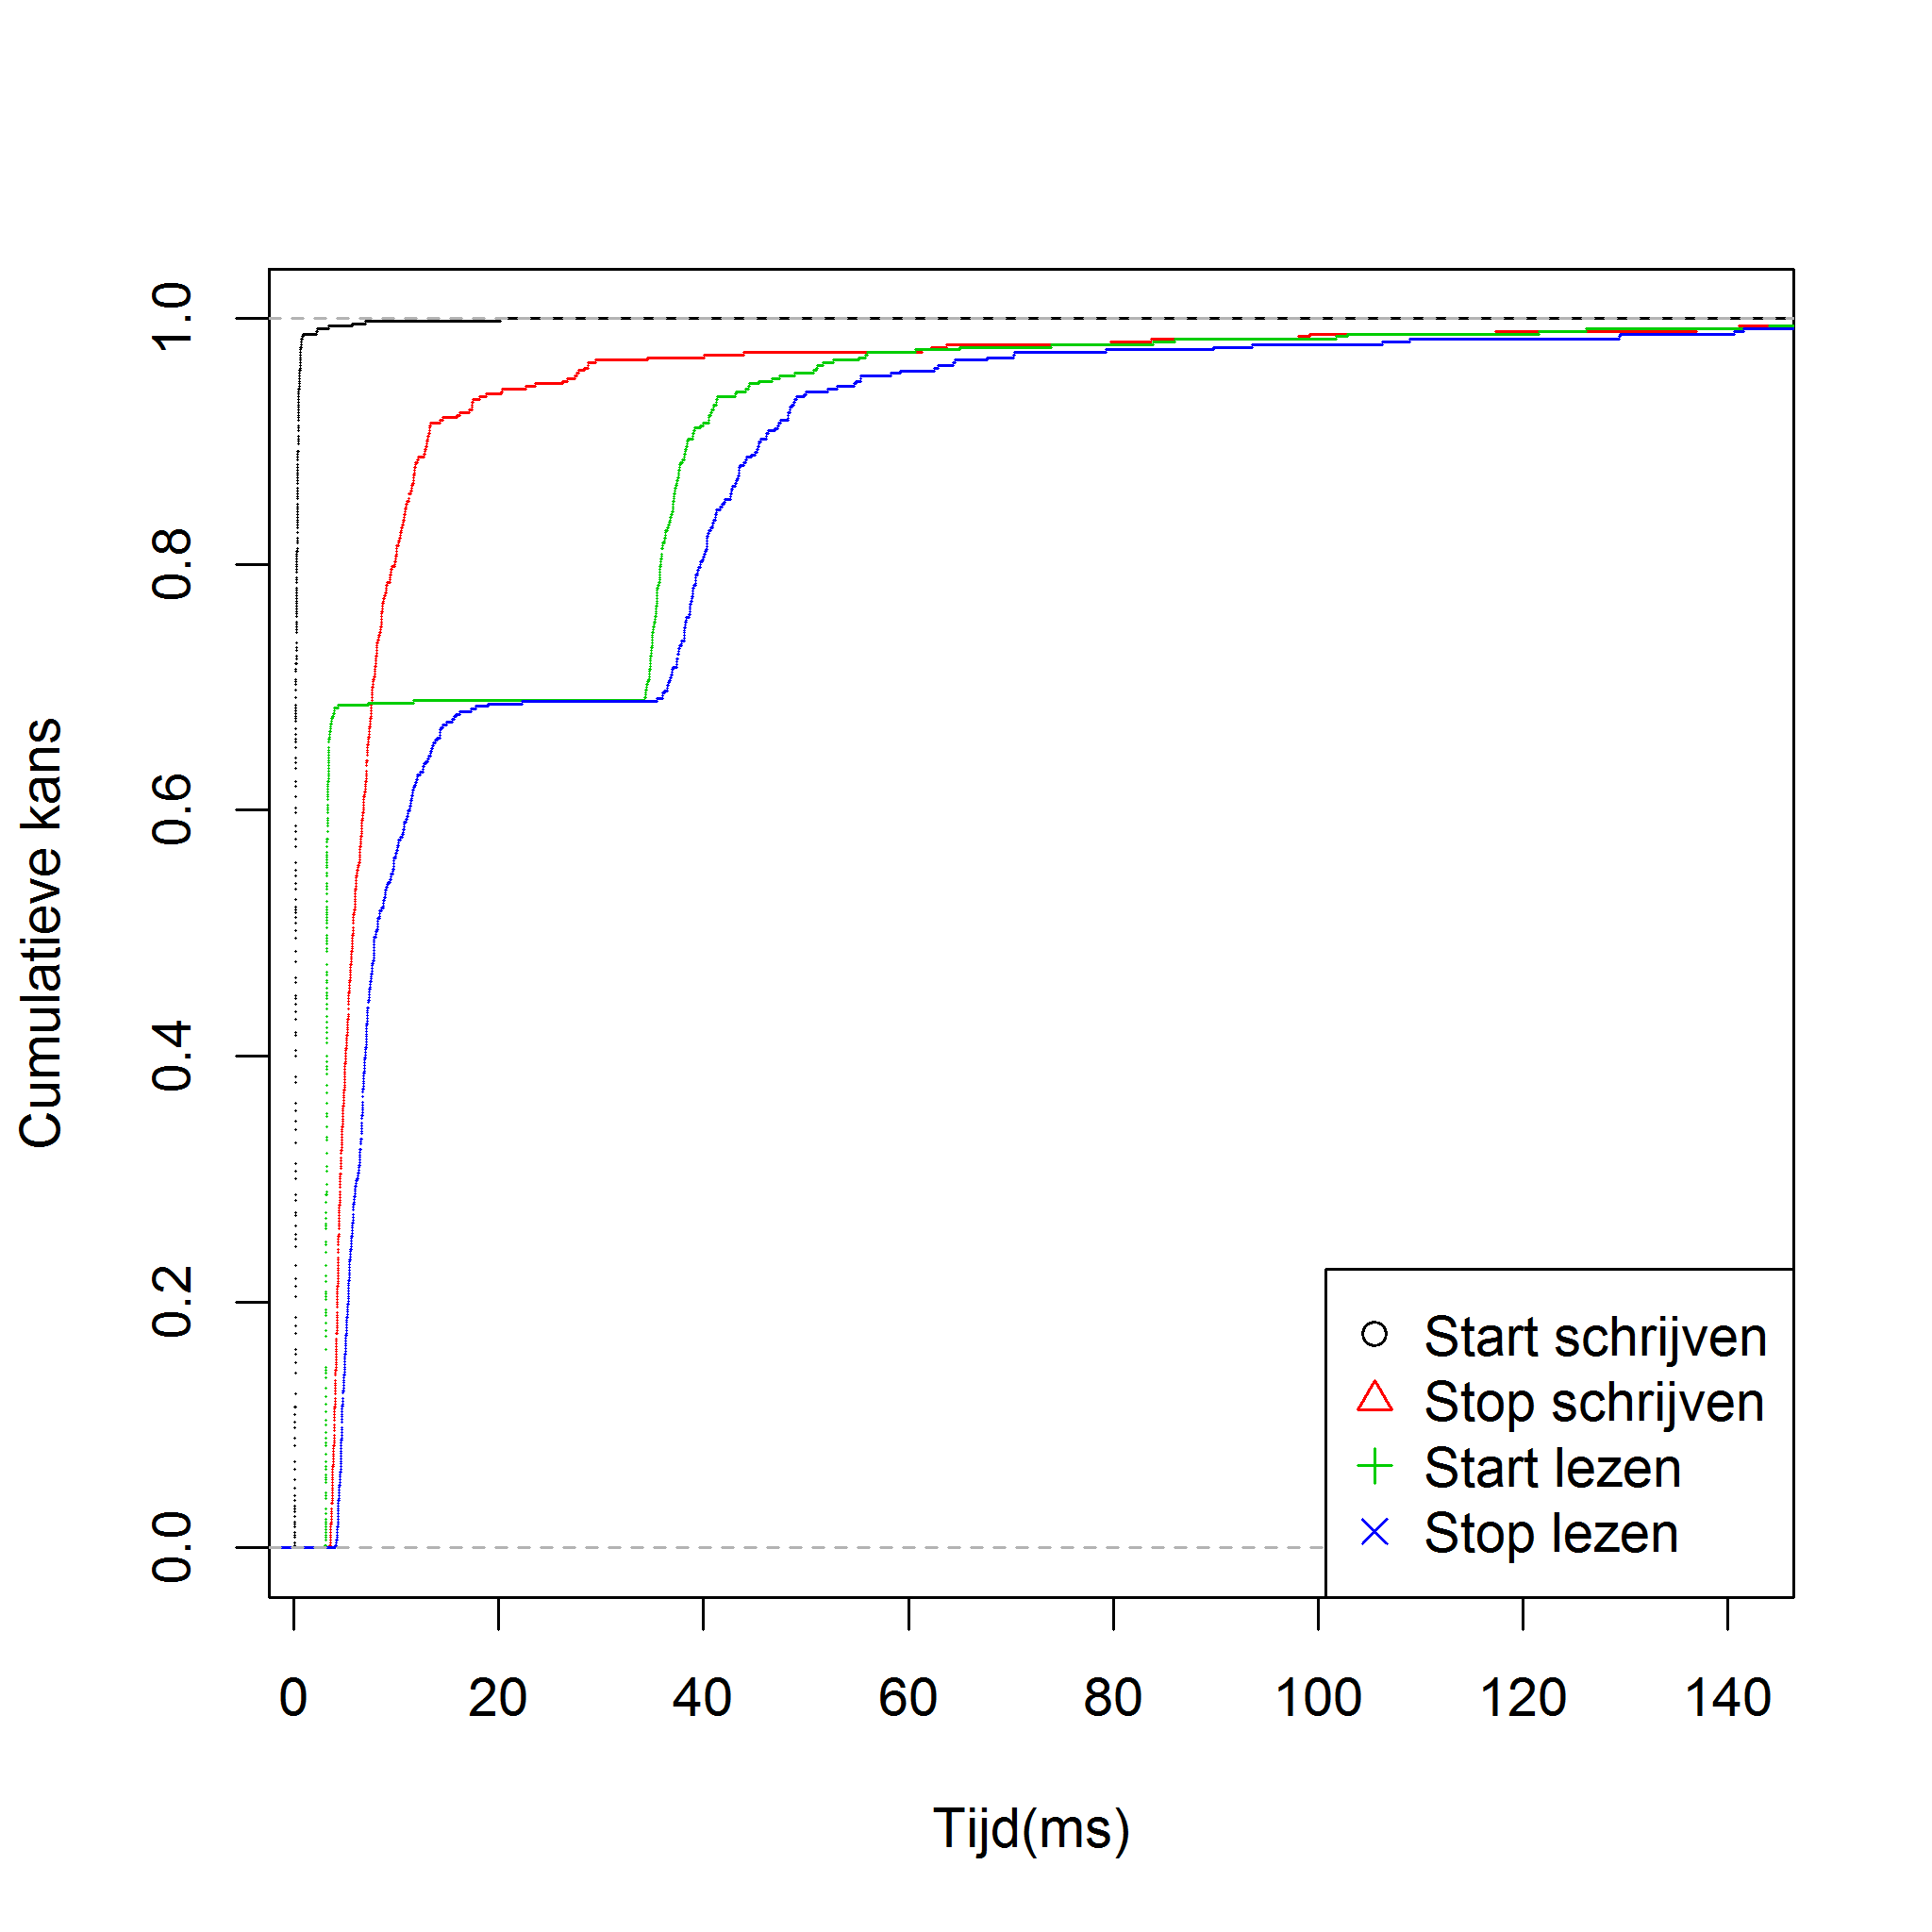
\includegraphics[width=0.7\textwidth]{img/Observaties/HBase/ECDF-plot-R-1-insertRawData-5}}

	\caption{\textbf{Consistentie van HBase} \newline
	HBase heeft geen verschil tussen het invoegen of aanpassen van data naar consistentie, dit zijn dezelfde queries. Daarnaast is de enige configuratie mogelijkheid voor het lezen of schrijven het in- of uitschakelen van de caches aan de gebruikerskant. In al de testen zijn deze uitgeschakeld.  \newline
	Figuur (a) toont een overzicht van de verschillende starttijdstippen voor het lezen van consistente data. Figuur (b) toont de start- en eindtijdstippen voor lezer 2 naast deze voor de schrijver. Lezer 2 start met op 3ms en leest vervolgens elke 30ms tot de nieuwe waarde is gelezen. De maximale waarde van de x-as is zo gekozen dat voor elke dataset minstens 99\% van de data getoond is. }
	\label{fig:consistentie-hbase}
\end{figure}



\begin{figure}[htb!] 
	\centering
	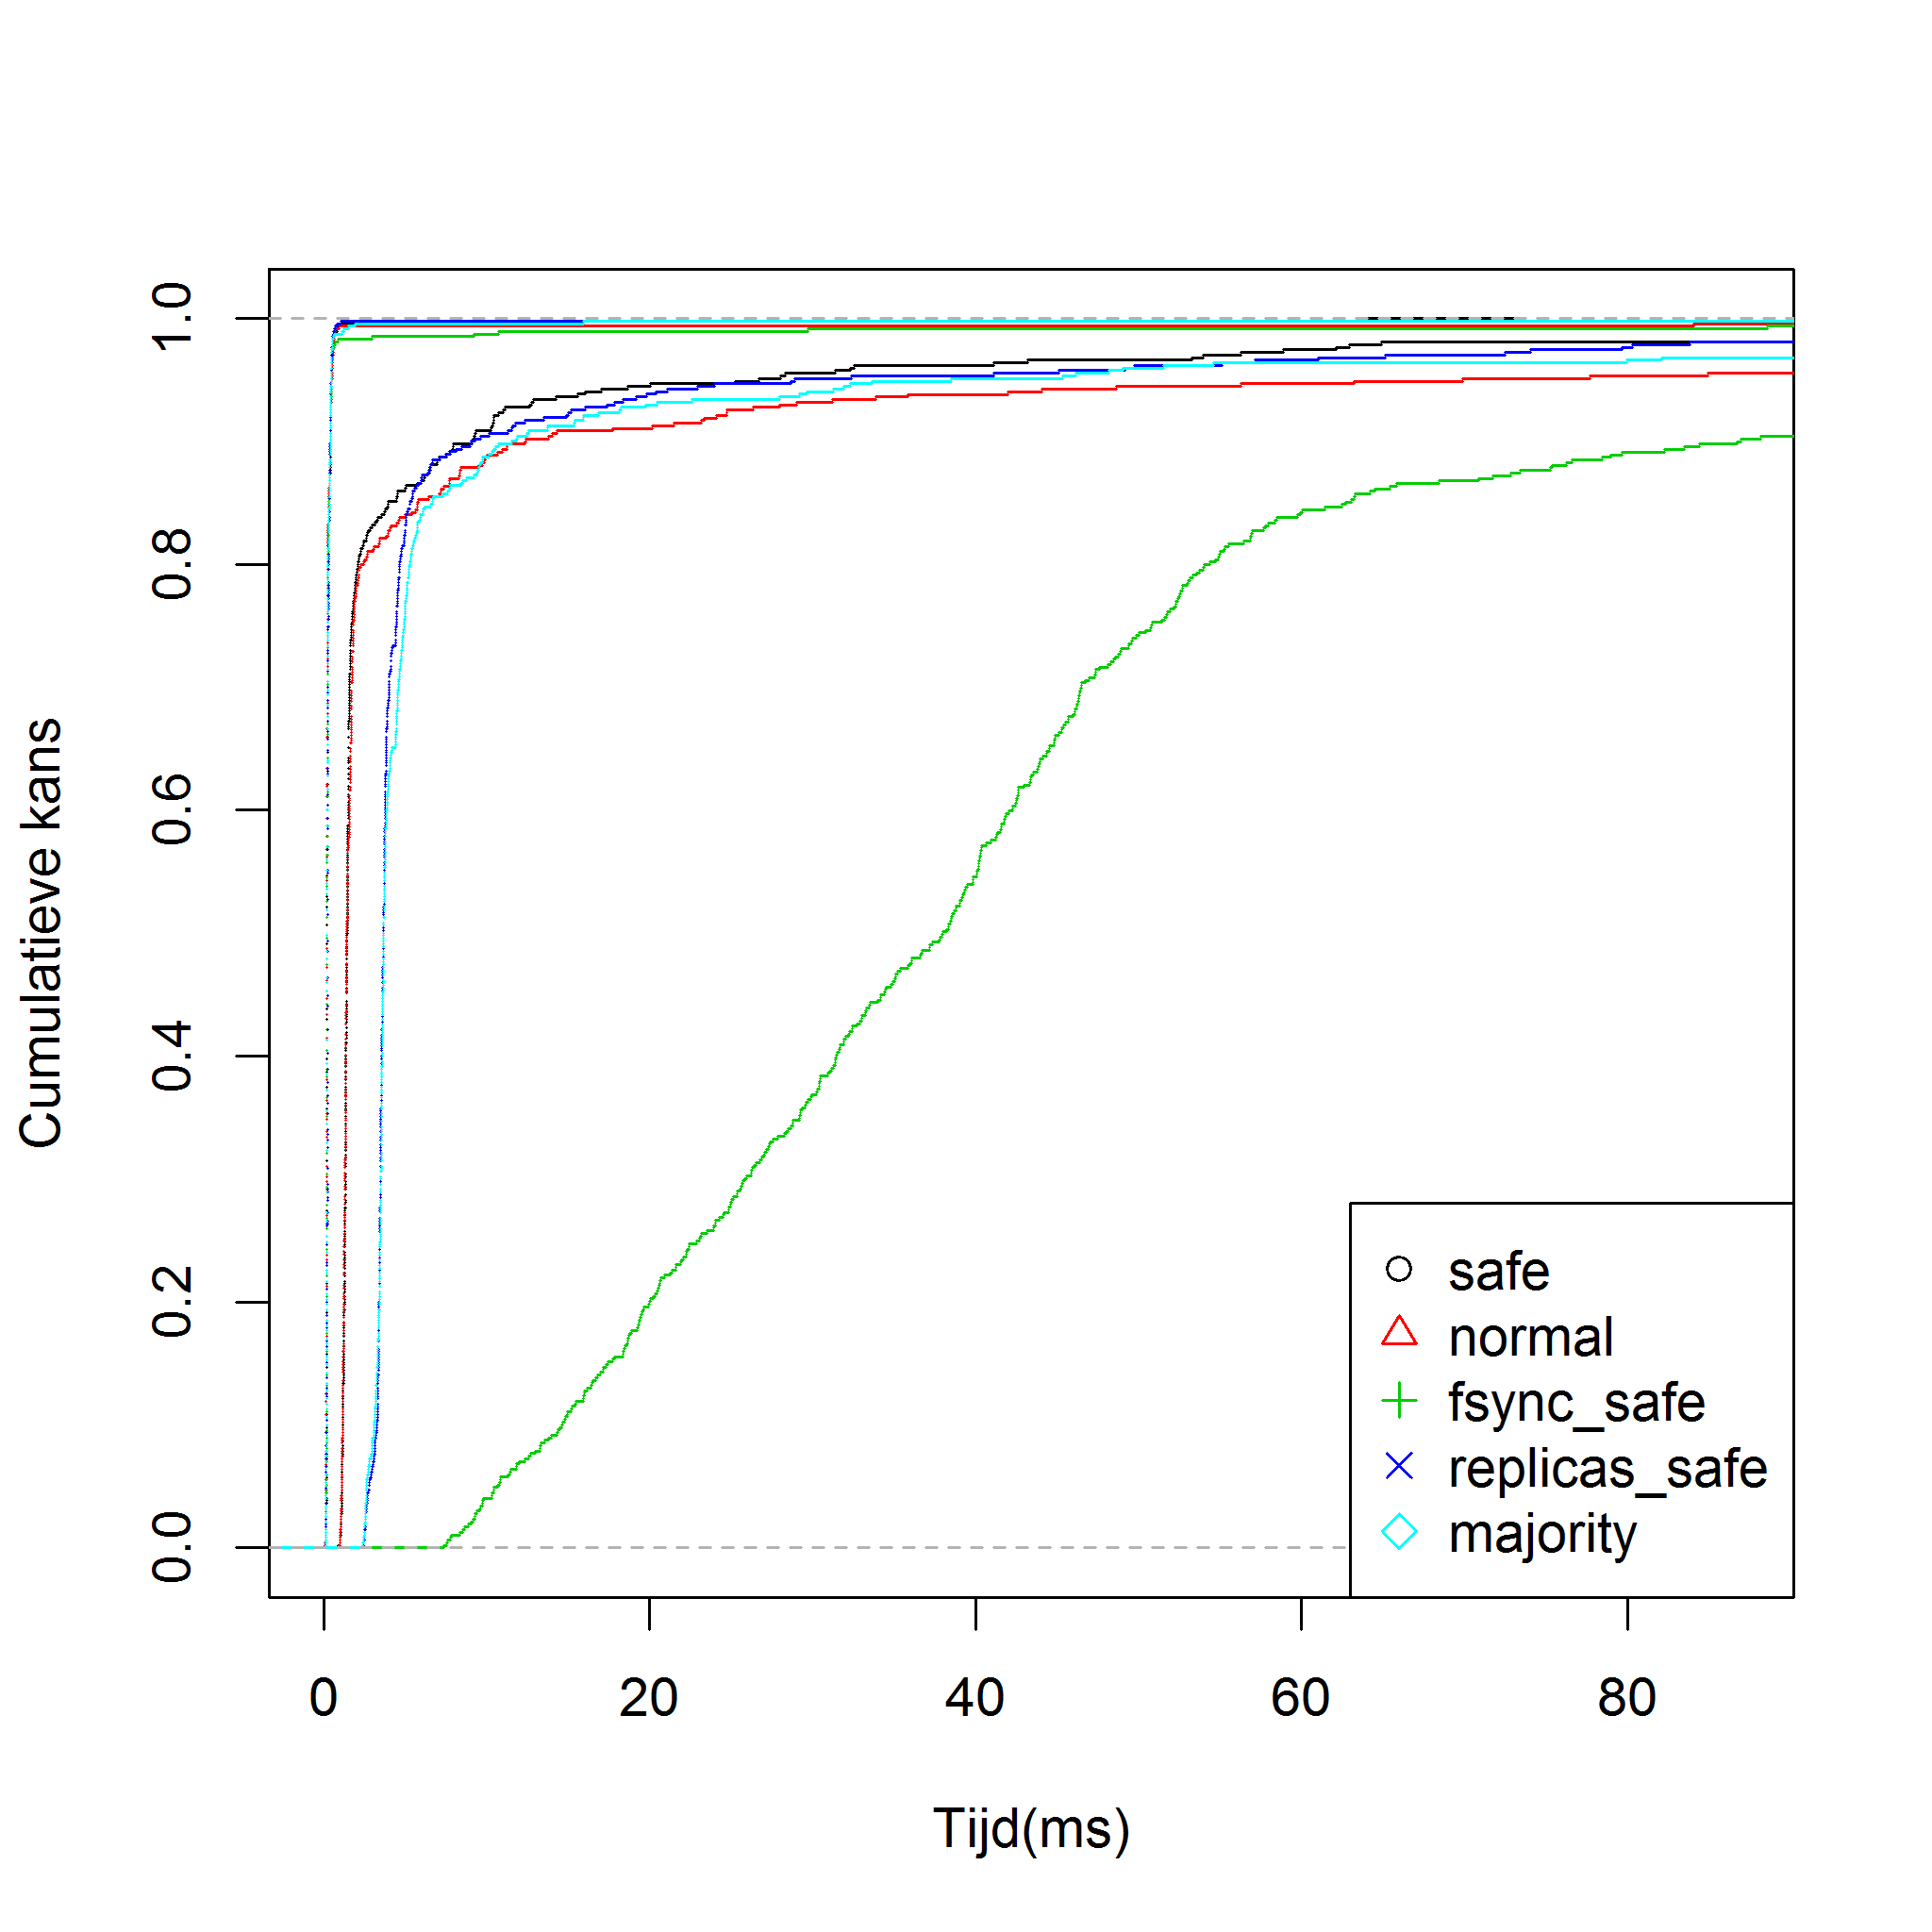
\includegraphics[width=.7\textwidth]{img/Observaties/MongoDB/ECDF-Compare-Write-insert-1}
	\caption{\textbf{Consistentie van MongoDB: Verloop van schrijfoperaties} \newline
	Dit is de ruwe data van MongoDB's verschillende schrijfoperaties met een 90-percentiel, de start- en stoptijden zijn in dezelfde kleur.  }
	\label{fig:consistentie-mongodb-all-mongodb-write}
\end{figure}

\begin{figure}[ht!] 
	\centering 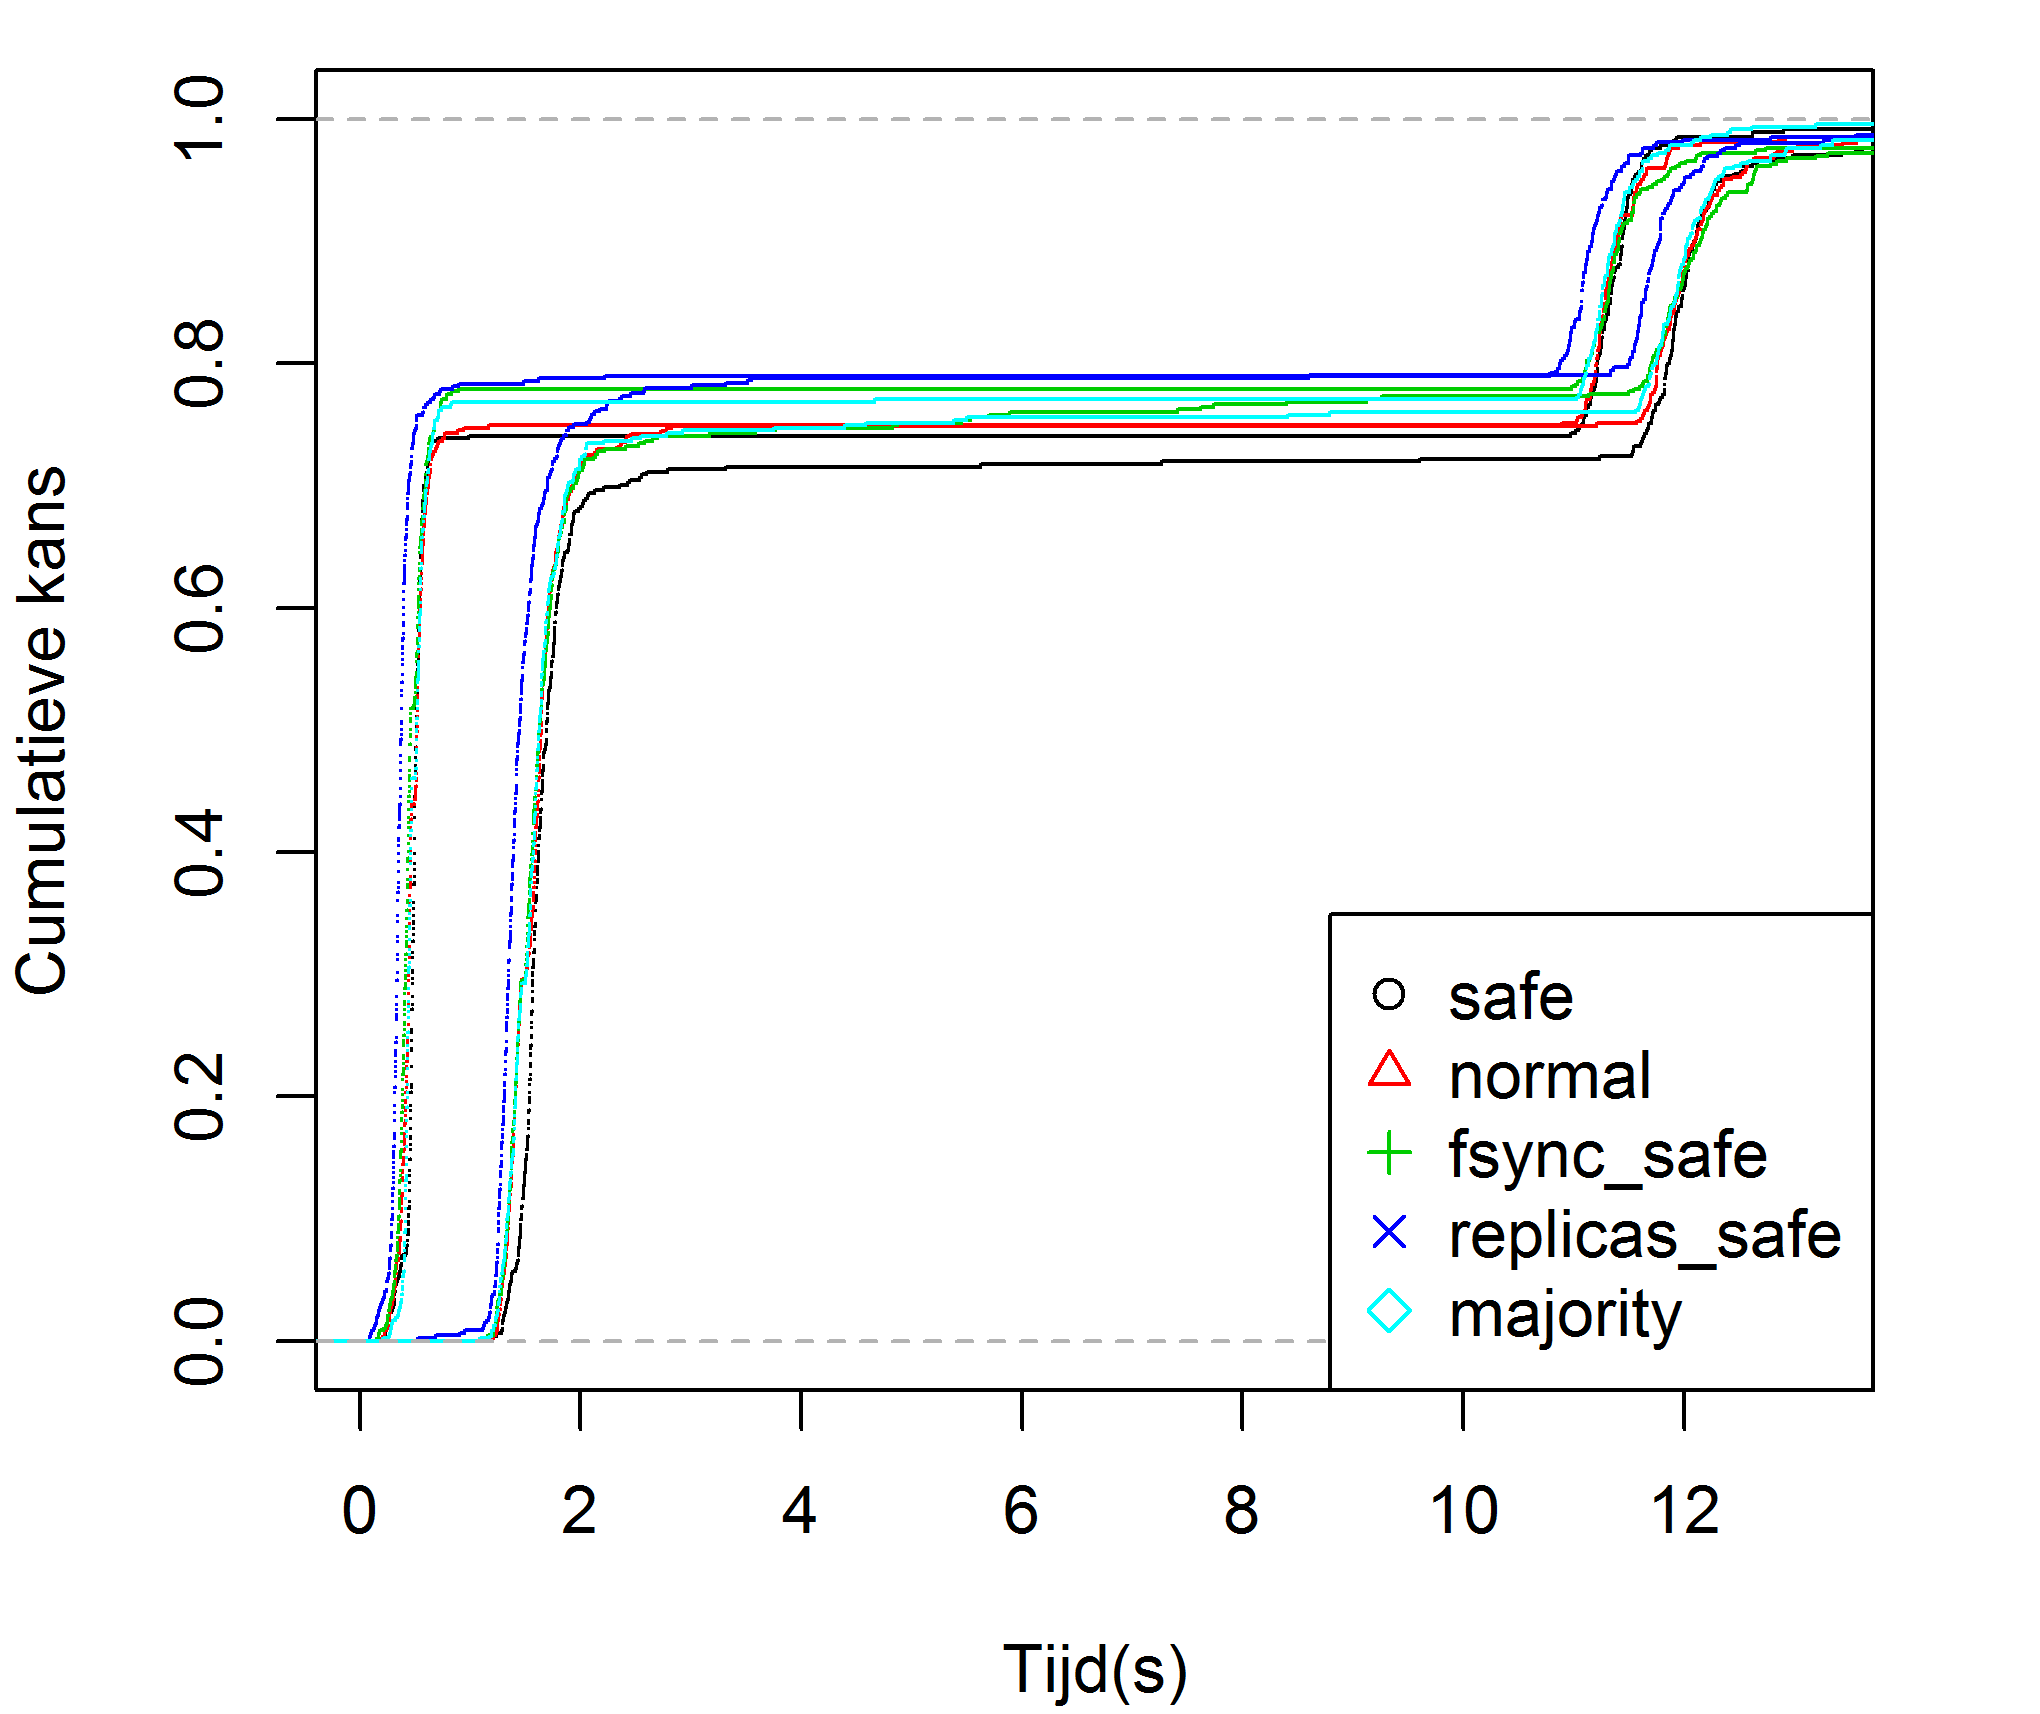
\includegraphics[width=.70\textwidth]{img/Observaties/MongoDB/ECDF-Write-update-primarypreferred-1-2}
	\caption{\textbf{Consistentie van MongoDB: Leesgedrag bij verschillende schrijfconfiguraties } \newline
	Een vergelijking van het leesgedrag onder verschillende schrijfconfiguratie toont dat er geen significant verschil is. In de figuur is een 99-percentiel getoond voor een update operatie met als leesactie primary, de start- en stoptijden zijn in dezelfde kleur.  
	 } 
	\label{fig:consistentie-mongodb-verschillende-schrijfacties}
\end{figure}

\begin{figure}[ht!] 
	\centering
	\subfigure[Majority Update]{\label{fig:consistentie-mongodb-R2-majority} 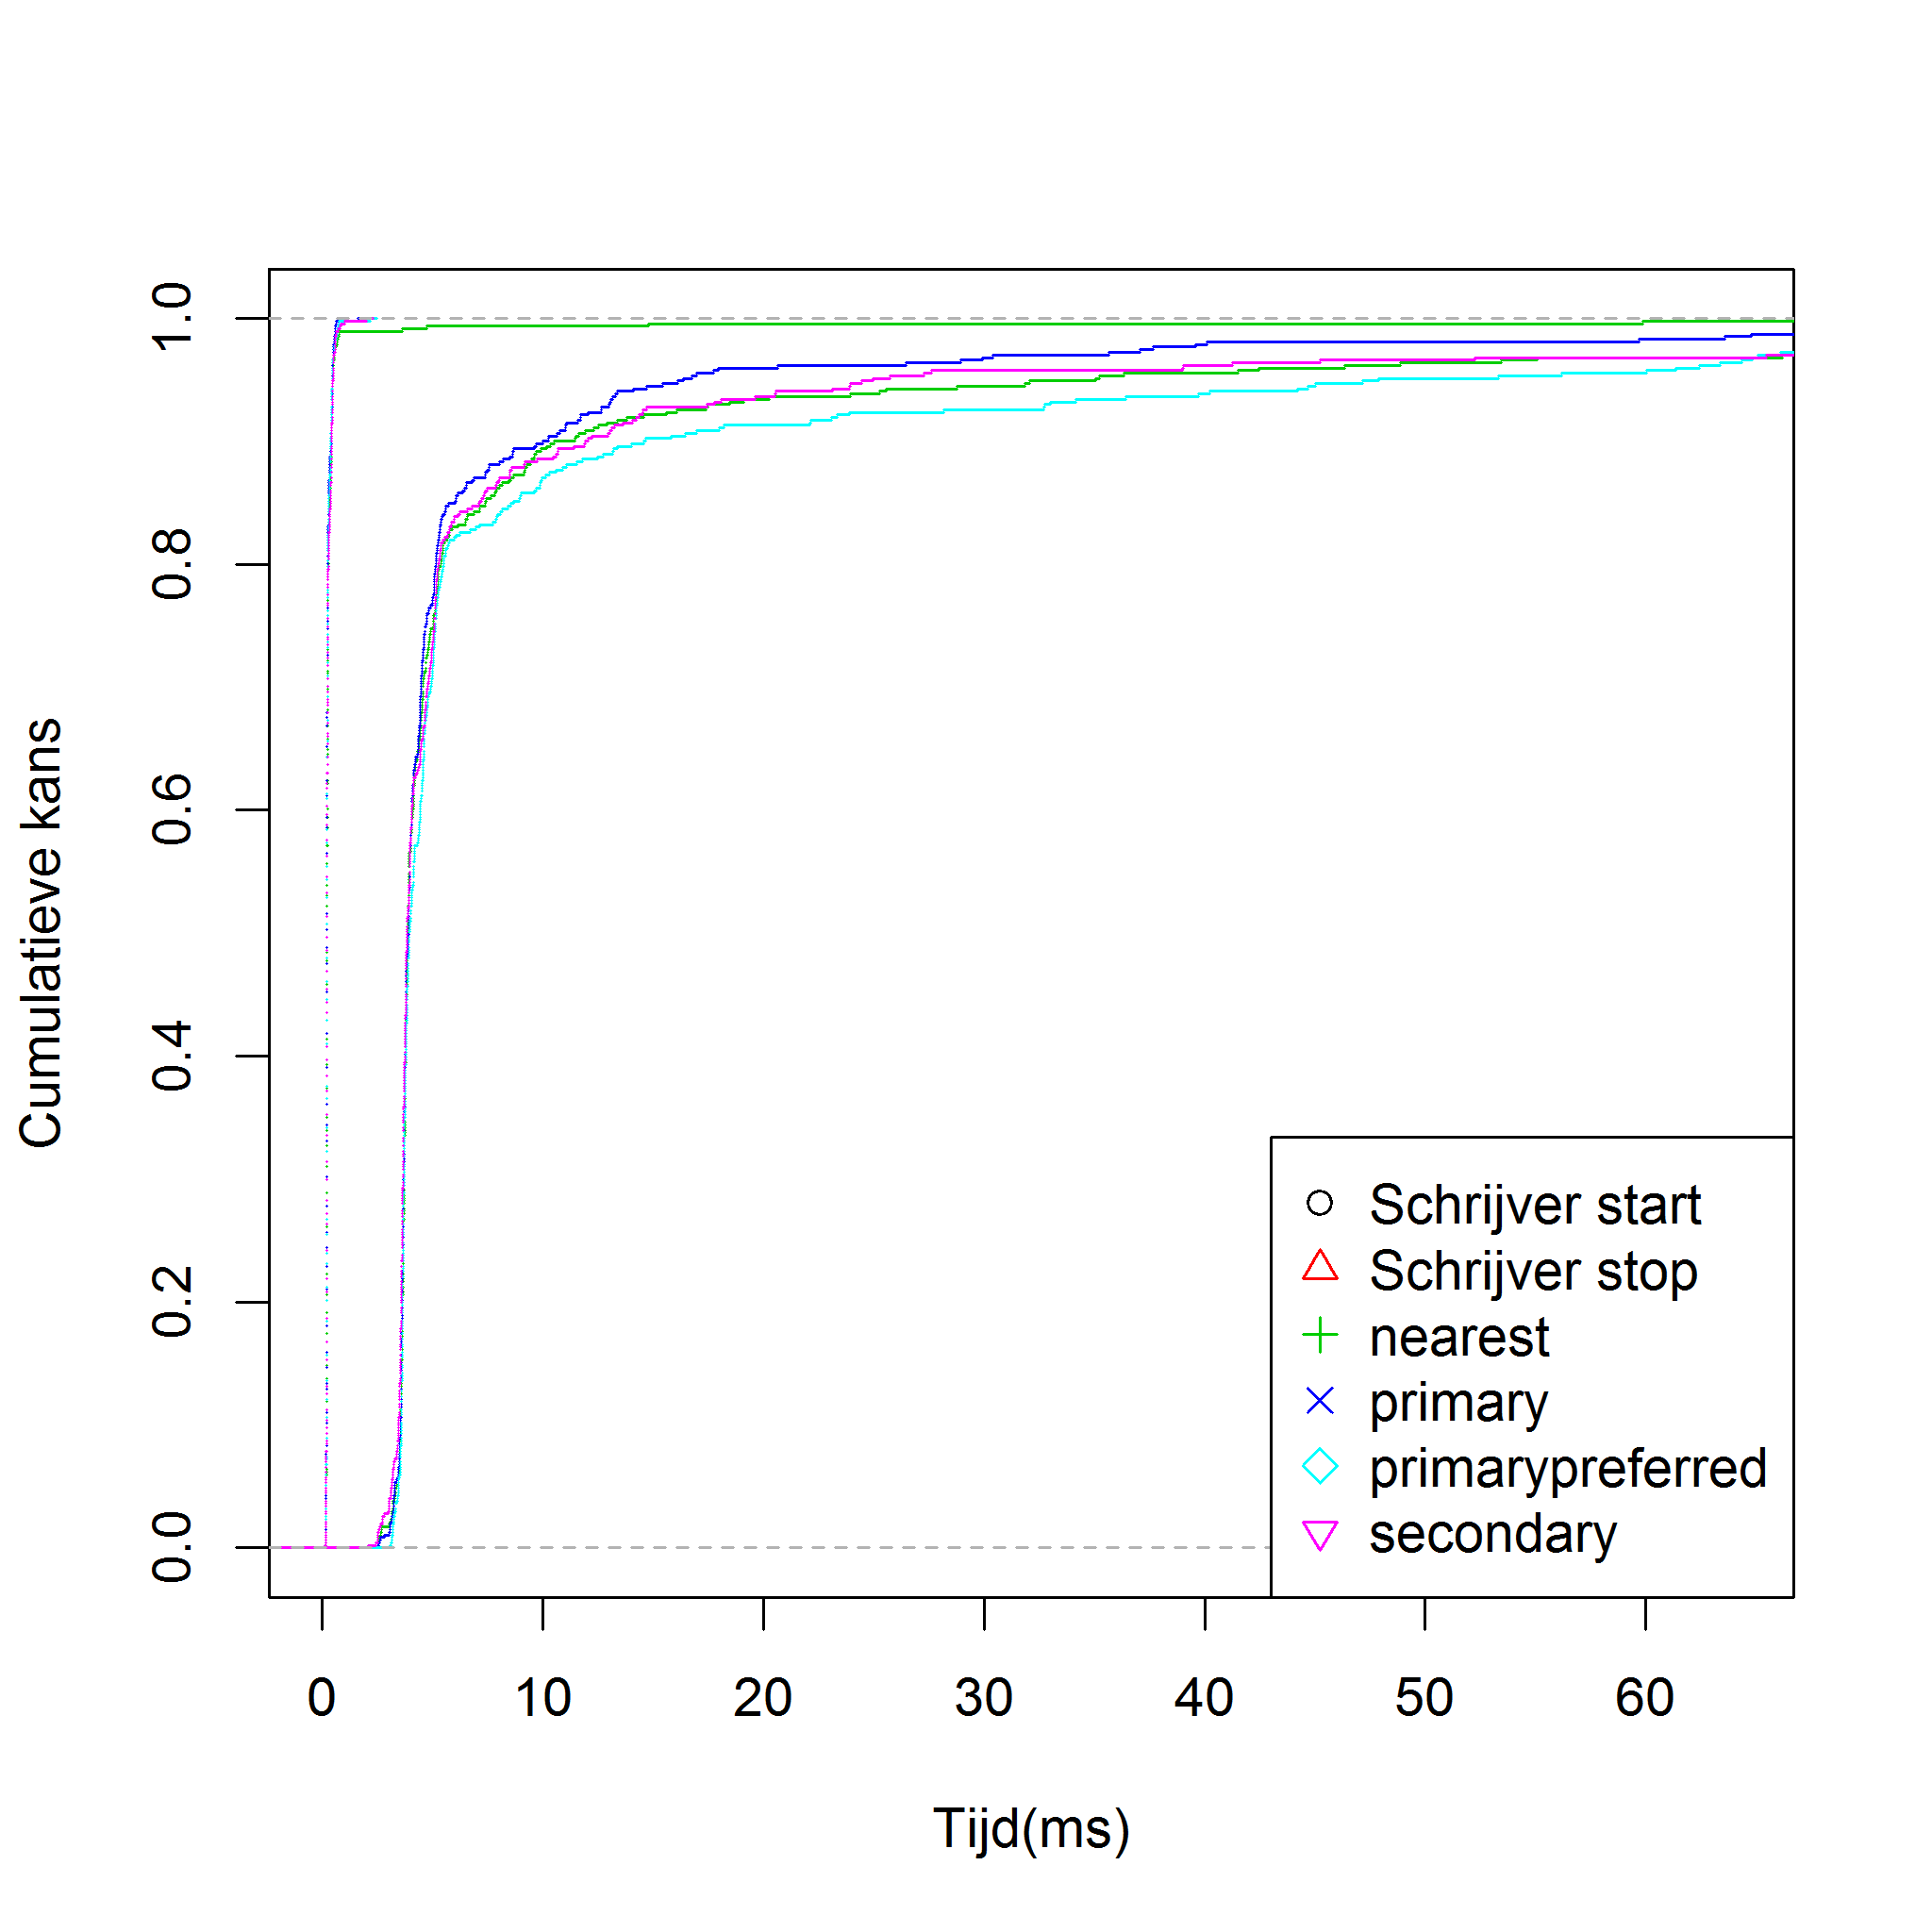
\includegraphics[width=.70\textwidth]{img/Observaties/MongoDB/ECDF-Reads-update-majority-1-2}}
	\subfigure[Majority Insert]{\label{fig:consistentie-mongodb-R2-majority-insert} 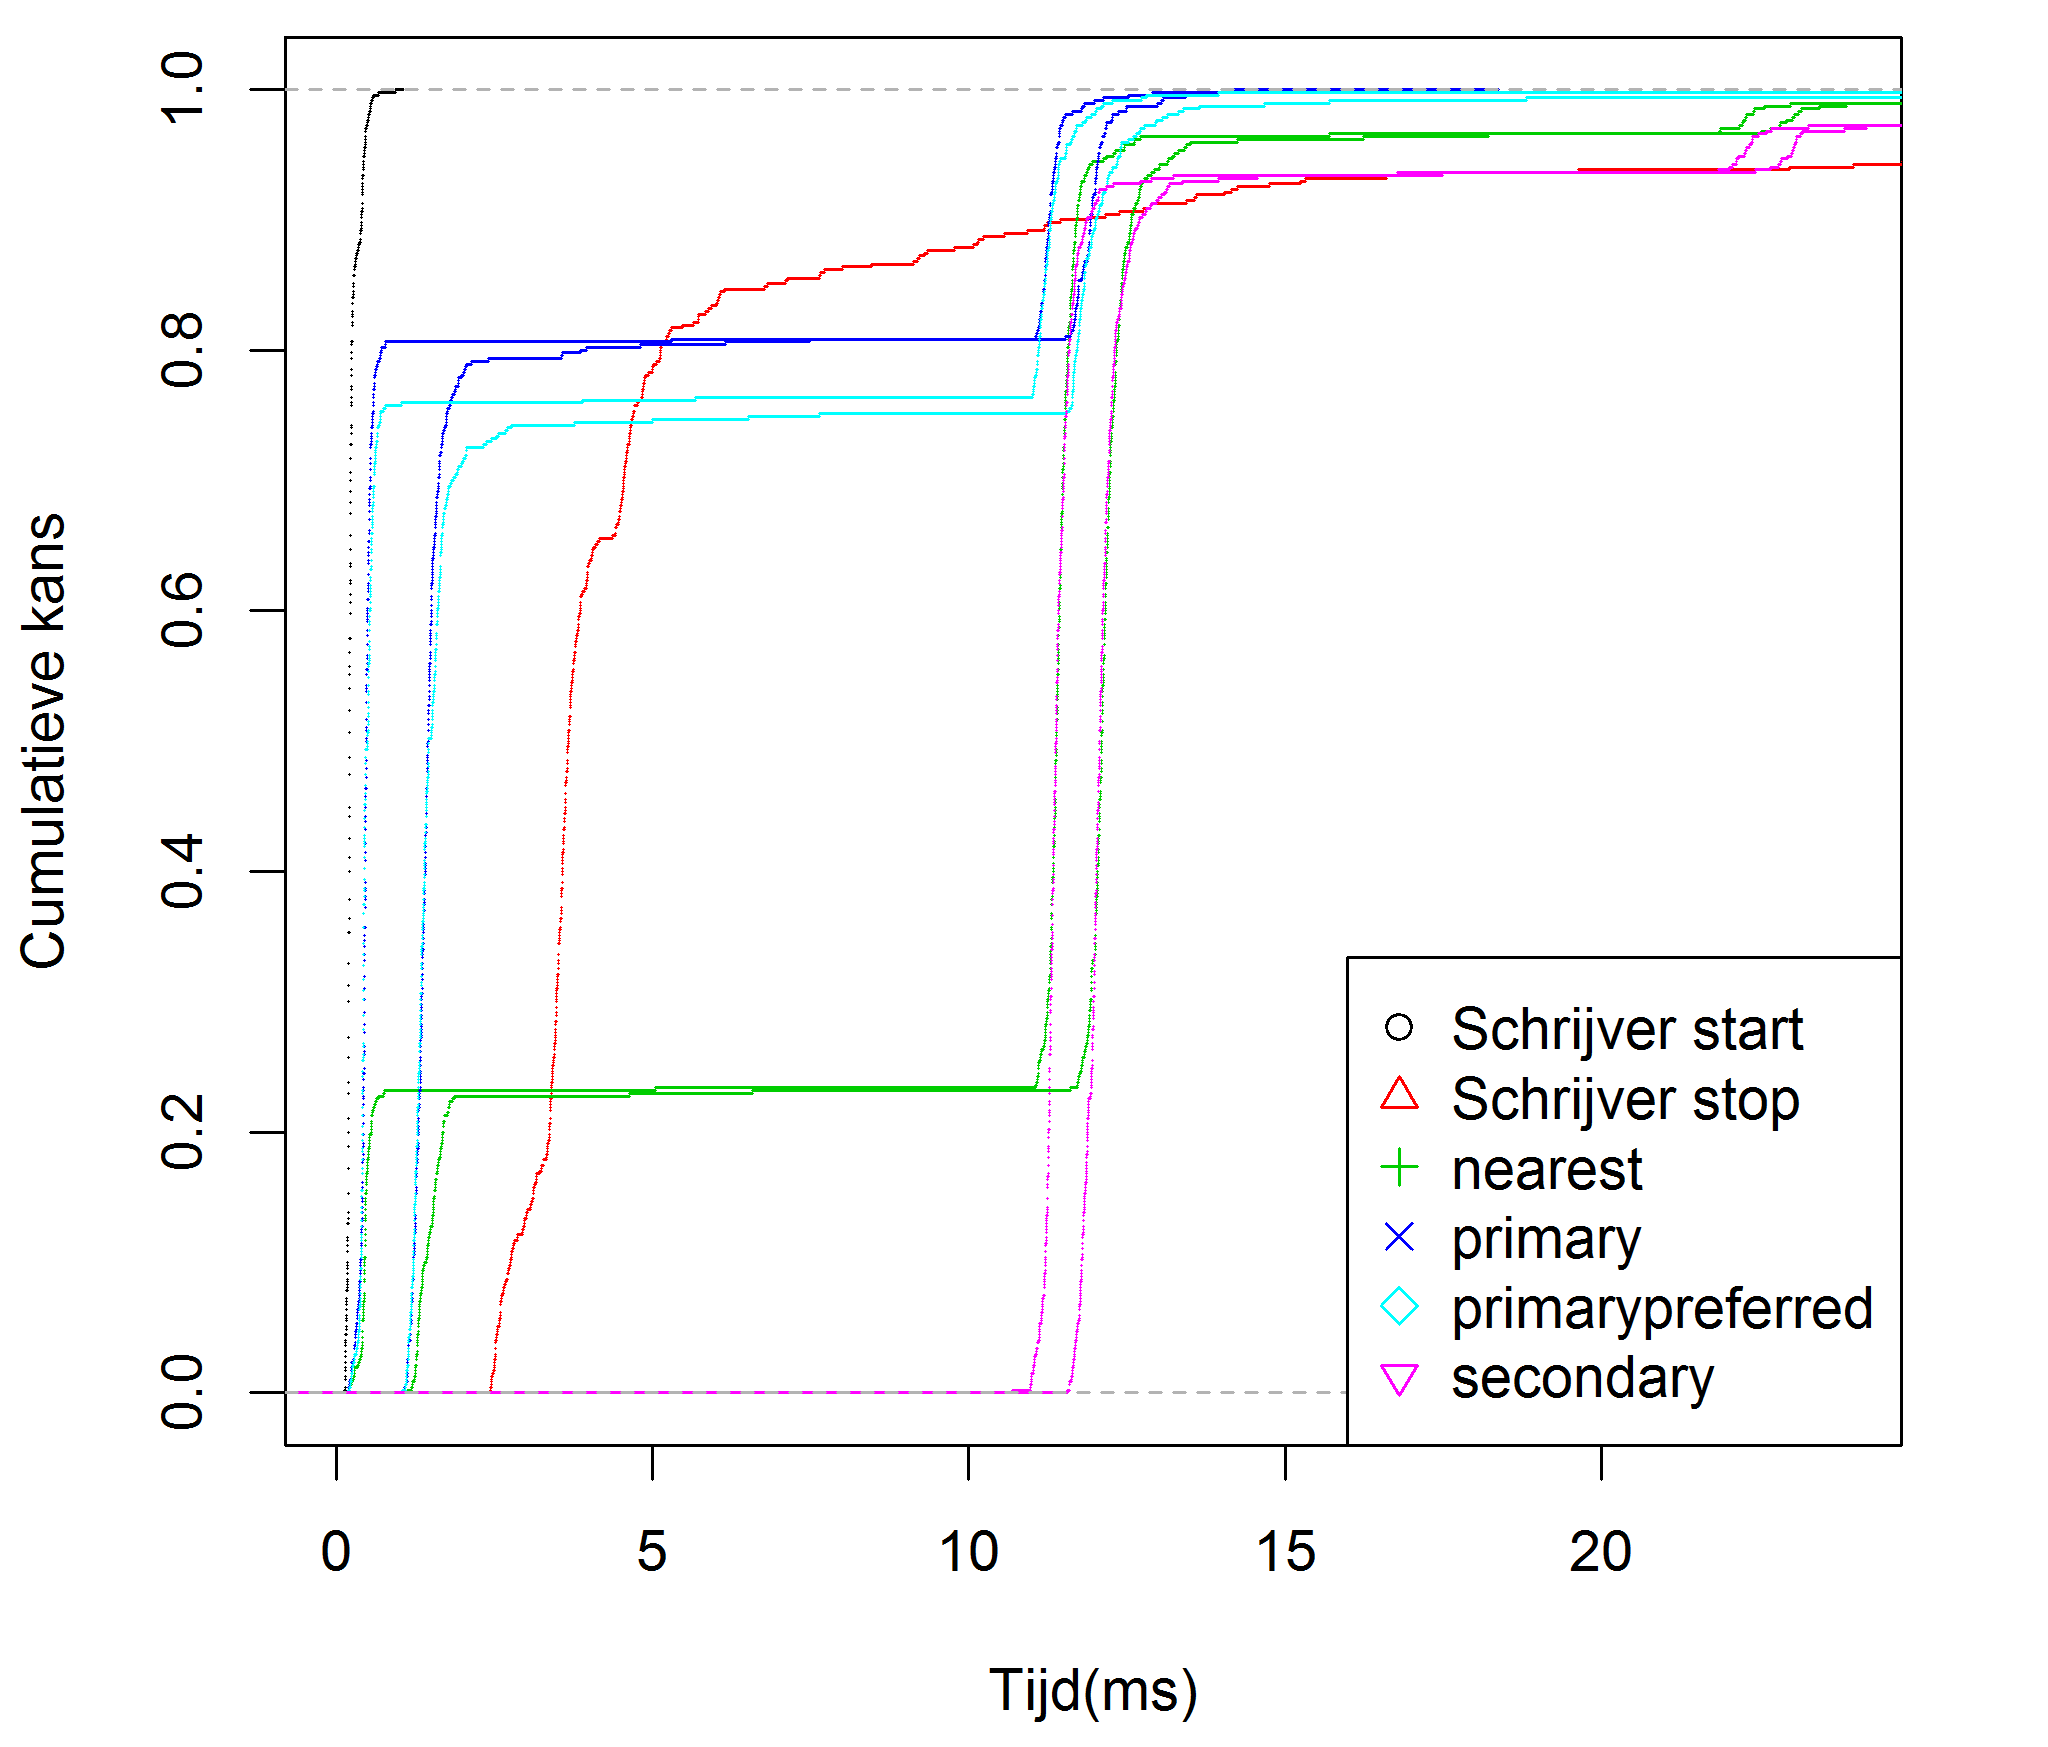
\includegraphics[width=.70\textwidth]{img/Observaties/MongoDB/ECDF-Reads-insert-majority-1-2}}
	\caption{\textbf{Consistentie van MongoDB: Insert vs Update voor lezer 2} \newline
	Overzicht van MongoDB's insert vs update met een 99-percentiel voor lezer 2. De start- en stoptijden zijn in dezelfde kleur. Lezer 2 start met lezen op 2ms en vervolgens elke 10ms. Er is geen significant verschil tussen een insert of een update bij dezelfde leesconfiguratie en dezelfde lezer.  }
	\label{fig:consistentie-mongodb-update-vs-insert}
\end{figure}


\begin{figure}[ht!] 
	\centering
	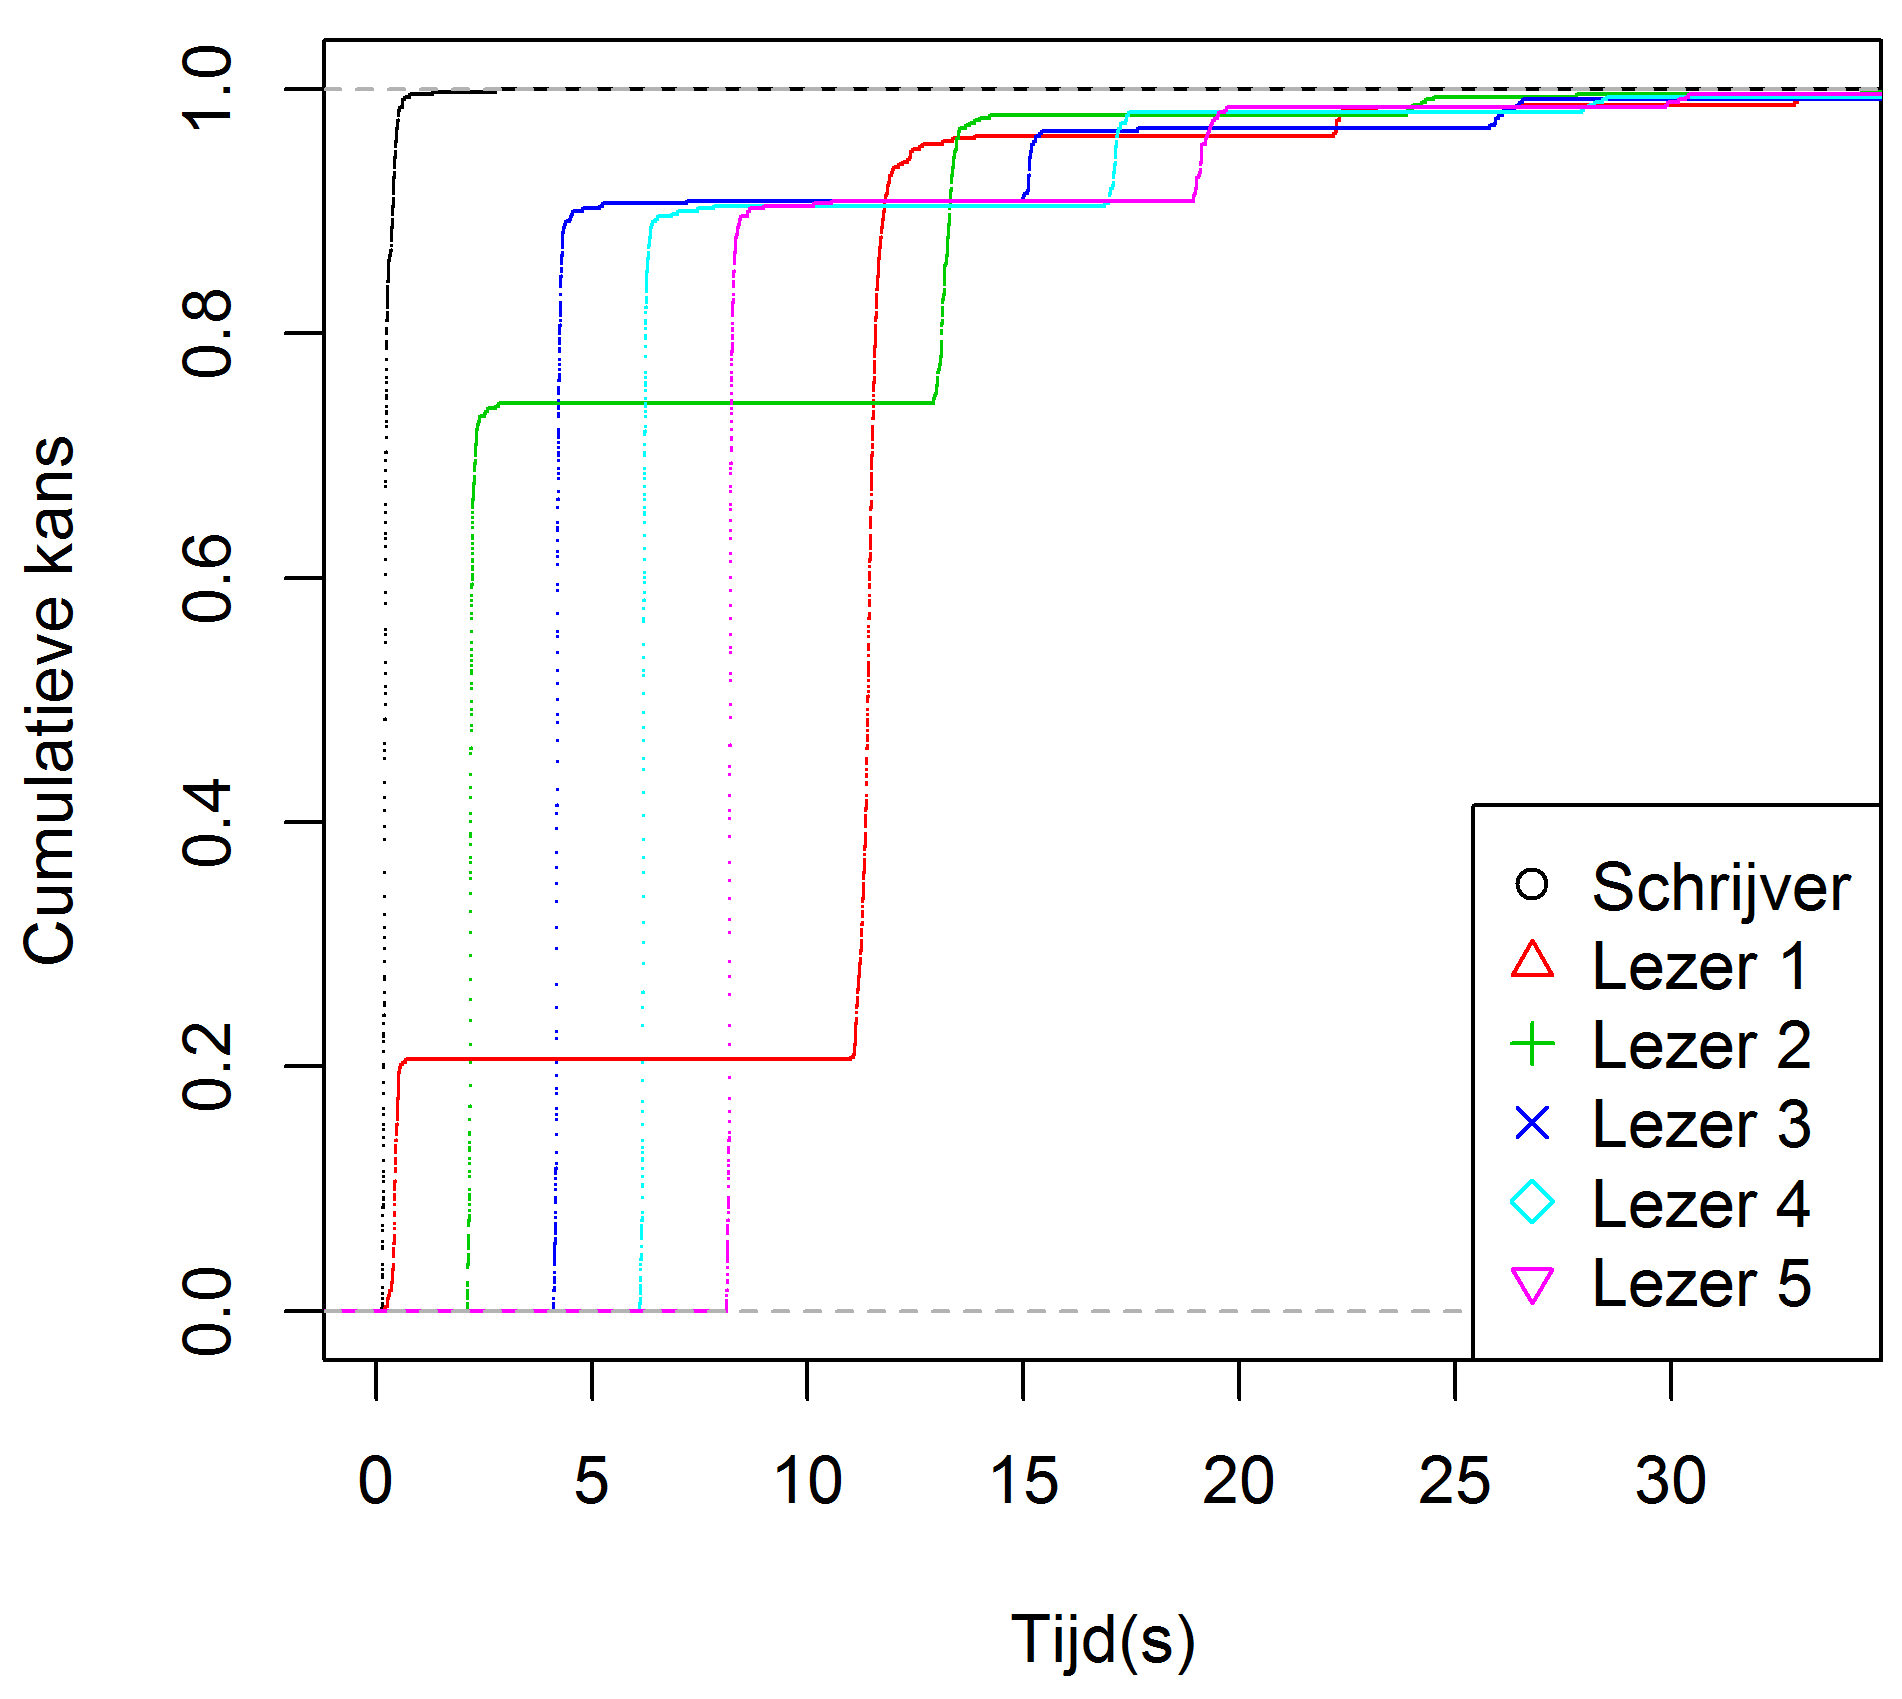
\includegraphics[width=.70\textwidth]{img/Observaties/MongoDB/ECDF-plot-Start-updateRawData-majority-nearest-1}
	\caption{\textbf{Consistentie van MongoDB}: Overzicht van startmoment van consistente leesactie voor het lezen op de nearest }
	\label{fig:consistentie-mongodb-nearest}
\end{figure}
\begin{figure}[htb!] 
	\centering
	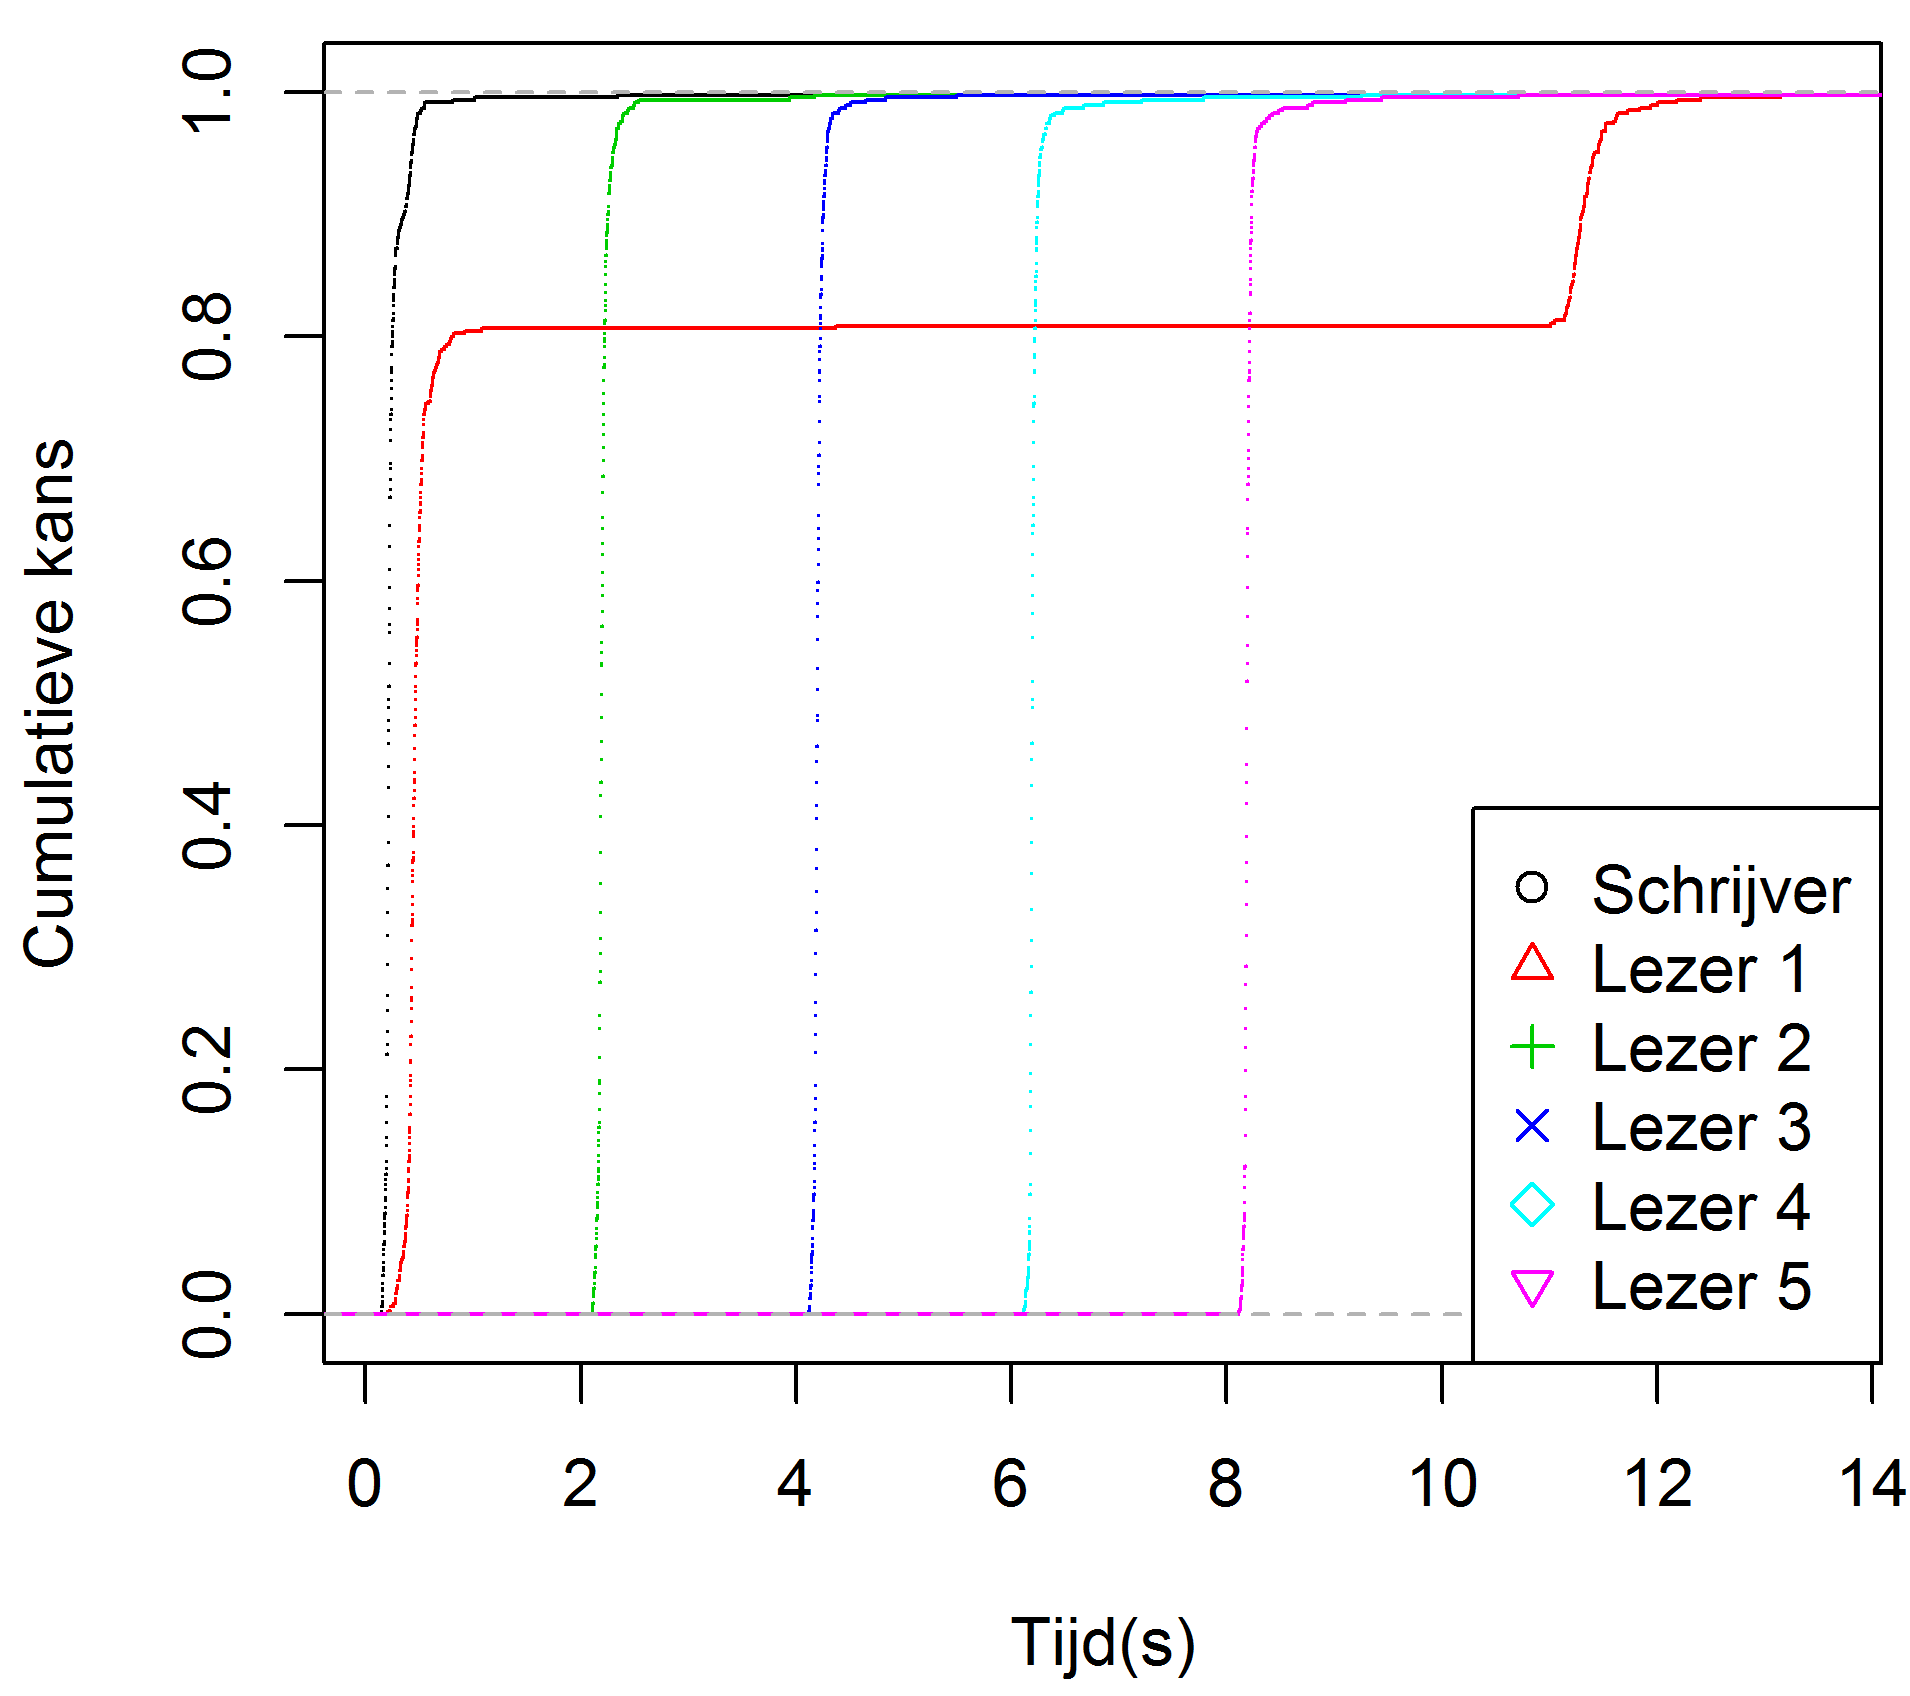
\includegraphics[width=.70\textwidth]{img/Observaties/MongoDB/ECDF-plot-Start-updateRawData-majority-primary-1}
	\caption{\textbf{Consistentie van MongoDB}: Overzicht van startmoment van consistente leesactie voor het lezen op de primary }
	\label{fig:consistentie-mongodb-primary}
\end{figure}
\begin{figure}[htb!] 
	\centering
	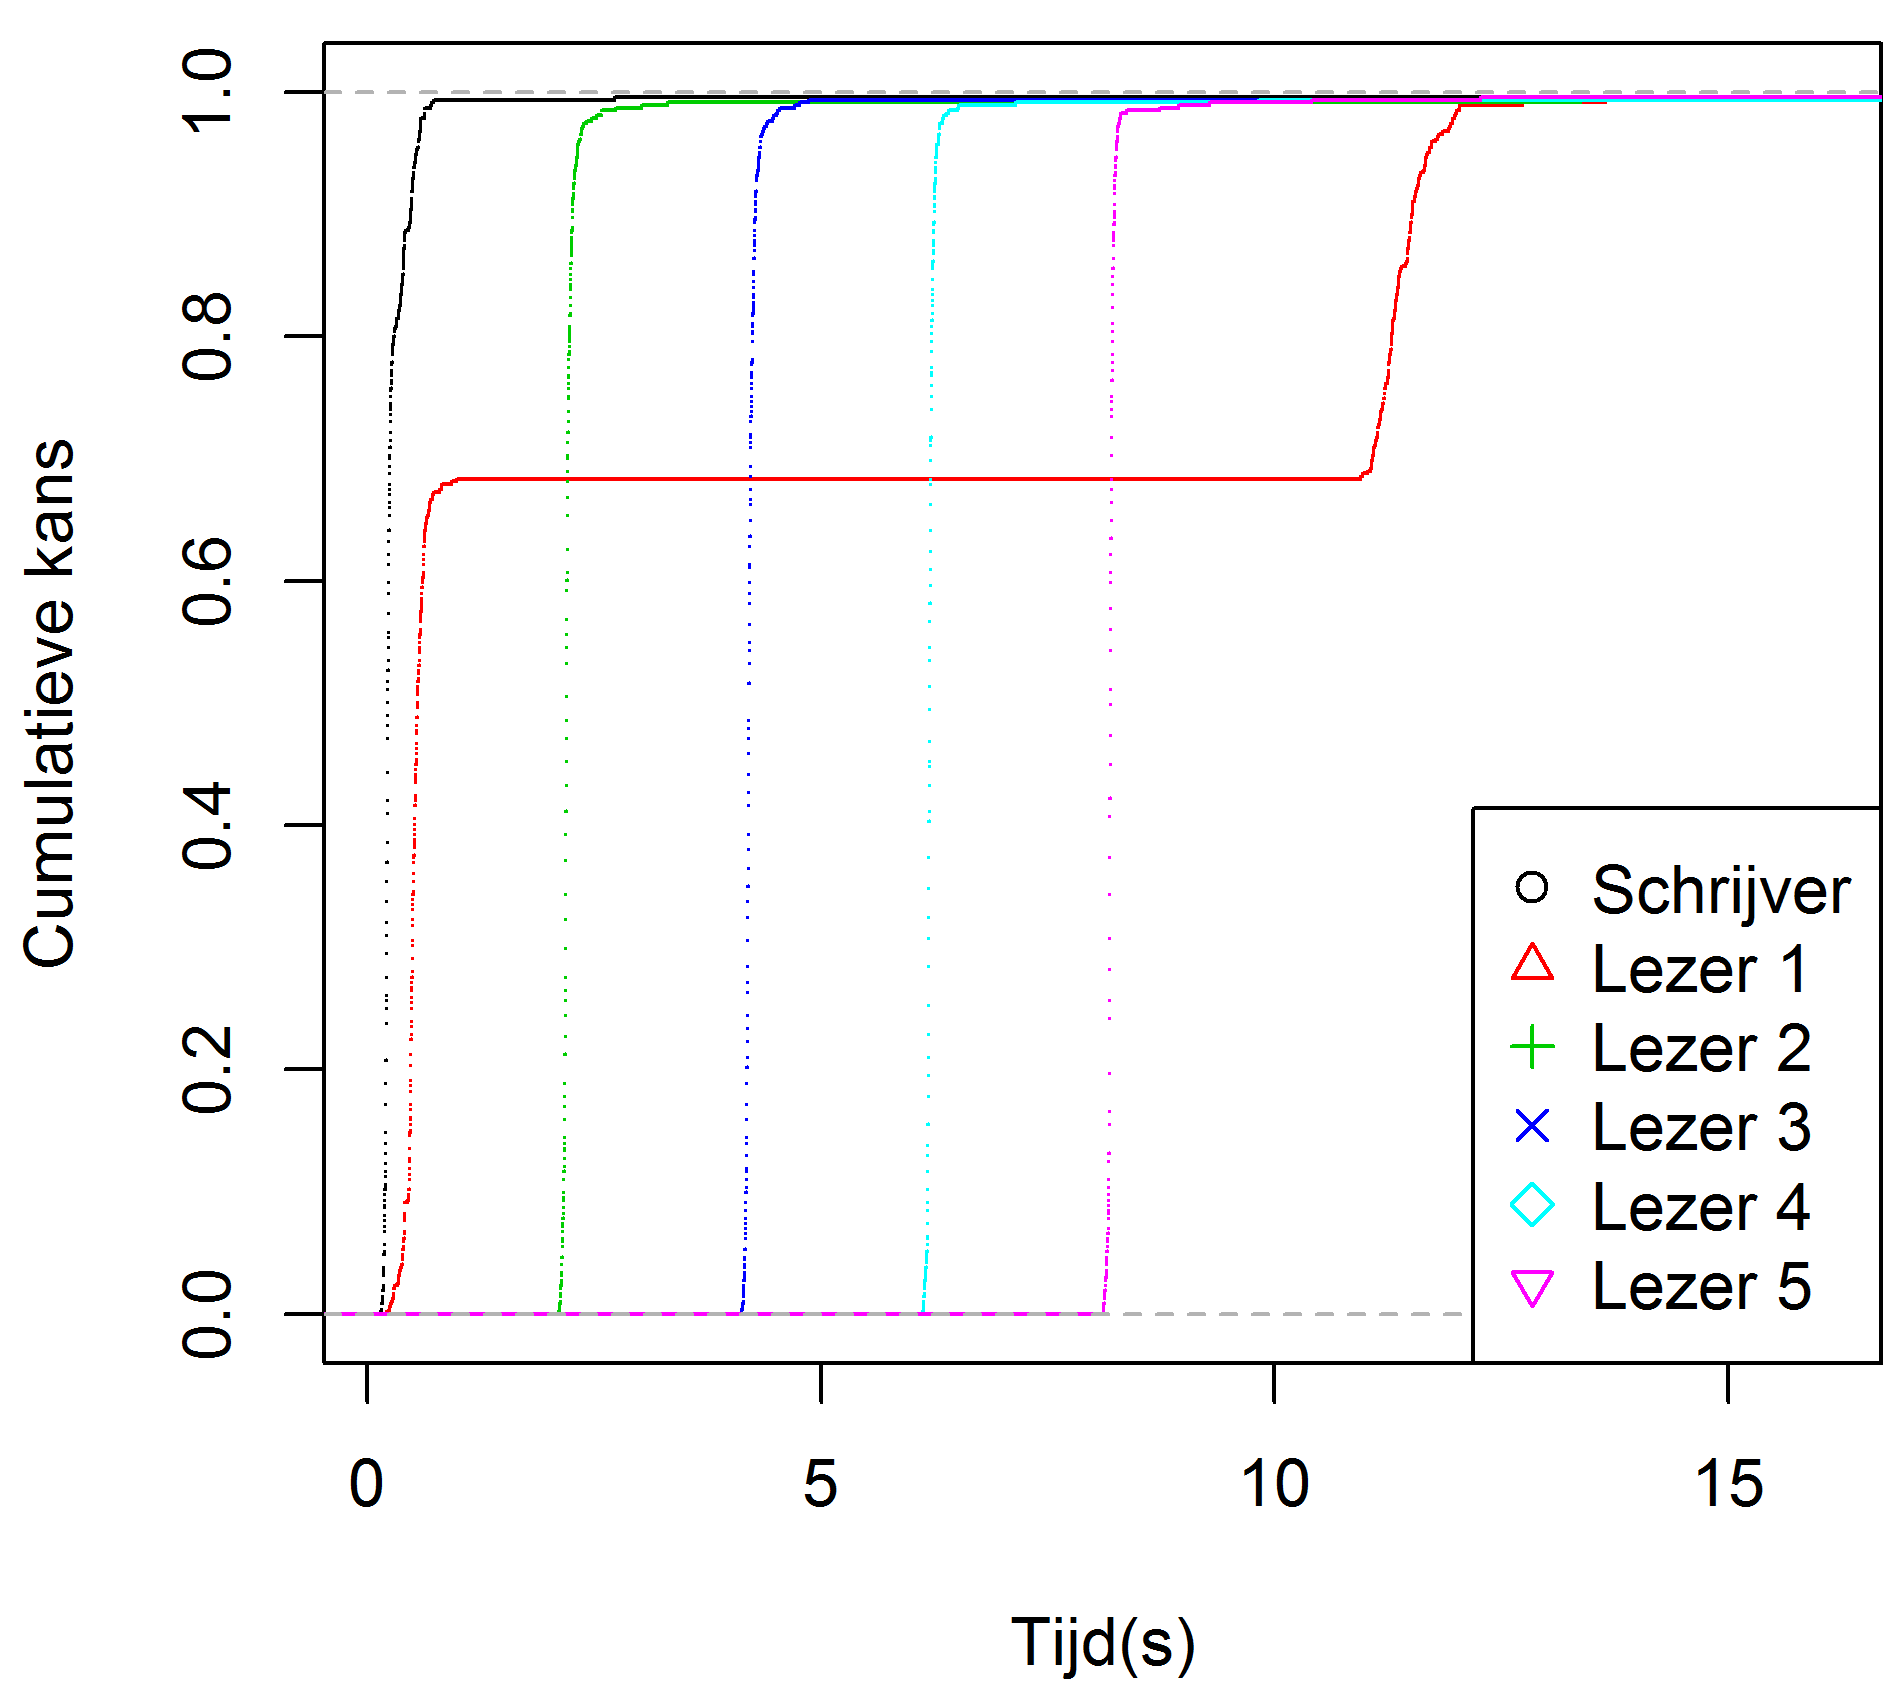
\includegraphics[width=.70\textwidth]{img/Observaties/MongoDB/ECDF-plot-Start-updateRawData-majority-primarypreferred-1}
	\caption{\textbf{Consistentie van MongoDB}: Overzicht van startmoment van consistente leesactie voor het lezen op de primarypreferred }
	\label{fig:consistentie-mongodb-primarypreferred}
\end{figure}
\begin{figure}[htb!] 
	\centering
	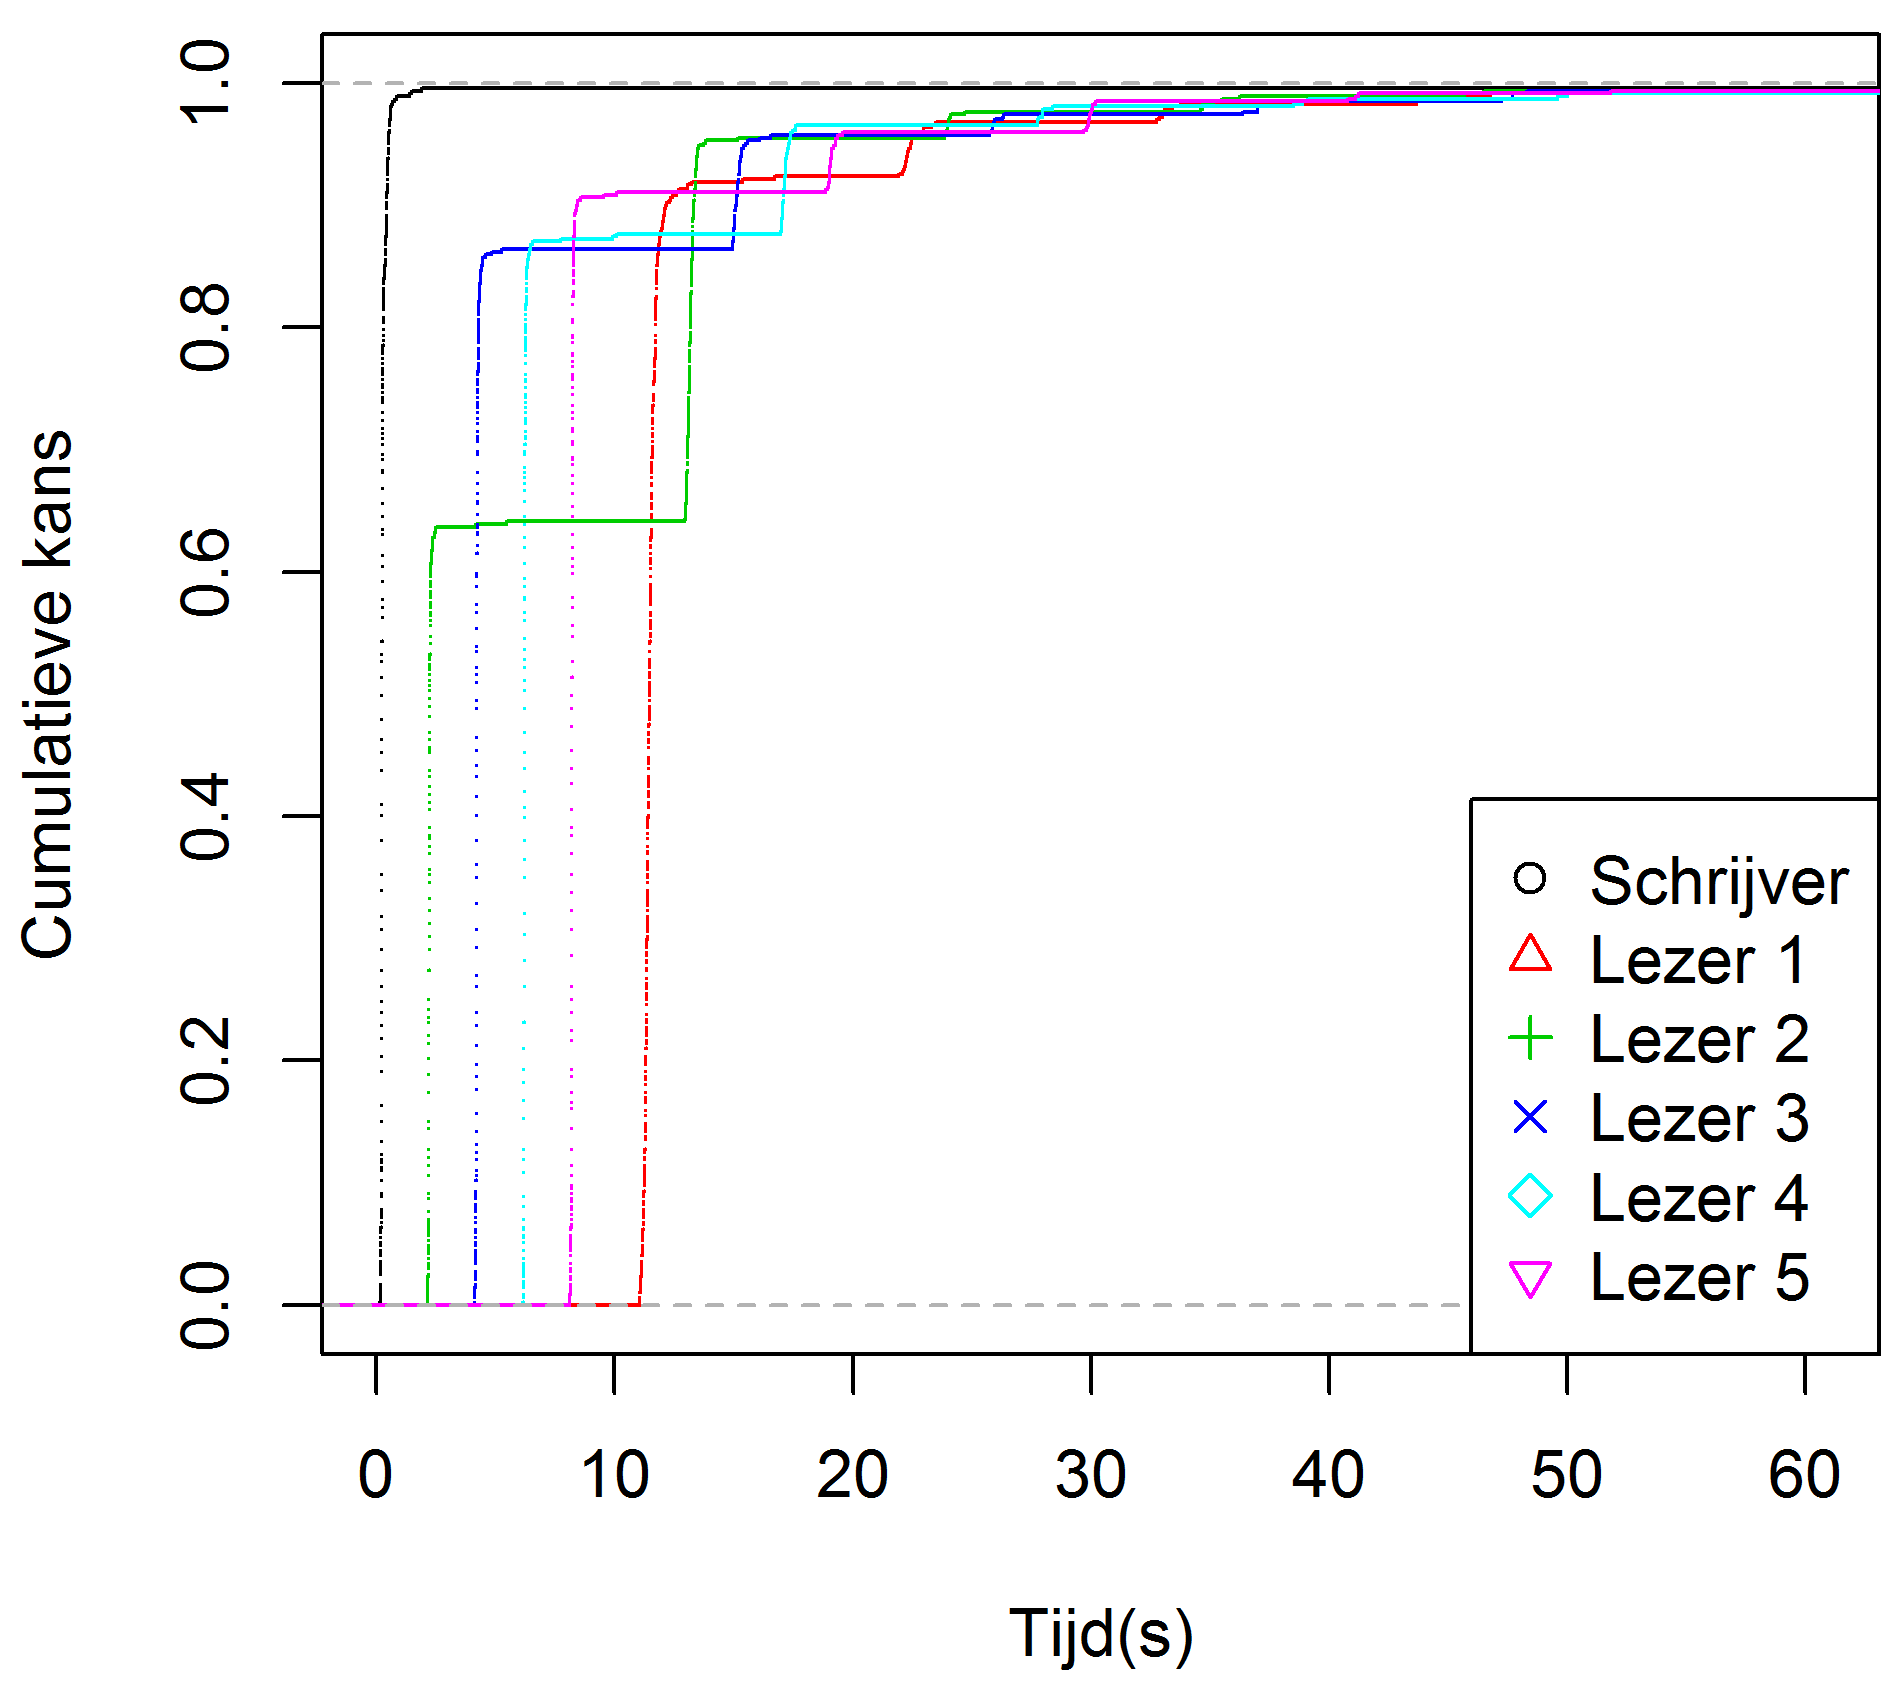
\includegraphics[width=.70\textwidth]{img/Observaties/MongoDB/ECDF-plot-Start-updateRawData-majority-secondary-1}
	\caption{Consistentie van MongoDB: Overzicht van startmoment van consistente leesactie voor het lezen op de secondary }
	\label{fig:consistentie-mongodb-secondary}
\end{figure}
\begin{figure}[htb!] 
	\centering
	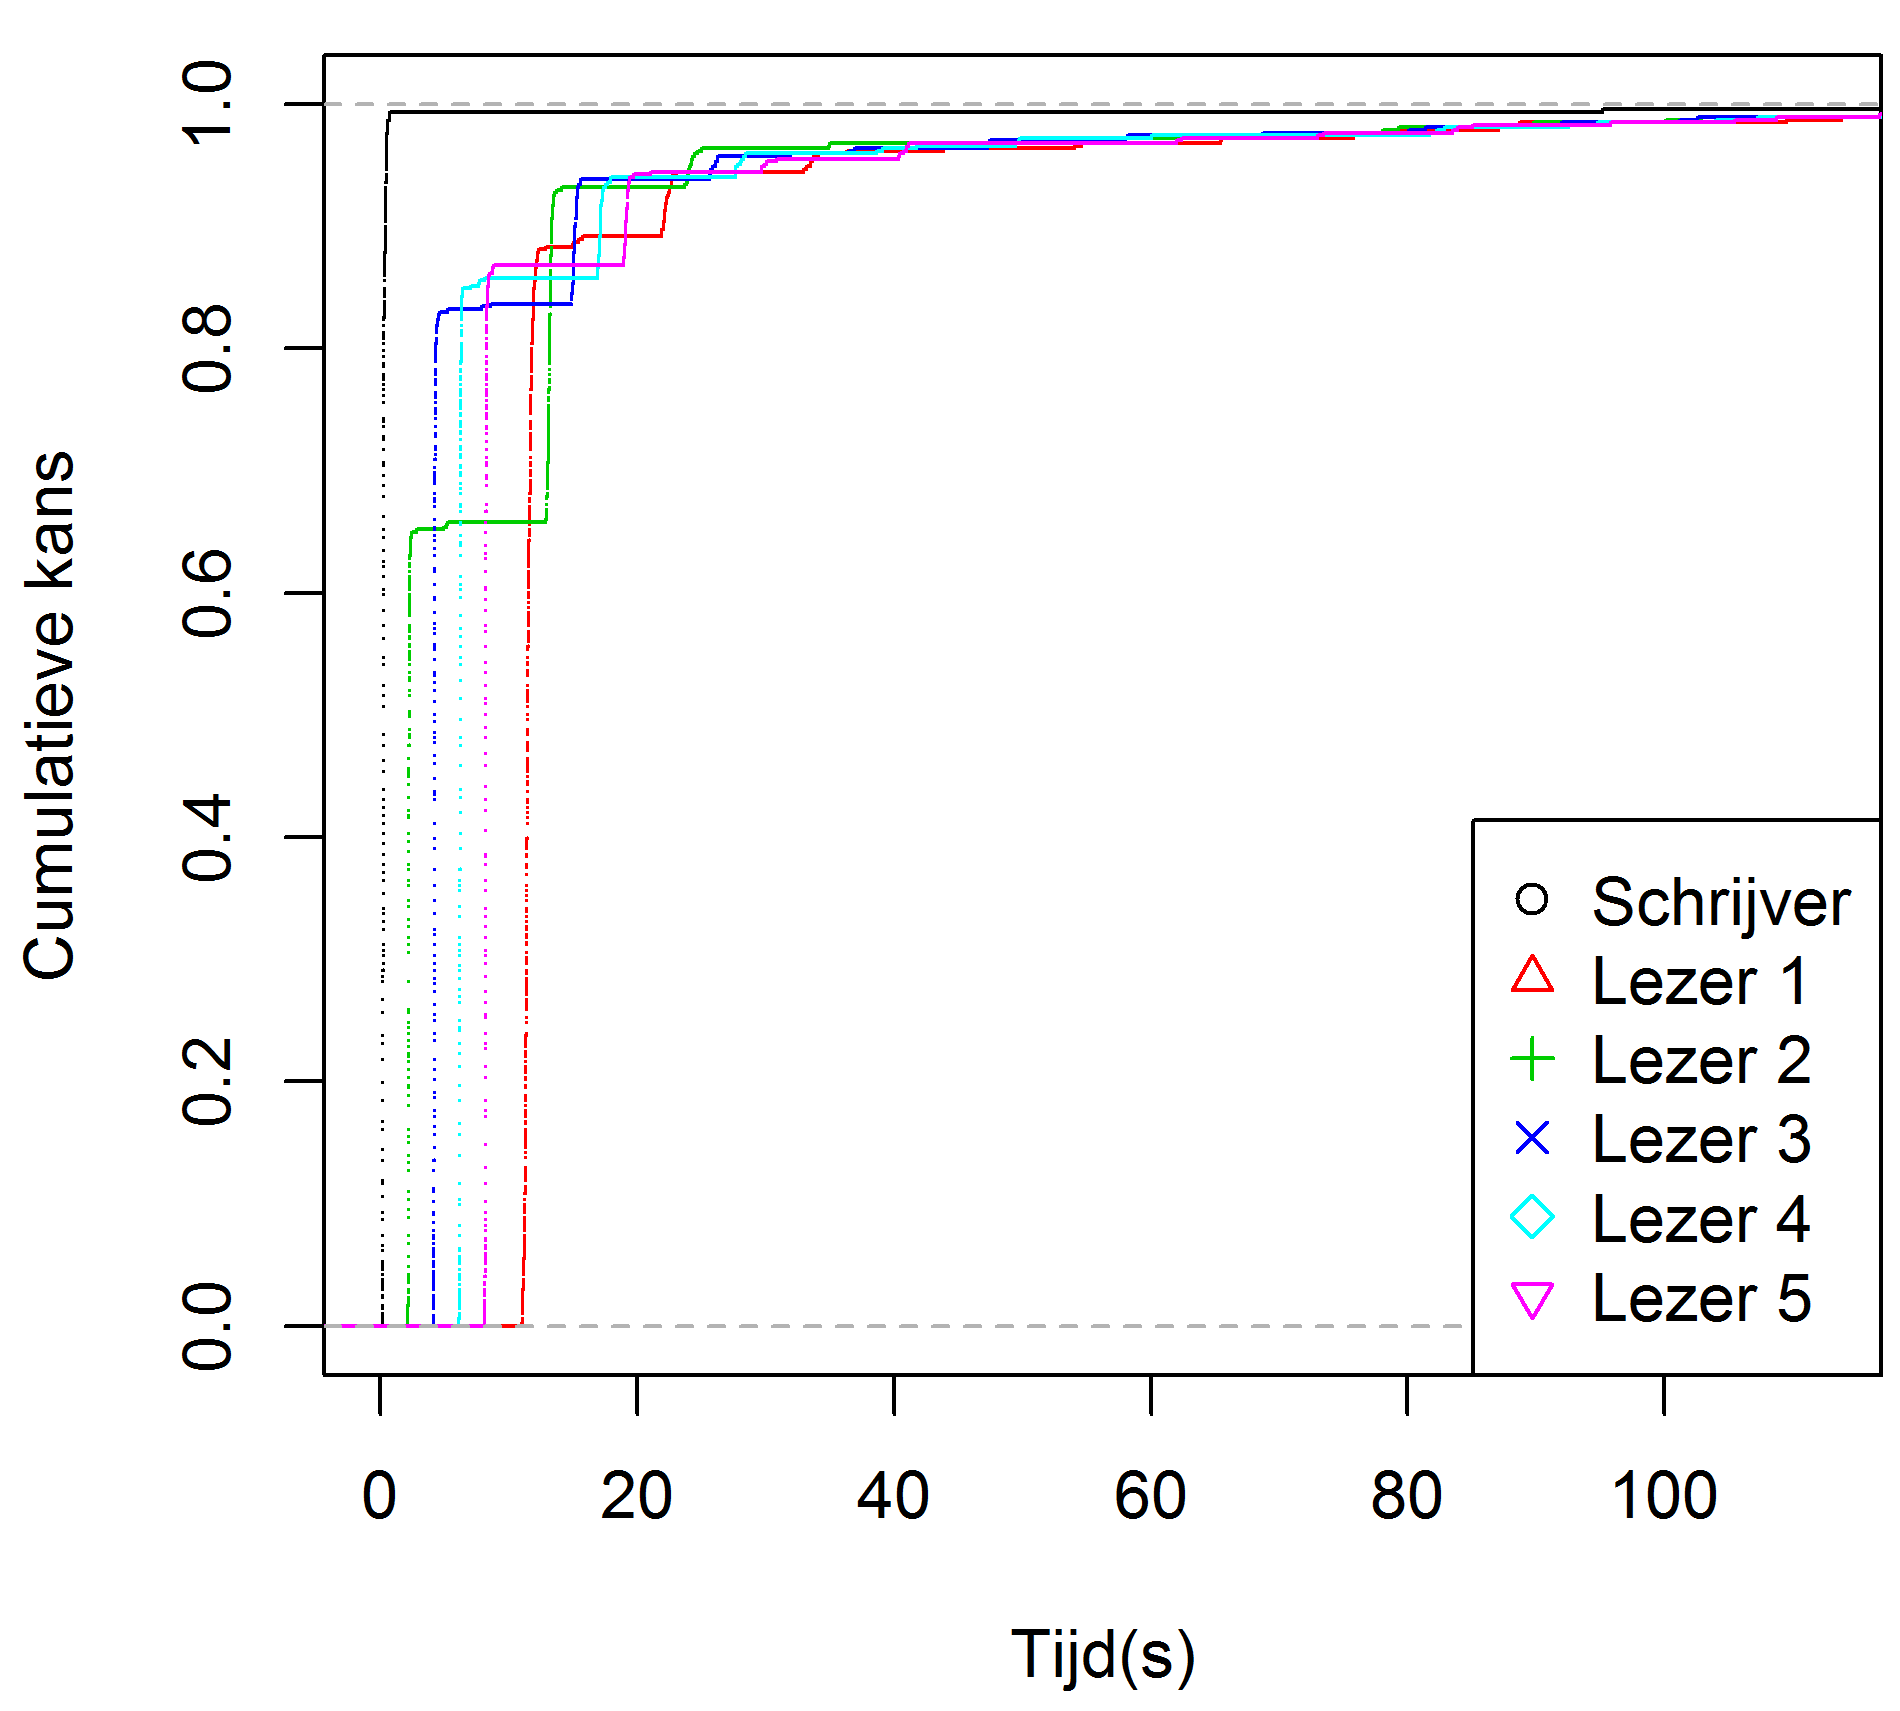
\includegraphics[width=.70\textwidth]{img/Observaties/MongoDB/ECDF-plot-Start-updateRawData-majority-secondarypreferred-1}
	\caption{\textbf{Consistentie van MongoDB}: Overzicht van startmoment van consistente leesactie voor het lezen op de secondarypreferred.  }
	\label{fig:consistentie-mongodb-secondarypreferred}
\end{figure}

\FloatBarrier
\section{Conclusie}
In dit hoofdstuk zijn de resultaten van de verschillende testen getoond voor MongoDB, HBase en Pgpool-II. Het gemeten gedrag is verschillend voor de drie systemen naar beschikbaarheid toe. Ook in consistentie zijn er verschillen tussen HBase en MongoDB. 
In het volgende hoofdstuk zal deze data verder geanalyseerd worden en verklaringen of hypotheses zullen gesteld worden. 